\chapter{RNA-Seq workflow}
\label{chap:transcriptome-workflow}

\todo{Nextflox pipeline; \url{https://www.nature.com/articles/s41598-020-76881-x}, figure 1 notamment pour d'autres exemples de pipeline globales}
% \section{An automated Nextflow pipeline for genome alignement}
%\subsection{Bioinformatic tools for genome alignment}


\section{Objectives} 

\begin{itemize}
\item
  Identification of a \emph{reference signature} matrix, enabling to discriminate specifically any of the cell populations that may contribute to the observed bulk transcriptomic expression.
\item
  Evaluation of the impact of confusing technical and environmental variables on the individual cell transcriptomic expression, such as the effect of the sequencing method, the disease, the gender or the age of the patient.
\end{itemize}


\section{Gene expression databases} 
\label{gene-expression-databases}


\subsection{Import relevant files} 
\label{import-relevant-files}

Most of high-throughput transcriptomic datasets are available on two public repositories: NCBI \emph{Gene Expression Omnibus (GEO)} and ECBI \emph{ArrayExpress.}

GEOs objects are stratified with the following hierarchical structure:

\begin{enumerate}
\item
  A \emph{Platform} object details the general sequencing protocol and lists the probes or gene annotations. Besides, it gathers all the experiences that have been performed under this specific sequencing method. Platform ID follows the following notation: GPL, followed with an accession number.
\item
  A \emph{Series} object identifies a set of Samples associated with the same biological experiment and additionally summarises phenotype features and the global design. It is idnetified with the GSExxx flag.
\item
  A \emph{Sample} record, identified as GSMxxx, describes the conditions under which an individual Sample was handled, the manipulations it undergoes like the platform used, and the abundance measurement of each annotated transcript.
\end{enumerate}

The second biggest source of public datasets is \emph{ArrayExpress}, with differs from GEO with additional restrictions on the format of the datasets submitted, imposing to make them MIAME-compliant. Currently, 76,635 studies are represented in the ArrayExpress compendium. The general format is for each repository, a zipped MAGE-TAB document which splits itself into an \emph{Investigation Description Format (IDF)} file, equivalent to the MIAME experimental data of the eset object and describing top-level protocol experiences: \href{https://rdrr.io/pkg/Biobase/man/abstract.html}{\texttt{Biobase::experimentData}}, \emph{Array Design Format (ADF)}, equivalent to the feature data: \href{https://rdrr.io/pkg/Biobase/man/featureData.html}{\texttt{Biobase::fData}}, with the position (for microarray only) and the annotation of the measured transcripts, \emph{Sample and Data Relationship Format (SDRF)}, equivalent to the phenotype data: \href{https://rdrr.io/pkg/Biobase/man/phenoData.html}{\texttt{Biobase::pData}} and eventually the raw and processed data files, that store transcriptomic expression.

While the packages \href{http://seandavi.github.io/GEOquery/articles/GEOquery.html}{\texttt{GEOquery}}, \autocite{R-GEOquery}, \autocite{GEOquery2007}, and \href{https://bioconductor.org/packages/release/bioc/vignettes/ArrayExpress/inst/doc/ArrayExpress.pdf}{\texttt{ArrayExpress}}, \autocite{R-ArrayExpress}, \autocite{ArrayExpress2009}, have been designed to automatically query and fetch online databases, they are rather restricted to a specific format, unfortunately rarely met in practice. Depending on the level of precision required, along with general feature description files, we let the user to choose between raw or pre-processed data (generally, a tab-delimited file enumerating for each probe or identified transcript its total expression). In practice, one of the major bottlenecks is the absence of pre-processed expression data in the majority of RNASeq experiments, and the lack of standardisation of raw datasets. We have therefore attempted to partially resolve these limitations by respectively developing proprietary functions \texttt{bbcFetching::import\_normalised\_data} and \texttt{bbcFetching:::import\_raw\_files} for normalised and raw datasets, both functions attempting at first to parse local files, then fetch them online, and finally homogenises the output into an ExpressionSet object:

In addition, we display respectively the architecture of ArrayExpress, GEO and SRA databases\footnote{This last repository is specifically dedicated to store high throughput sequencing experiments, and reveals its full potential as un unlimited and parallel data storage, at the raw read alignment level, along with NCBI GEO and EBI ArrayExpress databases. Currently, the R package \href{http://www.ncbi.nlm.nih.gov/books/NBK47537/}{SRAdb}, \autocite{R-SRAdb}, \autocite{SRAdb2013}, is recommended for automatically querying, downloading and extracting alignment information}, in Fig.\Cref{fig:databases-schema-pdf}.

\begin{figure}

{\centering \subfloat[Relation database and user API interface, from  \href{https://ecoliwiki.org/colipedia/index.php/Gene_Expression_Omnibus_(GEO)}{Wiki GEO} 
\label{fig:databases-schema-pdf-1}]{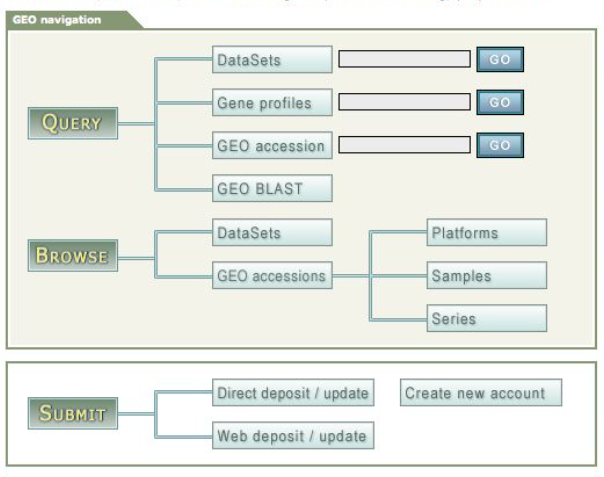
\includegraphics[width=0.45\linewidth]{figures/ERD_GEO} }\subfloat[The \href{https://www.bioconductor.org/packages/release/bioc/vignettes/SRAdb/inst/doc/SRAdb.pdf}{ArrayExpress} architecture, with user functionality detailled at the bottom on its vignette.\label{fig:databases-schema-pdf-2}]{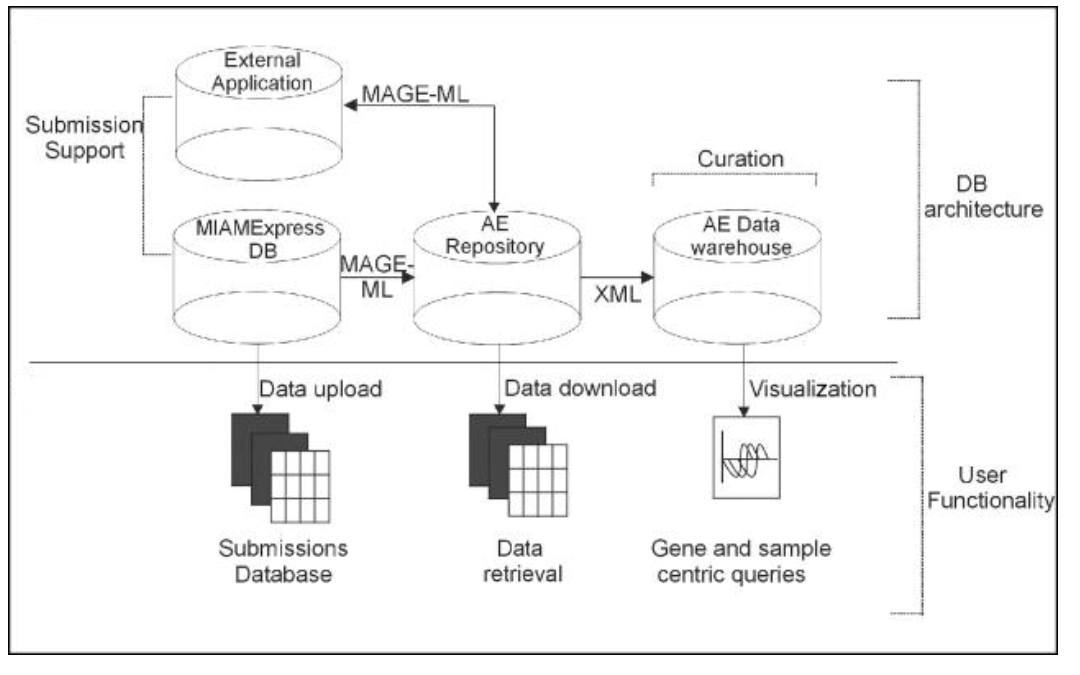
\includegraphics[width=0.45\linewidth]{figures/ERD_ArrayExpress} }\newline\subfloat[The graphical representation describing the entity relationships between the tables in \href{https://www.bioconductor.org/packages/release/bioc/vignettes/SRAdb/inst/doc/SRAdb.pdf}{SRAdb vignette}\label{fig:databases-schema-pdf-3}]{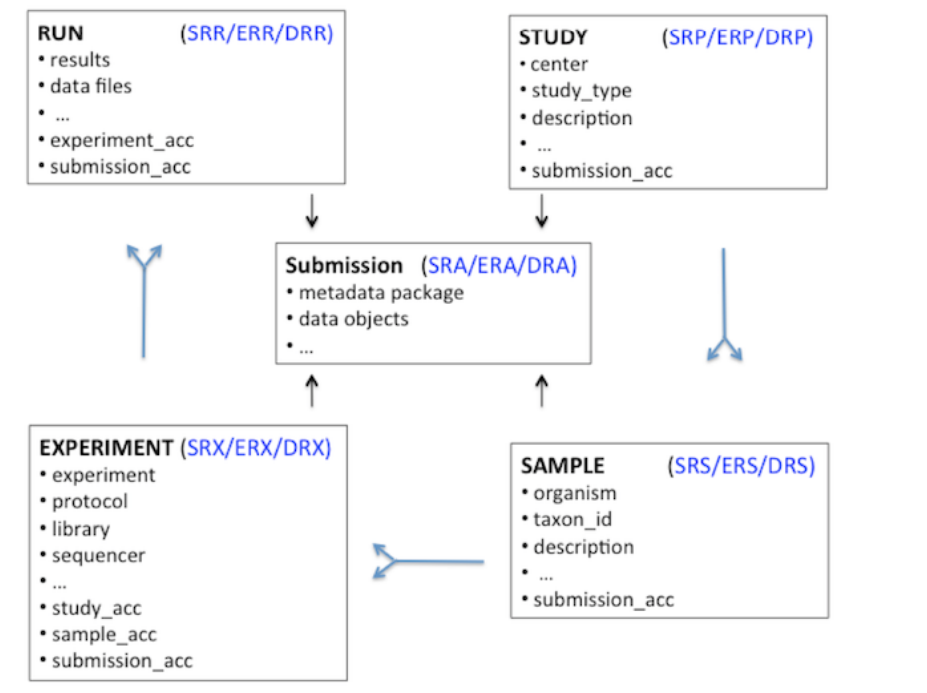
\includegraphics[width=0.45\linewidth]{figures/ERD_SRAdb} }

}

\caption{We display respectively the ERD (\emph{Entity-Relationship Diagram}), of GEO, ArrayExpress and SRA databases}\label{fig:databases-schema-pdf}
\end{figure}


\subsection{Data wrangling with ExpressionSet}\label{data-wrangling-with-expressionset}

An ExpressionSet object is composed of an expression matrix, a gene annotation dataset
and a phenotype dataset storing patient information, associated with general metadata stored in a MIAME object. In this section, we enumerate all the data formatting and quality check-ups performed to clean and leverage essential information from ExpressionSet:

\begin{enumerate}
\def\labelenumi{\arabic{enumi}.}
\item
  Data format: We require that transcriptomic expression is stored in a matrix, and that the annotation sets are \texttt{data.frame} objects.
\item
  All elements composing the eset must be documented with colnames and rownames, such that the colnames of the eset match the rownames of the \texttt{pData} object (correspond to unique identification of samples) and its rownames match the rownames of the \texttt{fData} object (unique identification of transcripts). We recall the general structure of ExpressionSet objects as well as the operations required to manipulate them in in Fig.\Cref{fig:databases-schema-pdf}.
\item
  Variable types: carefully prepare samples and features annotation data by formatting numerical variables in numeric format and converting textual variables as factors. When comparing several eset objects, it is relevant to keep track of factor assignment, and homogenises them across batches. About missing values, we marked unequivocally using the \emph{reserved variable name} \texttt{NA}, see sub\Cref{subsubsec:sample-annotation} for details.
\item
  Gene annotation: this step ensures that gene ID used can be uniquely mapped to their corresponding most updated HGNC symbol. We can additionally filter out genes that are not involved in any of the biological functions of interest, see details in sub\Cref{subsubsec:gene-annotation}.
\item
  (Optional) There is currently a strong lack of standard nomenclature to refer to cell types. We thus provide in sub\Cref{subsubsec:cell-type-annotation} helper functions to homogenise them across samples. Similarly, we may as well use ontologies to uniquely identify diseases or tissues.
\end{enumerate}





\begin{figure}

{\centering \subfloat[Structure of a \href{https://www.researchgate.net/figure/Structure-of-Bioconductors-ExpressionSet-class_fig1_326163413}{Bioconductor's ExpressionSet} object \autocite{Biobase2015}--\autocite{klaus_reisenauer18}.\label{fig:expressionset-structure-pdf-1}]{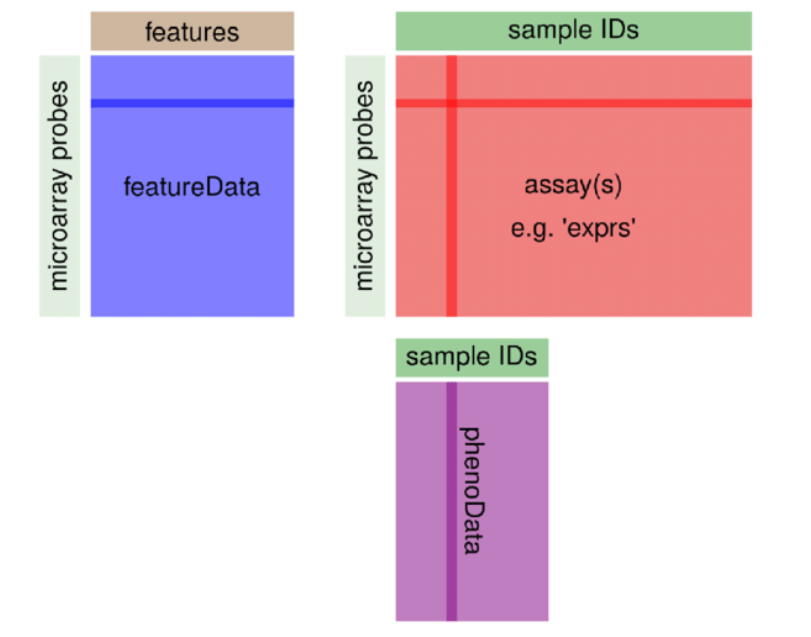
\includegraphics[width=0.45\linewidth]{figures/expressionset_structure} }\subfloat[The \href{https://combine-australia.github.io/2017-05-19-bioconductor-melbourne/data_structures.html}{SummarizedExperiment} object \autocite{R-SummarizedExperiment} is a generalisation of ExpressionSet. It is traditionally used to store the results of several experiences (provided at least some Gene IDs match). Besides, this format is required in some normalisation and differential analysis functions, notably for the \emph{vst} normalisation applied by \href{https://bioconductor.org/packages/release/bioc/vignettes/DESeq2/inst/doc/DESeq2.html}{DeSeq2} Bioconductor package \autocite{R-DESeq2}, \autocite{DESeq22014}.\label{fig:expressionset-structure-pdf-2}]{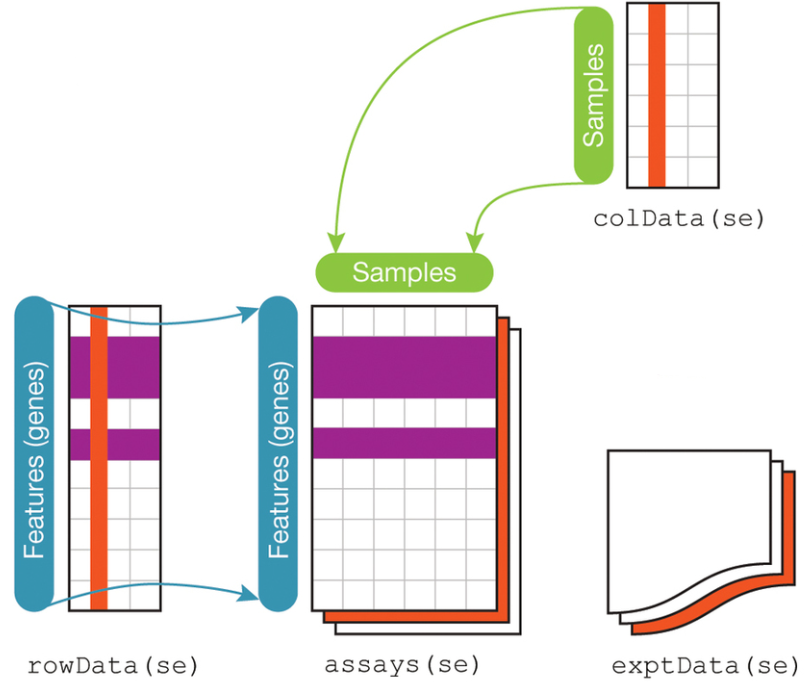
\includegraphics[width=0.45\linewidth]{figures/summarised_experiment_structure} }

}

\caption{General structure of the objects most commonly used in R to store transcriptomic data}\label{fig:expressionset-structure-pdf}
\end{figure}


\subsubsection{Sample annotation} 
\label{subsubsec:sample-annotation}

Part of this tedious data cleaning is automatically carried out with function \href{https://rdrr.io/pkg/bbcWrangling/man/clean_eset_names.html}{\texttt{bbcWrangling::clean\_eset\_names()}}, which proceeds in three steps:

\begin{enumerate}
\def\labelenumi{\arabic{enumi}.}
\item
  First, simplify the identification colnames of objects \href{https://rdrr.io/pkg/Biobase/man/phenoData.html}{\texttt{Biobase::pData}} and \href{https://rdrr.io/pkg/Biobase/man/featureData.html}{\texttt{Biobase::fData}}, mostly by complying them with the ruling names' syntax of R.
\item
  All non-ascii characters can be trimmed, however, perform this operation with care, since some of the characters of gene names may not comply with ASCII character encoding format.
\item
  The most useful function, removes any constant colname of object \texttt{Biobase::pData()}, and stores it as a \texttt{MIAME} object in slot \texttt{Biobase::experimentData}. We mean by \emph{constant} any column that stores information common to all the samples, or patients, considered for the experiment, which can be typically the sequencing technology, the general experimental name or setting, or general information about laboratory and biologists contacts.
\end{enumerate}

In addition to simplify the manual curation of phenotype data, these general management operations help identifying variables of interest, as well as confusing variables (for instance, batch replicates), and reduces the storage space taken by the eset object. For instance, the size taken by the phenotype dataset in memory hardware shifts from 322.8 Kb and 64, to 228 Kb and 26 on the cleaned eset.

However, while part of the automated data curation is performed by \href{https://rdrr.io/pkg/bbcWrangling/man/clean_eset_names.html}{\texttt{bbcWrangling::clean\_eset\_names()}}, there is still a need of manual curation, and we displayed below some common data wrangling operations to be performed on purified cell expression sets, respectively for GEO ID 149050 and 137143:

\begin{itemize}
\item
  Rename columns, such that shared phenotype information, are labelled consistently across several Expression Sets, for instance the columns returning the cell assignement or the patient id
\item
  Convert to factor any categorical variable which may contribute to biological or technical variability, since they will be required for batch correction and downstream analysis. Perform similarly for continuous values. For the last two experiences described, we identified three shared categorical variables of interest: patient assignment, cell type assignment and disease phenotype, and one continuous variable, age of the patient.
\item
  About categorical variables, you may attempt to merge closely related cell factors to gain statistical power and promote comparison across samples, a point further developed in sub\Cref{subsubsec:cell-type-annotation}
\end{itemize}

\begin{Shaded}
\begin{Highlighting}[]
\NormalTok{gse149050\_pheno\_data }\OtherTok{\textless{}{-}}\NormalTok{ Biobase}\SpecialCharTok{::}\FunctionTok{pData}\NormalTok{(gse149050\_raw\_count\_clean) }
\NormalTok{gse149050\_pheno\_data }\OtherTok{\textless{}{-}}\NormalTok{ gse149050\_pheno\_data  }\SpecialCharTok{\%\textgreater{}\%}
\NormalTok{  dplyr}\SpecialCharTok{::}\FunctionTok{select}\NormalTok{(}\FunctionTok{c}\NormalTok{(}\StringTok{"geo\_accession"}\NormalTok{,}
                  \StringTok{"age\_ch1"}\NormalTok{, }\StringTok{"cell\_type\_ch1"}\NormalTok{,}
                  \StringTok{"patientuid\_ch1"}\NormalTok{, }\StringTok{"relation\_1"}\NormalTok{,}
                  \StringTok{"disease\_state\_ch1"}\NormalTok{)) }\SpecialCharTok{\%\textgreater{}\%}
\NormalTok{  dplyr}\SpecialCharTok{::}\FunctionTok{rename}\NormalTok{(}\AttributeTok{sample\_id=}\StringTok{"geo\_accession"}\NormalTok{, }\AttributeTok{disease=}\StringTok{"disease\_state\_ch1"}\NormalTok{) }\SpecialCharTok{\%\textgreater{}\%}
\NormalTok{  dplyr}\SpecialCharTok{::}\FunctionTok{rename\_with}\NormalTok{(}\SpecialCharTok{\textasciitilde{}}\FunctionTok{gsub}\NormalTok{(}\StringTok{"\_(ch)*1$"}\NormalTok{, }\StringTok{""}\NormalTok{, .x)) }\SpecialCharTok{\%\textgreater{}\%}
\NormalTok{  dplyr}\SpecialCharTok{::}\FunctionTok{mutate}\NormalTok{(}\AttributeTok{patient\_id=}\NormalTok{stringr}\SpecialCharTok{::}\FunctionTok{str\_extract}\NormalTok{(patientuid,}
                                                \AttributeTok{pattern =} \StringTok{"\^{}[[:upper:]]\{1\}[[:digit:]]+"}\NormalTok{),}
                \AttributeTok{disease=}\NormalTok{forcats}\SpecialCharTok{::}\FunctionTok{fct\_collapse}\NormalTok{(}\FunctionTok{as.factor}\NormalTok{(disease),}
                                              \AttributeTok{hc=}\FunctionTok{c}\NormalTok{(}\StringTok{"healthy control"}\NormalTok{),}
                                              \StringTok{"sle"}\OtherTok{=}\FunctionTok{c}\NormalTok{(}\StringTok{"systemic lupus erythematosus (SLE)"}\NormalTok{)),}
                \AttributeTok{age=}\FunctionTok{as.numeric}\NormalTok{(age), }
                \AttributeTok{URL=}\NormalTok{stringr}\SpecialCharTok{::}\FunctionTok{str\_extract}\NormalTok{(relation, }\AttributeTok{pattern =} \StringTok{"(?\textless{}=SRA: )(.*?)$"}\NormalTok{),}
                \AttributeTok{platform=}\StringTok{"GPL16791"}\NormalTok{, }\AttributeTok{tissue=}\StringTok{"blood"}\NormalTok{,}
                \FunctionTok{across}\NormalTok{(}\FunctionTok{c}\NormalTok{(}\StringTok{"cell\_type"}\NormalTok{, }\StringTok{"disease"}\NormalTok{, }\StringTok{"patient\_id"}\NormalTok{),}
                       \SpecialCharTok{\textasciitilde{}}\NormalTok{ janitor}\SpecialCharTok{::}\FunctionTok{make\_clean\_names}\NormalTok{(.x, }\AttributeTok{allow\_dupes =} \ConstantTok{TRUE}\NormalTok{) }\SpecialCharTok{\%\textgreater{}\%}
\NormalTok{                         forcats}\SpecialCharTok{::}\FunctionTok{as\_factor}\NormalTok{())) }\SpecialCharTok{\%\textgreater{}\%}
  \FunctionTok{select}\NormalTok{(}\SpecialCharTok{{-}}\FunctionTok{c}\NormalTok{(patientuid, relation, URL))}
\NormalTok{gse149050\_raw\_count\_clean }\OtherTok{\textless{}{-}}\NormalTok{ bbcWrangling}\SpecialCharTok{::}\FunctionTok{update\_eset\_object}\NormalTok{(gse149050\_raw\_count\_clean,}
                                                              \AttributeTok{phenotype\_data =}\NormalTok{ gse149050\_pheno\_data)}
\end{Highlighting}
\end{Shaded}

\begin{Shaded}
\begin{Highlighting}[]
\NormalTok{pheno\_data\_137143 }\OtherTok{\textless{}{-}}\NormalTok{ Biobase}\SpecialCharTok{::}\FunctionTok{pData}\NormalTok{(gse137143\_TPM\_count\_clean)}
\NormalTok{pheno\_data\_137143 }\OtherTok{\textless{}{-}}\NormalTok{ pheno\_data\_137143  }\SpecialCharTok{\%\textgreater{}\%}
\NormalTok{  dplyr}\SpecialCharTok{::}\FunctionTok{select}\NormalTok{(}\SpecialCharTok{{-}}\FunctionTok{c}\NormalTok{(}\StringTok{"title"}\NormalTok{, }\StringTok{"srx\_id"}\NormalTok{)) }\SpecialCharTok{\%\textgreater{}\%}
\NormalTok{  dplyr}\SpecialCharTok{::}\FunctionTok{mutate}\NormalTok{(}\AttributeTok{age=}\FunctionTok{as.numeric}\NormalTok{(age),  }\AttributeTok{tissue=}\StringTok{"blood"}\NormalTok{, }\AttributeTok{platform=}\StringTok{"GPL24676"}\NormalTok{,}
                \AttributeTok{disease =}\NormalTok{ forcats}\SpecialCharTok{::}\FunctionTok{fct\_collapse}\NormalTok{(}\FunctionTok{as.factor}\NormalTok{(disease),}
                                                \AttributeTok{hc=}\FunctionTok{c}\NormalTok{(}\StringTok{"NA"}\NormalTok{),}
                                                \AttributeTok{ms=}\FunctionTok{c}\NormalTok{(}\StringTok{"CIS"}\NormalTok{, }\StringTok{"PP"}\NormalTok{, }\StringTok{"RIS"}\NormalTok{, }\StringTok{"RR"}\NormalTok{, }\StringTok{"SP"}\NormalTok{, }\StringTok{"Unknown"}\NormalTok{)),}
                \FunctionTok{across}\NormalTok{(}\FunctionTok{c}\NormalTok{(}\StringTok{"cell\_type"}\NormalTok{, }\StringTok{"disease"}\NormalTok{, }\StringTok{"patient\_id"}\NormalTok{),}
                       \SpecialCharTok{\textasciitilde{}}\NormalTok{ janitor}\SpecialCharTok{::}\FunctionTok{make\_clean\_names}\NormalTok{(.x, }\AttributeTok{allow\_dupes =} \ConstantTok{TRUE}\NormalTok{) }\SpecialCharTok{\%\textgreater{}\%}
\NormalTok{                         forcats}\SpecialCharTok{::}\FunctionTok{as\_factor}\NormalTok{()),}
                \AttributeTok{cell\_type =}\NormalTok{ forcats}\SpecialCharTok{::}\FunctionTok{fct\_collapse}\NormalTok{(cell\_type,}
                                                  \AttributeTok{c\_mo =} \StringTok{"cd14\_monocytes"}\NormalTok{,}
                                                  \AttributeTok{t\_cells=}\FunctionTok{c}\NormalTok{(}\StringTok{"cd4\_t\_cells"}\NormalTok{, }\StringTok{"cd8\_t\_cells"}\NormalTok{))) }\SpecialCharTok{\%\textgreater{}\%}
\NormalTok{                tidyr}\SpecialCharTok{::}\FunctionTok{unite}\NormalTok{(}\AttributeTok{col=}\StringTok{"sample\_id"}\NormalTok{, patient\_id, cell\_type, }\AttributeTok{sep =} \StringTok{"\_"}\NormalTok{, }\AttributeTok{remove =} \ConstantTok{FALSE}\NormalTok{) }
\NormalTok{gse137143\_TPM\_count\_clean }\OtherTok{\textless{}{-}}\NormalTok{ bbcWrangling}\SpecialCharTok{::}\FunctionTok{update\_eset\_object}\NormalTok{(gse137143\_TPM\_count\_clean,}
                                                              \AttributeTok{phenotype\_data =}\NormalTok{ pheno\_data\_137143)}
\end{Highlighting}
\end{Shaded}

In our example, we decided to concatenate closely related cell populations, by summing up their expressions within the same individual, based on our linear assumption of the reconstruction of the whole mixture:

\begin{Shaded}
\begin{Highlighting}[]
\CommentTok{\# helper function to aggregate expression and phenotype feature, using a common factor}
\NormalTok{gse137143\_TPM\_count\_clean }\OtherTok{\textless{}{-}}\NormalTok{ bbcWrangling}\SpecialCharTok{::}\FunctionTok{aggregate\_by\_pdata}\NormalTok{(gse137143\_TPM\_count\_clean,}
                                                                  \AttributeTok{col=}\FunctionTok{c}\NormalTok{(}\StringTok{"sample\_id"}\NormalTok{), sum)}
\end{Highlighting}
\end{Shaded}

We display respectively in Tables \Cref{tab:phenotype-description-pdf} and \Cref{tab:phenotype-description-second-pdf}, using function \texttt{bbcViz::display\_table()}, some of the phenotype variables of interest, as well as potential confusing ones. All these variables may contribute to the global transcriptomic variability across samples:

\global\setlength{\Oldarrayrulewidth}{\arrayrulewidth}

\global\setlength{\Oldtabcolsep}{\tabcolsep}

\setlength{\tabcolsep}{0pt}

\renewcommand*{\arraystretch}{1.5}



\providecommand{\ascline}[3]{\noalign{\global\arrayrulewidth #1}\arrayrulecolor[HTML]{#2}\cline{#3}}

\begin{longtable}[c]{|p{1.31in}|p{1.04in}|p{0.93in}|p{1.20in}}

\caption{Visualise\ some\ phenotype\ characteristics\ of\ the\ patients\ from\ cohort\ GEO\ 149050}
\label{tab:phenotype-description-pdf}\\

\hhline{>{\arrayrulecolor[HTML]{000000}\global\arrayrulewidth=0pt}->{\arrayrulecolor[HTML]{000000}\global\arrayrulewidth=0pt}->{\arrayrulecolor[HTML]{000000}\global\arrayrulewidth=0pt}->{\arrayrulecolor[HTML]{000000}\global\arrayrulewidth=0pt}-}

\multicolumn{1}{>{\cellcolor[HTML]{95D1DC}\raggedright}m{\dimexpr 1.31in+0\tabcolsep}}{\textcolor[HTML]{000000}{\fontsize{12}{12}\selectfont{\textbf{sample\_id}}}} & \multicolumn{1}{>{\cellcolor[HTML]{95D1DC}\raggedright}m{\dimexpr 1.04in+0\tabcolsep}}{\textcolor[HTML]{000000}{\fontsize{12}{12}\selectfont{\textbf{cell\_type}}}} & \multicolumn{1}{>{\cellcolor[HTML]{95D1DC}\raggedright}m{\dimexpr 0.93in+0\tabcolsep}}{\textcolor[HTML]{000000}{\fontsize{12}{12}\selectfont{\textbf{disease}}}} & \multicolumn{1}{>{\cellcolor[HTML]{95D1DC}\raggedleft}m{\dimexpr 1.2in+0\tabcolsep}}{\textcolor[HTML]{000000}{\fontsize{12}{12}\selectfont{\textbf{age}}}} \\

\noalign{\global\arrayrulewidth 0pt}\arrayrulecolor[HTML]{000000}

\hhline{>{\arrayrulecolor[HTML]{FFFFFF}\global\arrayrulewidth=0.75pt}->{\arrayrulecolor[HTML]{FFFFFF}\global\arrayrulewidth=0.75pt}->{\arrayrulecolor[HTML]{FFFFFF}\global\arrayrulewidth=0.75pt}->{\arrayrulecolor[HTML]{FFFFFF}\global\arrayrulewidth=0.75pt}-}\endhead



\multicolumn{4}{>{\raggedright}m{\dimexpr 4.49in+6\tabcolsep}}{\textcolor[HTML]{000000}{\fontsize{11}{11}\selectfont{(10\ first\ lines\ /\ \ 288\ lines)}}} \\

\noalign{\global\arrayrulewidth 0pt}\arrayrulecolor[HTML]{FFFFFF}

\endfoot



\multicolumn{1}{>{\cellcolor[HTML]{FFFFFF}\raggedright}m{\dimexpr 1.31in+0\tabcolsep}}{\textcolor[HTML]{000000}{\fontsize{12}{12}\selectfont{GSM4489145}}} & \multicolumn{1}{>{\cellcolor[HTML]{FFFFFF}\raggedright}m{\dimexpr 1.04in+0\tabcolsep}}{\textcolor[HTML]{000000}{\fontsize{12}{12}\selectfont{t\_cells}}} & \multicolumn{1}{>{\cellcolor[HTML]{FFFFFF}\raggedright}m{\dimexpr 0.93in+0\tabcolsep}}{\textcolor[HTML]{000000}{\fontsize{12}{12}\selectfont{hc}}} & \multicolumn{1}{>{\cellcolor[HTML]{FFFFFF}\raggedleft}m{\dimexpr 1.2in+0\tabcolsep}}{\textcolor[HTML]{000000}{\fontsize{12}{12}\selectfont{33.0}}\textcolor[HTML]{000000}{\fontsize{12}{12}\selectfont{\ \ }}
\includegraphics[width=0.5in, height=0.2in]{figure-latex/phenotype-description-pdf-3.png}} \\

\noalign{\global\arrayrulewidth 0pt}\arrayrulecolor[HTML]{000000}





\multicolumn{1}{>{\raggedright}m{\dimexpr 1.31in+0\tabcolsep}}{\textcolor[HTML]{000000}{\fontsize{12}{12}\selectfont{GSM4489146}}} & \multicolumn{1}{>{\raggedright}m{\dimexpr 1.04in+0\tabcolsep}}{\textcolor[HTML]{000000}{\fontsize{12}{12}\selectfont{t\_cells}}} & \multicolumn{1}{>{\raggedright}m{\dimexpr 0.93in+0\tabcolsep}}{\textcolor[HTML]{000000}{\fontsize{12}{12}\selectfont{hc}}} & \multicolumn{1}{>{\raggedleft}m{\dimexpr 1.2in+0\tabcolsep}}{\textcolor[HTML]{000000}{\fontsize{12}{12}\selectfont{41.0}}\textcolor[HTML]{000000}{\fontsize{12}{12}\selectfont{\ \ }}
\includegraphics[width=0.5in, height=0.2in]{figure-latex/phenotype-description-pdf-4.png}} \\

\noalign{\global\arrayrulewidth 0pt}\arrayrulecolor[HTML]{000000}





\multicolumn{1}{>{\cellcolor[HTML]{FFFFFF}\raggedright}m{\dimexpr 1.31in+0\tabcolsep}}{\textcolor[HTML]{000000}{\fontsize{12}{12}\selectfont{GSM4489147}}} & \multicolumn{1}{>{\cellcolor[HTML]{FFFFFF}\raggedright}m{\dimexpr 1.04in+0\tabcolsep}}{\textcolor[HTML]{000000}{\fontsize{12}{12}\selectfont{t\_cells}}} & \multicolumn{1}{>{\cellcolor[HTML]{FFFFFF}\raggedright}m{\dimexpr 0.93in+0\tabcolsep}}{\textcolor[HTML]{000000}{\fontsize{12}{12}\selectfont{hc}}} & \multicolumn{1}{>{\cellcolor[HTML]{FFFFFF}\raggedleft}m{\dimexpr 1.2in+0\tabcolsep}}{\textcolor[HTML]{000000}{\fontsize{12}{12}\selectfont{32.0}}\textcolor[HTML]{000000}{\fontsize{12}{12}\selectfont{\ \ }}
\includegraphics[width=0.5in, height=0.2in]{figure-latex/phenotype-description-pdf-5.png}} \\

\noalign{\global\arrayrulewidth 0pt}\arrayrulecolor[HTML]{000000}





\multicolumn{1}{>{\cellcolor[HTML]{ADD8E6}\raggedright}m{\dimexpr 1.31in+0\tabcolsep}}{\textcolor[HTML]{000000}{\fontsize{12}{12}\selectfont{\textbf{GSM4489148}}}} & \multicolumn{1}{>{\cellcolor[HTML]{ADD8E6}\raggedright}m{\dimexpr 1.04in+0\tabcolsep}}{\textcolor[HTML]{000000}{\fontsize{12}{12}\selectfont{\textbf{t\_cells}}}} & \multicolumn{1}{>{\cellcolor[HTML]{ADD8E6}\raggedright}m{\dimexpr 0.93in+0\tabcolsep}}{\textcolor[HTML]{000000}{\fontsize{12}{12}\selectfont{\textbf{hc}}}} & \multicolumn{1}{>{\cellcolor[HTML]{ADD8E6}\raggedleft}m{\dimexpr 1.2in+0\tabcolsep}}{\textcolor[HTML]{000000}{\fontsize{12}{12}\selectfont{\textbf{52.0}}}\textcolor[HTML]{000000}{\fontsize{12}{12}\selectfont{\textbf{\ \ }}}
\includegraphics[width=0.5in, height=0.2in]{figure-latex/phenotype-description-pdf-1.png}} \\

\noalign{\global\arrayrulewidth 0pt}\arrayrulecolor[HTML]{000000}





\multicolumn{1}{>{\cellcolor[HTML]{FFFFFF}\raggedright}m{\dimexpr 1.31in+0\tabcolsep}}{\textcolor[HTML]{000000}{\fontsize{12}{12}\selectfont{GSM4489149}}} & \multicolumn{1}{>{\cellcolor[HTML]{FFFFFF}\raggedright}m{\dimexpr 1.04in+0\tabcolsep}}{\textcolor[HTML]{000000}{\fontsize{12}{12}\selectfont{t\_cells}}} & \multicolumn{1}{>{\cellcolor[HTML]{FFFFFF}\raggedright}m{\dimexpr 0.93in+0\tabcolsep}}{\textcolor[HTML]{000000}{\fontsize{12}{12}\selectfont{hc}}} & \multicolumn{1}{>{\cellcolor[HTML]{FFFFFF}\raggedleft}m{\dimexpr 1.2in+0\tabcolsep}}{\textcolor[HTML]{000000}{\fontsize{12}{12}\selectfont{37.0}}\textcolor[HTML]{000000}{\fontsize{12}{12}\selectfont{\ \ }}
\includegraphics[width=0.5in, height=0.2in]{figure-latex/phenotype-description-pdf-6.png}} \\

\noalign{\global\arrayrulewidth 0pt}\arrayrulecolor[HTML]{000000}





\multicolumn{1}{>{\raggedright}m{\dimexpr 1.31in+0\tabcolsep}}{\textcolor[HTML]{000000}{\fontsize{12}{12}\selectfont{GSM4489150}}} & \multicolumn{1}{>{\raggedright}m{\dimexpr 1.04in+0\tabcolsep}}{\textcolor[HTML]{000000}{\fontsize{12}{12}\selectfont{t\_cells}}} & \multicolumn{1}{>{\raggedright}m{\dimexpr 0.93in+0\tabcolsep}}{\textcolor[HTML]{000000}{\fontsize{12}{12}\selectfont{hc}}} & \multicolumn{1}{>{\raggedleft}m{\dimexpr 1.2in+0\tabcolsep}}{\textcolor[HTML]{000000}{\fontsize{12}{12}\selectfont{24.0}}\textcolor[HTML]{000000}{\fontsize{12}{12}\selectfont{\ \ }}
\includegraphics[width=0.5in, height=0.2in]{figure-latex/phenotype-description-pdf-7.png}} \\

\noalign{\global\arrayrulewidth 0pt}\arrayrulecolor[HTML]{000000}





\multicolumn{1}{>{\cellcolor[HTML]{ADD8E6}\raggedright}m{\dimexpr 1.31in+0\tabcolsep}}{\textcolor[HTML]{000000}{\fontsize{12}{12}\selectfont{\textbf{GSM4489151}}}} & \multicolumn{1}{>{\cellcolor[HTML]{ADD8E6}\raggedright}m{\dimexpr 1.04in+0\tabcolsep}}{\textcolor[HTML]{000000}{\fontsize{12}{12}\selectfont{\textbf{t\_cells}}}} & \multicolumn{1}{>{\cellcolor[HTML]{ADD8E6}\raggedright}m{\dimexpr 0.93in+0\tabcolsep}}{\textcolor[HTML]{000000}{\fontsize{12}{12}\selectfont{\textbf{hc}}}} & \multicolumn{1}{>{\cellcolor[HTML]{ADD8E6}\raggedleft}m{\dimexpr 1.2in+0\tabcolsep}}{\textcolor[HTML]{000000}{\fontsize{12}{12}\selectfont{\textbf{58.0}}}\textcolor[HTML]{000000}{\fontsize{12}{12}\selectfont{\textbf{\ \ }}}
\includegraphics[width=0.5in, height=0.2in]{figure-latex/phenotype-description-pdf-2.png}} \\

\noalign{\global\arrayrulewidth 0pt}\arrayrulecolor[HTML]{000000}





\multicolumn{1}{>{\raggedright}m{\dimexpr 1.31in+0\tabcolsep}}{\textcolor[HTML]{000000}{\fontsize{12}{12}\selectfont{GSM4489152}}} & \multicolumn{1}{>{\raggedright}m{\dimexpr 1.04in+0\tabcolsep}}{\textcolor[HTML]{000000}{\fontsize{12}{12}\selectfont{t\_cells}}} & \multicolumn{1}{>{\raggedright}m{\dimexpr 0.93in+0\tabcolsep}}{\textcolor[HTML]{000000}{\fontsize{12}{12}\selectfont{hc}}} & \multicolumn{1}{>{\raggedleft}m{\dimexpr 1.2in+0\tabcolsep}}{\textcolor[HTML]{000000}{\fontsize{12}{12}\selectfont{50.0}}\textcolor[HTML]{000000}{\fontsize{12}{12}\selectfont{\ \ }}
\includegraphics[width=0.5in, height=0.2in]{figure-latex/phenotype-description-pdf-8.png}} \\

\noalign{\global\arrayrulewidth 0pt}\arrayrulecolor[HTML]{000000}





\multicolumn{1}{>{\cellcolor[HTML]{FFFFFF}\raggedright}m{\dimexpr 1.31in+0\tabcolsep}}{\textcolor[HTML]{000000}{\fontsize{12}{12}\selectfont{GSM4489153}}} & \multicolumn{1}{>{\cellcolor[HTML]{FFFFFF}\raggedright}m{\dimexpr 1.04in+0\tabcolsep}}{\textcolor[HTML]{000000}{\fontsize{12}{12}\selectfont{t\_cells}}} & \multicolumn{1}{>{\cellcolor[HTML]{FFFFFF}\raggedright}m{\dimexpr 0.93in+0\tabcolsep}}{\textcolor[HTML]{000000}{\fontsize{12}{12}\selectfont{hc}}} & \multicolumn{1}{>{\cellcolor[HTML]{FFFFFF}\raggedleft}m{\dimexpr 1.2in+0\tabcolsep}}{\textcolor[HTML]{000000}{\fontsize{12}{12}\selectfont{35.0}}\textcolor[HTML]{000000}{\fontsize{12}{12}\selectfont{\ \ }}
\includegraphics[width=0.5in, height=0.2in]{figure-latex/phenotype-description-pdf-9.png}} \\

\noalign{\global\arrayrulewidth 0pt}\arrayrulecolor[HTML]{000000}





\multicolumn{1}{>{\raggedright}m{\dimexpr 1.31in+0\tabcolsep}}{\textcolor[HTML]{000000}{\fontsize{12}{12}\selectfont{GSM4489154}}} & \multicolumn{1}{>{\raggedright}m{\dimexpr 1.04in+0\tabcolsep}}{\textcolor[HTML]{000000}{\fontsize{12}{12}\selectfont{t\_cells}}} & \multicolumn{1}{>{\raggedright}m{\dimexpr 0.93in+0\tabcolsep}}{\textcolor[HTML]{000000}{\fontsize{12}{12}\selectfont{hc}}} & \multicolumn{1}{>{\raggedleft}m{\dimexpr 1.2in+0\tabcolsep}}{\textcolor[HTML]{000000}{\fontsize{12}{12}\selectfont{36.0}}\textcolor[HTML]{000000}{\fontsize{12}{12}\selectfont{\ \ }}
\includegraphics[width=0.5in, height=0.2in]{figure-latex/phenotype-description-pdf-10.png}} \\

\noalign{\global\arrayrulewidth 0pt}\arrayrulecolor[HTML]{000000}





\end{longtable}



\arrayrulecolor[HTML]{000000}

\global\setlength{\arrayrulewidth}{\Oldarrayrulewidth}

\global\setlength{\tabcolsep}{\Oldtabcolsep}

\renewcommand*{\arraystretch}{1}

\newpage

\global\setlength{\Oldarrayrulewidth}{\arrayrulewidth}

\global\setlength{\Oldtabcolsep}{\tabcolsep}

\setlength{\tabcolsep}{0pt}

\renewcommand*{\arraystretch}{1.5}



\providecommand{\ascline}[3]{\noalign{\global\arrayrulewidth #1}\arrayrulecolor[HTML]{#2}\cline{#3}}

\begin{longtable}[c]{|p{1.45in}|p{1.04in}|p{0.93in}|p{1.20in}}

\caption{Visualise\ some\ phenotype\ characteristics\ of\ the\ patients\ from\ cohort\ GEO\ 137143}\label{tab:phenotype-description-second-pdf}\\

\hhline{>{\arrayrulecolor[HTML]{000000}\global\arrayrulewidth=0pt}->{\arrayrulecolor[HTML]{000000}\global\arrayrulewidth=0pt}->{\arrayrulecolor[HTML]{000000}\global\arrayrulewidth=0pt}->{\arrayrulecolor[HTML]{000000}\global\arrayrulewidth=0pt}-}

\multicolumn{1}{>{\cellcolor[HTML]{95D1DC}\raggedright}m{\dimexpr 1.45in+0\tabcolsep}}{\textcolor[HTML]{000000}{\fontsize{12}{12}\selectfont{\textbf{sample\_id}}}} & \multicolumn{1}{>{\cellcolor[HTML]{95D1DC}\raggedright}m{\dimexpr 1.04in+0\tabcolsep}}{\textcolor[HTML]{000000}{\fontsize{12}{12}\selectfont{\textbf{cell\_type}}}} & \multicolumn{1}{>{\cellcolor[HTML]{95D1DC}\raggedright}m{\dimexpr 0.93in+0\tabcolsep}}{\textcolor[HTML]{000000}{\fontsize{12}{12}\selectfont{\textbf{disease}}}} & \multicolumn{1}{>{\cellcolor[HTML]{95D1DC}\raggedleft}m{\dimexpr 1.2in+0\tabcolsep}}{\textcolor[HTML]{000000}{\fontsize{12}{12}\selectfont{\textbf{age}}}} \\

\noalign{\global\arrayrulewidth 0pt}\arrayrulecolor[HTML]{000000}

\hhline{>{\arrayrulecolor[HTML]{FFFFFF}\global\arrayrulewidth=0.75pt}->{\arrayrulecolor[HTML]{FFFFFF}\global\arrayrulewidth=0.75pt}->{\arrayrulecolor[HTML]{FFFFFF}\global\arrayrulewidth=0.75pt}->{\arrayrulecolor[HTML]{FFFFFF}\global\arrayrulewidth=0.75pt}-}\endhead



\multicolumn{4}{>{\raggedright}m{\dimexpr 4.62in+6\tabcolsep}}{\textcolor[HTML]{000000}{\fontsize{11}{11}\selectfont{(8\ first\ lines\ /\ \ 427\ lines)}}} \\

\noalign{\global\arrayrulewidth 0pt}\arrayrulecolor[HTML]{FFFFFF}

\endfoot



\multicolumn{1}{>{\cellcolor[HTML]{ADD8E6}\raggedright}m{\dimexpr 1.45in+0\tabcolsep}}{\textcolor[HTML]{000000}{\fontsize{12}{12}\selectfont{\textbf{x13311\_c\_mo}}}} & \multicolumn{1}{>{\cellcolor[HTML]{ADD8E6}\raggedright}m{\dimexpr 1.04in+0\tabcolsep}}{\textcolor[HTML]{000000}{\fontsize{12}{12}\selectfont{\textbf{c\_mo}}}} & \multicolumn{1}{>{\cellcolor[HTML]{ADD8E6}\raggedright}m{\dimexpr 0.93in+0\tabcolsep}}{\textcolor[HTML]{000000}{\fontsize{12}{12}\selectfont{\textbf{hc}}}} & \multicolumn{1}{>{\cellcolor[HTML]{ADD8E6}\raggedleft}m{\dimexpr 1.2in+0\tabcolsep}}{\textcolor[HTML]{000000}{\fontsize{12}{12}\selectfont{\textbf{}}}\textcolor[HTML]{000000}{\fontsize{12}{12}\selectfont{\textbf{\ \ }}}
\includegraphics[width=0.5in, height=0.2in]{figure-latex/phenotype-description-second-pdf-1.png}} \\

\noalign{\global\arrayrulewidth 0pt}\arrayrulecolor[HTML]{000000}





\multicolumn{1}{>{\cellcolor[HTML]{ADD8E6}\raggedright}m{\dimexpr 1.45in+0\tabcolsep}}{\textcolor[HTML]{000000}{\fontsize{12}{12}\selectfont{\textbf{x13311\_t\_cells}}}} & \multicolumn{1}{>{\cellcolor[HTML]{ADD8E6}\raggedright}m{\dimexpr 1.04in+0\tabcolsep}}{\textcolor[HTML]{000000}{\fontsize{12}{12}\selectfont{\textbf{t\_cells}}}} & \multicolumn{1}{>{\cellcolor[HTML]{ADD8E6}\raggedright}m{\dimexpr 0.93in+0\tabcolsep}}{\textcolor[HTML]{000000}{\fontsize{12}{12}\selectfont{\textbf{hc}}}} & \multicolumn{1}{>{\cellcolor[HTML]{ADD8E6}\raggedleft}m{\dimexpr 1.2in+0\tabcolsep}}{\textcolor[HTML]{000000}{\fontsize{12}{12}\selectfont{\textbf{}}}\textcolor[HTML]{000000}{\fontsize{12}{12}\selectfont{\textbf{\ \ }}}
\includegraphics[width=0.5in, height=0.2in]{figure-latex/phenotype-description-second-pdf-2.png}} \\

\noalign{\global\arrayrulewidth 0pt}\arrayrulecolor[HTML]{000000}





\multicolumn{1}{>{\cellcolor[HTML]{ADD8E6}\raggedright}m{\dimexpr 1.45in+0\tabcolsep}}{\textcolor[HTML]{000000}{\fontsize{12}{12}\selectfont{\textbf{x13311\_t\_cells}}}} & \multicolumn{1}{>{\cellcolor[HTML]{ADD8E6}\raggedright}m{\dimexpr 1.04in+0\tabcolsep}}{\textcolor[HTML]{000000}{\fontsize{12}{12}\selectfont{\textbf{t\_cells}}}} & \multicolumn{1}{>{\cellcolor[HTML]{ADD8E6}\raggedright}m{\dimexpr 0.93in+0\tabcolsep}}{\textcolor[HTML]{000000}{\fontsize{12}{12}\selectfont{\textbf{hc}}}} & \multicolumn{1}{>{\cellcolor[HTML]{ADD8E6}\raggedleft}m{\dimexpr 1.2in+0\tabcolsep}}{\textcolor[HTML]{000000}{\fontsize{12}{12}\selectfont{\textbf{}}}\textcolor[HTML]{000000}{\fontsize{12}{12}\selectfont{\textbf{\ \ }}}
\includegraphics[width=0.5in, height=0.2in]{figure-latex/phenotype-description-second-pdf-3.png}} \\

\noalign{\global\arrayrulewidth 0pt}\arrayrulecolor[HTML]{000000}





\multicolumn{1}{>{\cellcolor[HTML]{ADD8E6}\raggedright}m{\dimexpr 1.45in+0\tabcolsep}}{\textcolor[HTML]{000000}{\fontsize{12}{12}\selectfont{\textbf{x22012\_c\_mo}}}} & \multicolumn{1}{>{\cellcolor[HTML]{ADD8E6}\raggedright}m{\dimexpr 1.04in+0\tabcolsep}}{\textcolor[HTML]{000000}{\fontsize{12}{12}\selectfont{\textbf{c\_mo}}}} & \multicolumn{1}{>{\cellcolor[HTML]{ADD8E6}\raggedright}m{\dimexpr 0.93in+0\tabcolsep}}{\textcolor[HTML]{000000}{\fontsize{12}{12}\selectfont{\textbf{hc}}}} & \multicolumn{1}{>{\cellcolor[HTML]{ADD8E6}\raggedleft}m{\dimexpr 1.2in+0\tabcolsep}}{\textcolor[HTML]{000000}{\fontsize{12}{12}\selectfont{\textbf{}}}\textcolor[HTML]{000000}{\fontsize{12}{12}\selectfont{\textbf{\ \ }}}
\includegraphics[width=0.5in, height=0.2in]{figure-latex/phenotype-description-second-pdf-4.png}} \\

\noalign{\global\arrayrulewidth 0pt}\arrayrulecolor[HTML]{000000}





\multicolumn{1}{>{\cellcolor[HTML]{FFFFFF}\raggedright}m{\dimexpr 1.45in+0\tabcolsep}}{\textcolor[HTML]{000000}{\fontsize{12}{12}\selectfont{x43213\_c\_mo}}} & \multicolumn{1}{>{\cellcolor[HTML]{FFFFFF}\raggedright}m{\dimexpr 1.04in+0\tabcolsep}}{\textcolor[HTML]{000000}{\fontsize{12}{12}\selectfont{c\_mo}}} & \multicolumn{1}{>{\cellcolor[HTML]{FFFFFF}\raggedright}m{\dimexpr 0.93in+0\tabcolsep}}{\textcolor[HTML]{000000}{\fontsize{12}{12}\selectfont{ms}}} & \multicolumn{1}{>{\cellcolor[HTML]{FFFFFF}\raggedleft}m{\dimexpr 1.2in+0\tabcolsep}}{\textcolor[HTML]{000000}{\fontsize{12}{12}\selectfont{34.0}}\textcolor[HTML]{000000}{\fontsize{12}{12}\selectfont{\ \ }}
\includegraphics[width=0.5in, height=0.2in]{figure-latex/phenotype-description-second-pdf-5.png}} \\

\noalign{\global\arrayrulewidth 0pt}\arrayrulecolor[HTML]{000000}





\multicolumn{1}{>{\raggedright}m{\dimexpr 1.45in+0\tabcolsep}}{\textcolor[HTML]{000000}{\fontsize{12}{12}\selectfont{x43213\_t\_cells}}} & \multicolumn{1}{>{\raggedright}m{\dimexpr 1.04in+0\tabcolsep}}{\textcolor[HTML]{000000}{\fontsize{12}{12}\selectfont{t\_cells}}} & \multicolumn{1}{>{\raggedright}m{\dimexpr 0.93in+0\tabcolsep}}{\textcolor[HTML]{000000}{\fontsize{12}{12}\selectfont{ms}}} & \multicolumn{1}{>{\raggedleft}m{\dimexpr 1.2in+0\tabcolsep}}{\textcolor[HTML]{000000}{\fontsize{12}{12}\selectfont{34.0}}\textcolor[HTML]{000000}{\fontsize{12}{12}\selectfont{\ \ }}
\includegraphics[width=0.5in, height=0.2in]{figure-latex/phenotype-description-second-pdf-6.png}} \\

\noalign{\global\arrayrulewidth 0pt}\arrayrulecolor[HTML]{000000}





\multicolumn{1}{>{\cellcolor[HTML]{FFFFFF}\raggedright}m{\dimexpr 1.45in+0\tabcolsep}}{\textcolor[HTML]{000000}{\fontsize{12}{12}\selectfont{x43213\_t\_cells}}} & \multicolumn{1}{>{\cellcolor[HTML]{FFFFFF}\raggedright}m{\dimexpr 1.04in+0\tabcolsep}}{\textcolor[HTML]{000000}{\fontsize{12}{12}\selectfont{t\_cells}}} & \multicolumn{1}{>{\cellcolor[HTML]{FFFFFF}\raggedright}m{\dimexpr 0.93in+0\tabcolsep}}{\textcolor[HTML]{000000}{\fontsize{12}{12}\selectfont{ms}}} & \multicolumn{1}{>{\cellcolor[HTML]{FFFFFF}\raggedleft}m{\dimexpr 1.2in+0\tabcolsep}}{\textcolor[HTML]{000000}{\fontsize{12}{12}\selectfont{34.0}}\textcolor[HTML]{000000}{\fontsize{12}{12}\selectfont{\ \ }}
\includegraphics[width=0.5in, height=0.2in]{figure-latex/phenotype-description-second-pdf-7.png}} \\

\noalign{\global\arrayrulewidth 0pt}\arrayrulecolor[HTML]{000000}





\multicolumn{1}{>{\raggedright}m{\dimexpr 1.45in+0\tabcolsep}}{\textcolor[HTML]{000000}{\fontsize{12}{12}\selectfont{x46913\_c\_mo}}} & \multicolumn{1}{>{\raggedright}m{\dimexpr 1.04in+0\tabcolsep}}{\textcolor[HTML]{000000}{\fontsize{12}{12}\selectfont{c\_mo}}} & \multicolumn{1}{>{\raggedright}m{\dimexpr 0.93in+0\tabcolsep}}{\textcolor[HTML]{000000}{\fontsize{12}{12}\selectfont{ms}}} & \multicolumn{1}{>{\raggedleft}m{\dimexpr 1.2in+0\tabcolsep}}{\textcolor[HTML]{000000}{\fontsize{12}{12}\selectfont{72.0}}\textcolor[HTML]{000000}{\fontsize{12}{12}\selectfont{\ \ }}
\includegraphics[width=0.5in, height=0.2in]{figure-latex/phenotype-description-second-pdf-8.png}} \\

\noalign{\global\arrayrulewidth 0pt}\arrayrulecolor[HTML]{000000}





\end{longtable}



\arrayrulecolor[HTML]{000000}

\global\setlength{\arrayrulewidth}{\Oldarrayrulewidth}

\global\setlength{\tabcolsep}{\Oldtabcolsep}

\renewcommand*{\arraystretch}{1}


\subsubsection{Gene annotation} 
\label{subsubsec:gene-annotation}

One possibility to automatically update gene symbols to their respective modern gene nomenclature, typically HGNC and HUGO symbols, is to benefit from regularly cleaned online databases, which are available with R package \href{https://bioconductor.org/packages/release/bioc/vignettes/AnnotationDbi/inst/doc/AnnotationDbi.pdf}{\texttt{AnnotationDbi}}.

However, we implemented our own set of annotation functions, that both extend significantly the bare features provided in R packages, while easing the interface with the specific R object \texttt{Biobase::ExpressionSet()}. The core function, \texttt{bbcPreprocessing::from\_probe\_to\_gene}, is available externally for the regular user, and enables to automatically update genes to their newest format, performing the following steps:

\begin{enumerate}
\def\labelenumi{\arabic{enumi}.}
\setcounter{enumi}{-1}
\item
  (Optional) Unfortunately, most of the objects downloaded on GEO or ArrayExpress are not provided with recent, update gene nomenclature. In the worst case, the feature dataset is only composed of the \texttt{row.names} argument of the expression matrix, in that case, you may attempt to infer the type of nomenclature used. However, unfortunately, it may happen that the format used to name genes is exotic, or that expression is provided at a lower level than of the gene (typically, at the transcript isoform level for RNASeq, or at the probe level for microarray datasets). In that case, function \texttt{bbcPreprocessing::add\_eset\_annotation()} attempts, through argument \texttt{annotation\_basename} supplied by hand by the user, or retrieved from slot \texttt{Biobase::annotation()}, to add gene feature information from tables retrieved online. For instance, GPLs are often provided for microarray expression, or even made available as R packages of datasets, that can be queried using standard \texttt{AnnotationDbi} requests.
\item
  Function \texttt{bbcPreprocessing::get\_genes\_info} is called internally to update gene annotation. To uniformise the output of our analysis, we decided to force conversion to HUGO. However, any type of gene format among HGNC, Ensembl and ENTREZID can be provided as input, with its category manually filled in through argument \texttt{input\_type} \todo{In near future, add automated guess functionality}. The process joint is performed depends mostly on the nature of the input type:

  \begin{itemize}
  
  \item
    \texttt{ENTREZID} symbols can be directly matched (mapping between HUGO symbols and ENTREZID is 1-1), while the mapping between HUGO and ENSEMBL is of type one-to-many, requiring additional nesting operations. Indeed, an Ensembl stable ID consists of four compulsory parts: ENS(species)(object type)(identifier) and an optinal suffix indexing the (version), for example, ENSG00000141510.11 and the version index is likely to confuse most of automated naming tools. \todo{implement feature [genekitr::transId](https://www.genekitr.fun/gene-id-conversion-1.html)}
  \item
    Mapping is more challenging for type \texttt{HGNCSYMBOL}. First of all, HGNC symbols are not all R syntaxic, and we commonly observed unwanted transformation of th original name (typically, when genes are used as \texttt{colnames} for datasets). Second, numerous \emph{aliases} (old reference names, resulting generally from poor gene alignment) have been used as alternative names, some matching more than one current gene. For instance, the \texttt{OR4H6P} pseudogene, an old remnant of the olfactory superfamily, is known under 32 distinct names. In addition, we observe an \emph{invariant} transformation (unique identification) under upper and punctuation trimming (replaced by a dash) transformation for column \texttt{HGNCSYMBOL}, and punctuation trimming alone for column \texttt{ALIAS}. Thus, from the original set of input genes, we first remove genes from the genes that match \texttt{HGNCSYMBOL} column under capitalisation and punctuation transformation, then remove genes that match \texttt{ALIAS} column, and displays those genes which have not been found in any of the \texttt{NCBI\_gene} database.
  \end{itemize}
\item
  Additional gene annotations, for 61538 unique HGNC symbols, are available in our regularly updated internal database \href{https://rdrr.io/pkg/bbcData/man/NCBI_gene.html}{\texttt{bbcData::NCBI\_gene()}}, among the following 12 features:

  \begin{itemize}
  
  \item
    \texttt{HGNCSYMBOL} and its counterpart \texttt{ALIAS}, \texttt{ENTREZID} and \texttt{ENSEMBL} store gene updated correspondences, among the three most common gene nomenclatures. Of note, \texttt{HGNCSYMBOL} is the primary key of our table, uniquely identiyfing each row of our database, and there's a 1-1 match with \texttt{ENTREZID} symbol. General format for \texttt{ENTREZID} is the use of numbers, while the Ensembl nomenclature requires to precede the gene name with \emph{ENSG}, followed by a series of number. They have been extensively used to identify genes in more than 70 species.
  \item
    \texttt{GENENAME} and \texttt{GENEBIOTYPE} store respectively the specific and the general biological function of each transcript. 11 biological functions are available for the \texttt{GENEBIOTYPE} class, including \texttt{protein\_coding}, tRNA(transfer RNA), rRNA(ribosomal RNA) that play an active role in the gene transcription and traduction phases and finally scRNA (small conditional RNA), snoRNA(small nucleolar RNA) and snRNA(small nuclear RNA), whose role in th regulation of the gene expression is increasingly being studied and highlighted.
  \item
    \texttt{MAP} locates the general position in the genome, detailling notably the chromosome name and arm. \texttt{GENESEQSTART} and \texttt{GENESEQEND} locate precisely the nucletoide position of the gene.
  \item
    Finally, \texttt{TRANSCRIPTLENGTH} and \texttt{TRANSCRIPTNUMBER} return respectively the averaged size and the total known number of transcripts associated to the gene\footnote{Remember from general biological introduction, \fullref{subsec:alternative-splicing}, that an unique gene can give rise to several distinct transcripts, a phenomena known as \emph{alternative splicing}}. We detail in \Cref{sec:gene-annotation-convention} the protocol to fetch, aggregate and map distinct gene IDs conventions, and then how to populate them with additional general biological features.
  \end{itemize}
\item
  When mapped back to the ExpressionSet object, we performed the following series of data wrangling operations:

  \begin{itemize}
  
  \item
    Any of the original genes that could not have been mapped to an updated HGNCSYMBOL, as well as genes with a different biological function than the one listed in user-provided argument \texttt{gene\_function} (by default, we discard any gene that does not code for a functional protein) are removed.
  \item
    Any old gene that matches more than one recent HUGO symbol are also trimmed (typically, some aliases have been used to name recent HUGO symbols with completely distinct biological functions).
  \item
    On the contrary, the expression of a whole set of genes that match the same recent HUGO symbol is aggregated, under the following default protocol: it is summed with RNASeq (since bulk sequencing tecnlogies directly return the total number of counts observed in the sample), while it is averaged with microarray technology. For instance, in the Affymetrix technology, the expression of a RNA transcript is given by the number of complementary probe sequences, of of 25 bases long each, it matches. However, this small size increases the risk of mismatch and it is thus common to design several probe sequences that target different regions of the genes of interest.
  \item
    As a practical example, Table \Cref{tab:gene-annotation-table-pdf}, illustrates practical gene feature tidying operations of the function \texttt{bbcPreprocessing::from\_probe\_to\_gene}, applied on the raw ExpressionSet of the GSE149050 study. Gene \emph{5\_8S\_rRNA} (ribosomal RNA), alternatively known as ENSG00000276871, is removed since it is not associated to any known HGNC symbol. Old aliases that are mapped to more than one updated gene, such as \emph{CH507-154B10.1} (not assigned to any known biological function and associated to more than three distinct locations in the genome), \emph{DEC1} or \emph{GGTA1P} have thus been removed. In the former two cases, the paired HGNC symbols even correspond to genes with distinct biological functions, with only one coding actually for a protein. On the contrary, old aliases that can be unequivocally associated to one known HGNC symbol are conserved, such as \emph{AAED1}, mapped to gene \emph{PRXL2C}, both involved in the glycolysis pathway.
  \end{itemize}
\end{enumerate}

\global\setlength{\Oldarrayrulewidth}{\arrayrulewidth}

\global\setlength{\Oldtabcolsep}{\tabcolsep}

\setlength{\tabcolsep}{0pt}

\renewcommand*{\arraystretch}{1.5}



\providecommand{\ascline}[3]{\noalign{\global\arrayrulewidth #1}\arrayrulecolor[HTML]{#2}\cline{#3}}

\begin{longtable}[c]{|p{1.04in}|p{1.02in}|p{0.78in}|p{1.37in}|p{1.74in}}

\caption{Feature\ table\ illustrating\ some\ difficulties\ handled\ automatically\ by\ corporate\ function,\ to\ handle\ one-to-many\ or\ one-to-null\ gene\ mapping.\ We\ additionally\ highlight\ genes\ associated\ with\ more\ than\ one\ ENSEMBL\ ID.}\label{tab:gene-annotation-table-pdf}\\

\hhline{>{\arrayrulecolor[HTML]{000000}\global\arrayrulewidth=0pt}->{\arrayrulecolor[HTML]{000000}\global\arrayrulewidth=0pt}->{\arrayrulecolor[HTML]{000000}\global\arrayrulewidth=0pt}->{\arrayrulecolor[HTML]{000000}\global\arrayrulewidth=0pt}->{\arrayrulecolor[HTML]{000000}\global\arrayrulewidth=0pt}-}

\multicolumn{1}{>{\cellcolor[HTML]{95D1DC}\raggedright}m{\dimexpr 1.04in+0\tabcolsep}}{\textcolor[HTML]{000000}{\fontsize{8}{8}\selectfont{\textbf{original\_input}}}} & \multicolumn{1}{>{\cellcolor[HTML]{95D1DC}\raggedright}m{\dimexpr 1.02in+0\tabcolsep}}{\textcolor[HTML]{000000}{\fontsize{8}{8}\selectfont{\textbf{HGNCSYMBOL}}}} & \multicolumn{1}{>{\cellcolor[HTML]{95D1DC}\raggedright}m{\dimexpr 0.78in+0\tabcolsep}}{\textcolor[HTML]{000000}{\fontsize{8}{8}\selectfont{\textbf{ENTREZID}}}} & \multicolumn{1}{>{\cellcolor[HTML]{95D1DC}\raggedright}m{\dimexpr 1.37in+0\tabcolsep}}{\textcolor[HTML]{000000}{\fontsize{8}{8}\selectfont{\textbf{GENEBIOTYPE}}}} & \multicolumn{1}{>{\cellcolor[HTML]{95D1DC}\raggedleft}m{\dimexpr 1.74in+0\tabcolsep}}{\textcolor[HTML]{000000}{\fontsize{8}{8}\selectfont{\textbf{GENELENGTH}}}} \\

\noalign{\global\arrayrulewidth 0pt}\arrayrulecolor[HTML]{000000}

\hhline{>{\arrayrulecolor[HTML]{FFFFFF}\global\arrayrulewidth=0.75pt}->{\arrayrulecolor[HTML]{FFFFFF}\global\arrayrulewidth=0.75pt}->{\arrayrulecolor[HTML]{FFFFFF}\global\arrayrulewidth=0.75pt}->{\arrayrulecolor[HTML]{FFFFFF}\global\arrayrulewidth=0.75pt}->{\arrayrulecolor[HTML]{FFFFFF}\global\arrayrulewidth=0.75pt}-}\endhead



\multicolumn{5}{>{\raggedright}m{\dimexpr 5.96in+8\tabcolsep}}{\textcolor[HTML]{000000}{\fontsize{7}{7}\selectfont{(13\ first\ lines\ /\ \ 13\ lines)}}} \\

\noalign{\global\arrayrulewidth 0pt}\arrayrulecolor[HTML]{FFFFFF}

\endfoot



\multicolumn{1}{>{\cellcolor[HTML]{FFFFFF}\raggedright}m{\dimexpr 1.04in+0\tabcolsep}}{\textcolor[HTML]{000000}{\fontsize{8}{8}\selectfont{5\_8S\_rRNA}}} & \multicolumn{1}{>{\cellcolor[HTML]{FFFFFF}\raggedright}m{\dimexpr 1.02in+0\tabcolsep}}{\textcolor[HTML]{000000}{\fontsize{8}{8}\selectfont{}}} & \multicolumn{1}{>{\cellcolor[HTML]{FFFFFF}\raggedright}m{\dimexpr 0.78in+0\tabcolsep}}{\textcolor[HTML]{000000}{\fontsize{8}{8}\selectfont{}}} & \multicolumn{1}{>{\cellcolor[HTML]{FFFFFF}\raggedright}m{\dimexpr 1.37in+0\tabcolsep}}{\textcolor[HTML]{000000}{\fontsize{8}{8}\selectfont{}}} & \multicolumn{1}{>{\cellcolor[HTML]{FFFFFF}\raggedleft}m{\dimexpr 1.74in+0\tabcolsep}}{\textcolor[HTML]{000000}{\fontsize{8}{8}\selectfont{}}\textcolor[HTML]{000000}{\fontsize{8}{8}\selectfont{\ \ }}
\includegraphics[width=1in, height=0.2in]{figure-latex/gene-annotation-table-pdf-3.png}} \\

\noalign{\global\arrayrulewidth 0pt}\arrayrulecolor[HTML]{000000}





\multicolumn{1}{>{\cellcolor[HTML]{ADD8E6}\raggedright}m{\dimexpr 1.04in+0\tabcolsep}}{\textcolor[HTML]{000000}{\fontsize{8}{8}\selectfont{\textbf{7SK}}}} & \multicolumn{1}{>{\cellcolor[HTML]{ADD8E6}\raggedright}m{\dimexpr 1.02in+0\tabcolsep}}{\textcolor[HTML]{000000}{\fontsize{8}{8}\selectfont{\textbf{RN7SK}}}} & \multicolumn{1}{>{\cellcolor[HTML]{ADD8E6}\raggedright}m{\dimexpr 0.78in+0\tabcolsep}}{\textcolor[HTML]{000000}{\fontsize{8}{8}\selectfont{\textbf{125050}}}} & \multicolumn{1}{>{\cellcolor[HTML]{ADD8E6}\raggedright}m{\dimexpr 1.37in+0\tabcolsep}}{\textcolor[HTML]{000000}{\fontsize{8}{8}\selectfont{\textbf{snRNA}}}} & \multicolumn{1}{>{\cellcolor[HTML]{ADD8E6}\raggedleft}m{\dimexpr 1.74in+0\tabcolsep}}{\textcolor[HTML]{000000}{\fontsize{8}{8}\selectfont{\textbf{328.0}}}\textcolor[HTML]{000000}{\fontsize{8}{8}\selectfont{\textbf{\ \ }}}
\includegraphics[width=1in, height=0.2in]{figure-latex/gene-annotation-table-pdf-1.png}} \\

\noalign{\global\arrayrulewidth 0pt}\arrayrulecolor[HTML]{000000}





\multicolumn{1}{>{\cellcolor[HTML]{FFFFFF}\raggedright}m{\dimexpr 1.04in+0\tabcolsep}}{\textcolor[HTML]{000000}{\fontsize{8}{8}\selectfont{AAED1}}} & \multicolumn{1}{>{\cellcolor[HTML]{FFFFFF}\raggedright}m{\dimexpr 1.02in+0\tabcolsep}}{\textcolor[HTML]{000000}{\fontsize{8}{8}\selectfont{PRXL2C}}} & \multicolumn{1}{>{\cellcolor[HTML]{FFFFFF}\raggedright}m{\dimexpr 0.78in+0\tabcolsep}}{\textcolor[HTML]{000000}{\fontsize{8}{8}\selectfont{195827}}} & \multicolumn{1}{>{\cellcolor[HTML]{FFFFFF}\raggedright}m{\dimexpr 1.37in+0\tabcolsep}}{\textcolor[HTML]{000000}{\fontsize{8}{8}\selectfont{protein\_coding}}} & \multicolumn{1}{>{\cellcolor[HTML]{FFFFFF}\raggedleft}m{\dimexpr 1.74in+0\tabcolsep}}{\textcolor[HTML]{000000}{\fontsize{8}{8}\selectfont{15,741.0}}\textcolor[HTML]{000000}{\fontsize{8}{8}\selectfont{\ \ }}
\includegraphics[width=1in, height=0.2in]{figure-latex/gene-annotation-table-pdf-4.png}} \\

\noalign{\global\arrayrulewidth 0pt}\arrayrulecolor[HTML]{000000}





\multicolumn{1}{>{\raggedright}m{\dimexpr 1.04in+0\tabcolsep}}{\textcolor[HTML]{000000}{\fontsize{8}{8}\selectfont{AIM1}}} & \multicolumn{1}{>{\raggedright}m{\dimexpr 1.02in+0\tabcolsep}}{\textcolor[HTML]{000000}{\fontsize{8}{8}\selectfont{CRYBG1}}} & \multicolumn{1}{>{\raggedright}m{\dimexpr 0.78in+0\tabcolsep}}{\textcolor[HTML]{000000}{\fontsize{8}{8}\selectfont{202}}} & \multicolumn{1}{>{\raggedright}m{\dimexpr 1.37in+0\tabcolsep}}{\textcolor[HTML]{000000}{\fontsize{8}{8}\selectfont{protein\_coding}}} & \multicolumn{1}{>{\raggedleft}m{\dimexpr 1.74in+0\tabcolsep}}{\textcolor[HTML]{000000}{\fontsize{8}{8}\selectfont{211,301.0}}\textcolor[HTML]{000000}{\fontsize{8}{8}\selectfont{\ \ }}
\includegraphics[width=1in, height=0.2in]{figure-latex/gene-annotation-table-pdf-5.png}} \\

\noalign{\global\arrayrulewidth 0pt}\arrayrulecolor[HTML]{000000}





\multicolumn{1}{>{\cellcolor[HTML]{FFFFFF}\raggedright}m{\dimexpr 1.04in+0\tabcolsep}}{\textcolor[HTML]{000000}{\fontsize{8}{8}\selectfont{AIM1}}} & \multicolumn{1}{>{\cellcolor[HTML]{FFFFFF}\raggedright}m{\dimexpr 1.02in+0\tabcolsep}}{\textcolor[HTML]{000000}{\fontsize{8}{8}\selectfont{AURKB}}} & \multicolumn{1}{>{\cellcolor[HTML]{FFFFFF}\raggedright}m{\dimexpr 0.78in+0\tabcolsep}}{\textcolor[HTML]{000000}{\fontsize{8}{8}\selectfont{9212}}} & \multicolumn{1}{>{\cellcolor[HTML]{FFFFFF}\raggedright}m{\dimexpr 1.37in+0\tabcolsep}}{\textcolor[HTML]{000000}{\fontsize{8}{8}\selectfont{protein\_coding}}} & \multicolumn{1}{>{\cellcolor[HTML]{FFFFFF}\raggedleft}m{\dimexpr 1.74in+0\tabcolsep}}{\textcolor[HTML]{000000}{\fontsize{8}{8}\selectfont{5,868.0}}\textcolor[HTML]{000000}{\fontsize{8}{8}\selectfont{\ \ }}
\includegraphics[width=1in, height=0.2in]{figure-latex/gene-annotation-table-pdf-6.png}} \\

\noalign{\global\arrayrulewidth 0pt}\arrayrulecolor[HTML]{000000}





\multicolumn{1}{>{\cellcolor[HTML]{ADD8E6}\raggedright}m{\dimexpr 1.04in+0\tabcolsep}}{\textcolor[HTML]{000000}{\fontsize{8}{8}\selectfont{\textbf{AIM1}}}} & \multicolumn{1}{>{\cellcolor[HTML]{ADD8E6}\raggedright}m{\dimexpr 1.02in+0\tabcolsep}}{\textcolor[HTML]{000000}{\fontsize{8}{8}\selectfont{\textbf{SLC45A2}}}} & \multicolumn{1}{>{\cellcolor[HTML]{ADD8E6}\raggedright}m{\dimexpr 0.78in+0\tabcolsep}}{\textcolor[HTML]{000000}{\fontsize{8}{8}\selectfont{\textbf{51151}}}} & \multicolumn{1}{>{\cellcolor[HTML]{ADD8E6}\raggedright}m{\dimexpr 1.37in+0\tabcolsep}}{\textcolor[HTML]{000000}{\fontsize{8}{8}\selectfont{\textbf{protein\_coding}}}} & \multicolumn{1}{>{\cellcolor[HTML]{ADD8E6}\raggedleft}m{\dimexpr 1.74in+0\tabcolsep}}{\textcolor[HTML]{000000}{\fontsize{8}{8}\selectfont{\textbf{24,980.0}}}\textcolor[HTML]{000000}{\fontsize{8}{8}\selectfont{\textbf{\ \ }}}
\includegraphics[width=1in, height=0.2in]{figure-latex/gene-annotation-table-pdf-2.png}} \\

\noalign{\global\arrayrulewidth 0pt}\arrayrulecolor[HTML]{000000}





\multicolumn{1}{>{\cellcolor[HTML]{FFFFFF}\raggedright}m{\dimexpr 1.04in+0\tabcolsep}}{\textcolor[HTML]{000000}{\fontsize{8}{8}\selectfont{CH507-154B10.1}}} & \multicolumn{1}{>{\cellcolor[HTML]{FFFFFF}\raggedright}m{\dimexpr 1.02in+0\tabcolsep}}{\textcolor[HTML]{000000}{\fontsize{8}{8}\selectfont{LOC102724701}}} & \multicolumn{1}{>{\cellcolor[HTML]{FFFFFF}\raggedright}m{\dimexpr 0.78in+0\tabcolsep}}{\textcolor[HTML]{000000}{\fontsize{8}{8}\selectfont{102724701}}} & \multicolumn{1}{>{\cellcolor[HTML]{FFFFFF}\raggedright}m{\dimexpr 1.37in+0\tabcolsep}}{\textcolor[HTML]{000000}{\fontsize{8}{8}\selectfont{}}} & \multicolumn{1}{>{\cellcolor[HTML]{FFFFFF}\raggedleft}m{\dimexpr 1.74in+0\tabcolsep}}{\textcolor[HTML]{000000}{\fontsize{8}{8}\selectfont{}}\textcolor[HTML]{000000}{\fontsize{8}{8}\selectfont{\ \ }}
\includegraphics[width=1in, height=0.2in]{figure-latex/gene-annotation-table-pdf-7.png}} \\

\noalign{\global\arrayrulewidth 0pt}\arrayrulecolor[HTML]{000000}





\multicolumn{1}{>{\raggedright}m{\dimexpr 1.04in+0\tabcolsep}}{\textcolor[HTML]{000000}{\fontsize{8}{8}\selectfont{CH507-154B10.1}}} & \multicolumn{1}{>{\raggedright}m{\dimexpr 1.02in+0\tabcolsep}}{\textcolor[HTML]{000000}{\fontsize{8}{8}\selectfont{LOC105379499}}} & \multicolumn{1}{>{\raggedright}m{\dimexpr 0.78in+0\tabcolsep}}{\textcolor[HTML]{000000}{\fontsize{8}{8}\selectfont{105379499}}} & \multicolumn{1}{>{\raggedright}m{\dimexpr 1.37in+0\tabcolsep}}{\textcolor[HTML]{000000}{\fontsize{8}{8}\selectfont{}}} & \multicolumn{1}{>{\raggedleft}m{\dimexpr 1.74in+0\tabcolsep}}{\textcolor[HTML]{000000}{\fontsize{8}{8}\selectfont{}}\textcolor[HTML]{000000}{\fontsize{8}{8}\selectfont{\ \ }}
\includegraphics[width=1in, height=0.2in]{figure-latex/gene-annotation-table-pdf-8.png}} \\

\noalign{\global\arrayrulewidth 0pt}\arrayrulecolor[HTML]{000000}





\multicolumn{1}{>{\cellcolor[HTML]{FFFFFF}\raggedright}m{\dimexpr 1.04in+0\tabcolsep}}{\textcolor[HTML]{000000}{\fontsize{8}{8}\selectfont{CH507-154B10.1}}} & \multicolumn{1}{>{\cellcolor[HTML]{FFFFFF}\raggedright}m{\dimexpr 1.02in+0\tabcolsep}}{\textcolor[HTML]{000000}{\fontsize{8}{8}\selectfont{LOC107987290}}} & \multicolumn{1}{>{\cellcolor[HTML]{FFFFFF}\raggedright}m{\dimexpr 0.78in+0\tabcolsep}}{\textcolor[HTML]{000000}{\fontsize{8}{8}\selectfont{107987290}}} & \multicolumn{1}{>{\cellcolor[HTML]{FFFFFF}\raggedright}m{\dimexpr 1.37in+0\tabcolsep}}{\textcolor[HTML]{000000}{\fontsize{8}{8}\selectfont{}}} & \multicolumn{1}{>{\cellcolor[HTML]{FFFFFF}\raggedleft}m{\dimexpr 1.74in+0\tabcolsep}}{\textcolor[HTML]{000000}{\fontsize{8}{8}\selectfont{}}\textcolor[HTML]{000000}{\fontsize{8}{8}\selectfont{\ \ }}
\includegraphics[width=1in, height=0.2in]{figure-latex/gene-annotation-table-pdf-9.png}} \\

\noalign{\global\arrayrulewidth 0pt}\arrayrulecolor[HTML]{000000}





\multicolumn{1}{>{\raggedright}m{\dimexpr 1.04in+0\tabcolsep}}{\textcolor[HTML]{000000}{\fontsize{8}{8}\selectfont{DEC1}}} & \multicolumn{1}{>{\raggedright}m{\dimexpr 1.02in+0\tabcolsep}}{\textcolor[HTML]{000000}{\fontsize{8}{8}\selectfont{BHLHE40}}} & \multicolumn{1}{>{\raggedright}m{\dimexpr 0.78in+0\tabcolsep}}{\textcolor[HTML]{000000}{\fontsize{8}{8}\selectfont{8553}}} & \multicolumn{1}{>{\raggedright}m{\dimexpr 1.37in+0\tabcolsep}}{\textcolor[HTML]{000000}{\fontsize{8}{8}\selectfont{protein\_coding}}} & \multicolumn{1}{>{\raggedleft}m{\dimexpr 1.74in+0\tabcolsep}}{\textcolor[HTML]{000000}{\fontsize{8}{8}\selectfont{5,887.0}}\textcolor[HTML]{000000}{\fontsize{8}{8}\selectfont{\ \ }}
\includegraphics[width=1in, height=0.2in]{figure-latex/gene-annotation-table-pdf-10.png}} \\

\noalign{\global\arrayrulewidth 0pt}\arrayrulecolor[HTML]{000000}





\multicolumn{1}{>{\cellcolor[HTML]{FFFFFF}\raggedright}m{\dimexpr 1.04in+0\tabcolsep}}{\textcolor[HTML]{000000}{\fontsize{8}{8}\selectfont{DEC1}}} & \multicolumn{1}{>{\cellcolor[HTML]{FFFFFF}\raggedright}m{\dimexpr 1.02in+0\tabcolsep}}{\textcolor[HTML]{000000}{\fontsize{8}{8}\selectfont{DELEC1}}} & \multicolumn{1}{>{\cellcolor[HTML]{FFFFFF}\raggedright}m{\dimexpr 0.78in+0\tabcolsep}}{\textcolor[HTML]{000000}{\fontsize{8}{8}\selectfont{50514}}} & \multicolumn{1}{>{\cellcolor[HTML]{FFFFFF}\raggedright}m{\dimexpr 1.37in+0\tabcolsep}}{\textcolor[HTML]{000000}{\fontsize{8}{8}\selectfont{lncRNA}}} & \multicolumn{1}{>{\cellcolor[HTML]{FFFFFF}\raggedleft}m{\dimexpr 1.74in+0\tabcolsep}}{\textcolor[HTML]{000000}{\fontsize{8}{8}\selectfont{551,677.0}}\textcolor[HTML]{000000}{\fontsize{8}{8}\selectfont{\ \ }}
\includegraphics[width=1in, height=0.2in]{figure-latex/gene-annotation-table-pdf-11.png}} \\

\noalign{\global\arrayrulewidth 0pt}\arrayrulecolor[HTML]{000000}





\multicolumn{1}{>{\raggedright}m{\dimexpr 1.04in+0\tabcolsep}}{\textcolor[HTML]{000000}{\fontsize{8}{8}\selectfont{GGTA1P}}} & \multicolumn{1}{>{\raggedright}m{\dimexpr 1.02in+0\tabcolsep}}{\textcolor[HTML]{000000}{\fontsize{8}{8}\selectfont{GGTA1}}} & \multicolumn{1}{>{\raggedright}m{\dimexpr 0.78in+0\tabcolsep}}{\textcolor[HTML]{000000}{\fontsize{8}{8}\selectfont{2681}}} & \multicolumn{1}{>{\raggedright}m{\dimexpr 1.37in+0\tabcolsep}}{\textcolor[HTML]{000000}{\fontsize{8}{8}\selectfont{protein\_coding}}} & \multicolumn{1}{>{\raggedleft}m{\dimexpr 1.74in+0\tabcolsep}}{\textcolor[HTML]{000000}{\fontsize{8}{8}\selectfont{55,037.0}}\textcolor[HTML]{000000}{\fontsize{8}{8}\selectfont{\ \ }}
\includegraphics[width=1in, height=0.2in]{figure-latex/gene-annotation-table-pdf-12.png}} \\

\noalign{\global\arrayrulewidth 0pt}\arrayrulecolor[HTML]{000000}





\multicolumn{1}{>{\cellcolor[HTML]{FFFFFF}\raggedright}m{\dimexpr 1.04in+0\tabcolsep}}{\textcolor[HTML]{000000}{\fontsize{8}{8}\selectfont{GGTA1P}}} & \multicolumn{1}{>{\cellcolor[HTML]{FFFFFF}\raggedright}m{\dimexpr 1.02in+0\tabcolsep}}{\textcolor[HTML]{000000}{\fontsize{8}{8}\selectfont{GGTA2P}}} & \multicolumn{1}{>{\cellcolor[HTML]{FFFFFF}\raggedright}m{\dimexpr 0.78in+0\tabcolsep}}{\textcolor[HTML]{000000}{\fontsize{8}{8}\selectfont{121328}}} & \multicolumn{1}{>{\cellcolor[HTML]{FFFFFF}\raggedright}m{\dimexpr 1.37in+0\tabcolsep}}{\textcolor[HTML]{000000}{\fontsize{8}{8}\selectfont{processed\_pseudogene}}} & \multicolumn{1}{>{\cellcolor[HTML]{FFFFFF}\raggedleft}m{\dimexpr 1.74in+0\tabcolsep}}{\textcolor[HTML]{000000}{\fontsize{8}{8}\selectfont{1,125.0}}\textcolor[HTML]{000000}{\fontsize{8}{8}\selectfont{\ \ }}
\includegraphics[width=1in, height=0.2in]{figure-latex/gene-annotation-table-pdf-13.png}} \\

\noalign{\global\arrayrulewidth 0pt}\arrayrulecolor[HTML]{000000}





\end{longtable}



\arrayrulecolor[HTML]{000000}

\global\setlength{\arrayrulewidth}{\Oldarrayrulewidth}

\global\setlength{\tabcolsep}{\Oldtabcolsep}

\renewcommand*{\arraystretch}{1}

\begin{Shaded}
\begin{Highlighting}[]
\NormalTok{gse149050\_raw\_count\_clean }\OtherTok{\textless{}{-}}
\NormalTok{  bbcPreprocessing}\SpecialCharTok{::}\FunctionTok{from\_probe\_to\_gene}\NormalTok{(gse149050\_raw\_count\_clean,}
  \AttributeTok{microarray\_type =} \ConstantTok{FALSE}
\NormalTok{)}
\CommentTok{\# add explicitly a column with some annotation}
\NormalTok{Biobase}\SpecialCharTok{::}\FunctionTok{fData}\NormalTok{(gse149050\_raw\_count\_clean) }\OtherTok{\textless{}{-}}
\NormalTok{  Biobase}\SpecialCharTok{::}\FunctionTok{fData}\NormalTok{(gse149050\_raw\_count\_clean) }\SpecialCharTok{\%\textgreater{}\%}
\NormalTok{  dplyr}\SpecialCharTok{::}\FunctionTok{mutate}\NormalTok{(}\AttributeTok{Genes =} \FunctionTok{row.names}\NormalTok{(.))}
\end{Highlighting}
\end{Shaded}


\subsubsection{Cell type annotation} 
\label{subsubsec:cell-type-annotation}

\todo{why using a graph-like structure, instead of a standard relational database, for cell ontologies. Can be extended to tissues, diseases, or any biologcal characteristic feraturing naturally a hierarchical structure}

\global\setlength{\Oldarrayrulewidth}{\arrayrulewidth}

\global\setlength{\Oldtabcolsep}{\tabcolsep}

\setlength{\tabcolsep}{0pt}

\renewcommand*{\arraystretch}{1.5}



\providecommand{\ascline}[3]{\noalign{\global\arrayrulewidth #1}\arrayrulecolor[HTML]{#2}\cline{#3}}

\begin{longtable}[c]{|p{0.76in}|p{0.84in}|p{1.26in}|p{2.79in}}

\caption{A\ quick\ summary\ of\ the\ datasets\ collected\ by\ the\ Kassandra\ algorithm,\ for\ the\ top\ 8\ databases\ containing\ the\ most\ samples.}\label{tab:prepare-kassandra-annotation}\\

\hhline{>{\arrayrulecolor[HTML]{000000}\global\arrayrulewidth=0pt}->{\arrayrulecolor[HTML]{000000}\global\arrayrulewidth=0pt}->{\arrayrulecolor[HTML]{000000}\global\arrayrulewidth=0pt}->{\arrayrulecolor[HTML]{000000}\global\arrayrulewidth=0pt}-}

\multicolumn{1}{>{\cellcolor[HTML]{95D1DC}\raggedright}m{\dimexpr 0.76in+0\tabcolsep}}{\textcolor[HTML]{000000}{\fontsize{5}{5}\selectfont{\textbf{Array\ accession}}}} & \multicolumn{1}{>{\cellcolor[HTML]{95D1DC}\raggedleft}m{\dimexpr 0.84in+0\tabcolsep}}{\textcolor[HTML]{000000}{\fontsize{5}{5}\selectfont{\textbf{Samples}}}} & \multicolumn{1}{>{\cellcolor[HTML]{95D1DC}\raggedleft}m{\dimexpr 1.26in+0\tabcolsep}}{\textcolor[HTML]{000000}{\fontsize{5}{5}\selectfont{\textbf{Num\ cell\ types}}}} & \multicolumn{1}{>{\cellcolor[HTML]{95D1DC}\raggedright}m{\dimexpr 2.79in+0\tabcolsep}}{\textcolor[HTML]{000000}{\fontsize{5}{5}\selectfont{\textbf{Cell\ types}}}} \\

\noalign{\global\arrayrulewidth 0pt}\arrayrulecolor[HTML]{000000}

\hhline{>{\arrayrulecolor[HTML]{FFFFFF}\global\arrayrulewidth=0.75pt}->{\arrayrulecolor[HTML]{FFFFFF}\global\arrayrulewidth=0.75pt}->{\arrayrulecolor[HTML]{FFFFFF}\global\arrayrulewidth=0.75pt}->{\arrayrulecolor[HTML]{FFFFFF}\global\arrayrulewidth=0.75pt}-}\endhead



\multicolumn{4}{>{\raggedright}m{\dimexpr 5.65in+6\tabcolsep}}{\textcolor[HTML]{000000}{\fontsize{4}{4}\selectfont{(8\ first\ lines\ /\ \ 212\ lines)}}} \\

\noalign{\global\arrayrulewidth 0pt}\arrayrulecolor[HTML]{FFFFFF}

\endfoot



\multicolumn{1}{>{\cellcolor[HTML]{FFFFFF}\raggedright}m{\dimexpr 0.76in+0\tabcolsep}}{\textcolor[HTML]{000000}{\fontsize{5}{5}\selectfont{GSE133822}}} & \multicolumn{1}{>{\cellcolor[HTML]{FFFFFF}\raggedleft}m{\dimexpr 0.84in+0\tabcolsep}}{\textcolor[HTML]{000000}{\fontsize{5}{5}\selectfont{219}}\textcolor[HTML]{000000}{\fontsize{5}{5}\selectfont{\ \ }}
\includegraphics[width=0.5in, height=0.2in]{figure-latex/prepare-kassandra-annotation-1.png}} & \multicolumn{1}{>{\cellcolor[HTML]{FFFFFF}\raggedleft}m{\dimexpr 1.26in+0\tabcolsep}}{\textcolor[HTML]{000000}{\fontsize{5}{5}\selectfont{3}}\textcolor[HTML]{000000}{\fontsize{5}{5}\selectfont{\ \ }}
\includegraphics[width=1in, height=0.2in]{figure-latex/prepare-kassandra-annotation-2.png}} & \multicolumn{1}{>{\cellcolor[HTML]{FFFFFF}\raggedright}m{\dimexpr 2.79in+0\tabcolsep}}{\textcolor[HTML]{000000}{\fontsize{5}{5}\selectfont{CD4\_T\_cells,\ CD8\_T\_cells,\ Monocytes}}} \\

\noalign{\global\arrayrulewidth 0pt}\arrayrulecolor[HTML]{000000}





\multicolumn{1}{>{\raggedright}m{\dimexpr 0.76in+0\tabcolsep}}{\textcolor[HTML]{000000}{\fontsize{5}{5}\selectfont{GSE103844}}} & \multicolumn{1}{>{\raggedleft}m{\dimexpr 0.84in+0\tabcolsep}}{\textcolor[HTML]{000000}{\fontsize{5}{5}\selectfont{178}}\textcolor[HTML]{000000}{\fontsize{5}{5}\selectfont{\ \ }}
\includegraphics[width=0.5in, height=0.2in]{figure-latex/prepare-kassandra-annotation-3.png}} & \multicolumn{1}{>{\raggedleft}m{\dimexpr 1.26in+0\tabcolsep}}{\textcolor[HTML]{000000}{\fontsize{5}{5}\selectfont{1}}\textcolor[HTML]{000000}{\fontsize{5}{5}\selectfont{\ \ }}
\includegraphics[width=1in, height=0.2in]{figure-latex/prepare-kassandra-annotation-4.png}} & \multicolumn{1}{>{\raggedright}m{\dimexpr 2.79in+0\tabcolsep}}{\textcolor[HTML]{000000}{\fontsize{5}{5}\selectfont{CD4\_T\_cells}}} \\

\noalign{\global\arrayrulewidth 0pt}\arrayrulecolor[HTML]{000000}





\multicolumn{1}{>{\cellcolor[HTML]{FFFFFF}\raggedright}m{\dimexpr 0.76in+0\tabcolsep}}{\textcolor[HTML]{000000}{\fontsize{5}{5}\selectfont{GSE104744}}} & \multicolumn{1}{>{\cellcolor[HTML]{FFFFFF}\raggedleft}m{\dimexpr 0.84in+0\tabcolsep}}{\textcolor[HTML]{000000}{\fontsize{5}{5}\selectfont{129}}\textcolor[HTML]{000000}{\fontsize{5}{5}\selectfont{\ \ }}
\includegraphics[width=0.5in, height=0.2in]{figure-latex/prepare-kassandra-annotation-5.png}} & \multicolumn{1}{>{\cellcolor[HTML]{FFFFFF}\raggedleft}m{\dimexpr 1.26in+0\tabcolsep}}{\textcolor[HTML]{000000}{\fontsize{5}{5}\selectfont{3}}\textcolor[HTML]{000000}{\fontsize{5}{5}\selectfont{\ \ }}
\includegraphics[width=1in, height=0.2in]{figure-latex/prepare-kassandra-annotation-6.png}} & \multicolumn{1}{>{\cellcolor[HTML]{FFFFFF}\raggedright}m{\dimexpr 2.79in+0\tabcolsep}}{\textcolor[HTML]{000000}{\fontsize{5}{5}\selectfont{Monocytes,\ CD8\_T\_cells,\ CD4\_T\_cells}}} \\

\noalign{\global\arrayrulewidth 0pt}\arrayrulecolor[HTML]{000000}





\multicolumn{1}{>{\raggedright}m{\dimexpr 0.76in+0\tabcolsep}}{\textcolor[HTML]{000000}{\fontsize{5}{5}\selectfont{GSE129829}}} & \multicolumn{1}{>{\raggedleft}m{\dimexpr 0.84in+0\tabcolsep}}{\textcolor[HTML]{000000}{\fontsize{5}{5}\selectfont{89}}\textcolor[HTML]{000000}{\fontsize{5}{5}\selectfont{\ \ }}
\includegraphics[width=0.5in, height=0.2in]{figure-latex/prepare-kassandra-annotation-7.png}} & \multicolumn{1}{>{\raggedleft}m{\dimexpr 1.26in+0\tabcolsep}}{\textcolor[HTML]{000000}{\fontsize{5}{5}\selectfont{1}}\textcolor[HTML]{000000}{\fontsize{5}{5}\selectfont{\ \ }}
\includegraphics[width=1in, height=0.2in]{figure-latex/prepare-kassandra-annotation-8.png}} & \multicolumn{1}{>{\raggedright}m{\dimexpr 2.79in+0\tabcolsep}}{\textcolor[HTML]{000000}{\fontsize{5}{5}\selectfont{CD4\_T\_cells}}} \\

\noalign{\global\arrayrulewidth 0pt}\arrayrulecolor[HTML]{000000}





\multicolumn{1}{>{\cellcolor[HTML]{FFFFFF}\raggedright}m{\dimexpr 0.76in+0\tabcolsep}}{\textcolor[HTML]{000000}{\fontsize{5}{5}\selectfont{GSE60424}}} & \multicolumn{1}{>{\cellcolor[HTML]{FFFFFF}\raggedleft}m{\dimexpr 0.84in+0\tabcolsep}}{\textcolor[HTML]{000000}{\fontsize{5}{5}\selectfont{80}}\textcolor[HTML]{000000}{\fontsize{5}{5}\selectfont{\ \ }}
\includegraphics[width=0.5in, height=0.2in]{figure-latex/prepare-kassandra-annotation-9.png}} & \multicolumn{1}{>{\cellcolor[HTML]{FFFFFF}\raggedleft}m{\dimexpr 1.26in+0\tabcolsep}}{\textcolor[HTML]{000000}{\fontsize{5}{5}\selectfont{6}}\textcolor[HTML]{000000}{\fontsize{5}{5}\selectfont{\ \ }}
\includegraphics[width=1in, height=0.2in]{figure-latex/prepare-kassandra-annotation-10.png}} & \multicolumn{1}{>{\cellcolor[HTML]{FFFFFF}\raggedright}m{\dimexpr 2.79in+0\tabcolsep}}{\textcolor[HTML]{000000}{\fontsize{5}{5}\selectfont{Neutrophils,\ CD4\_T\_cells,\ Monocytes,\ CD8\_T\_cells,\ Non\_plasma\_B\_cells,\ NK\_cells}}} \\

\noalign{\global\arrayrulewidth 0pt}\arrayrulecolor[HTML]{000000}





\multicolumn{1}{>{\raggedright}m{\dimexpr 0.76in+0\tabcolsep}}{\textcolor[HTML]{000000}{\fontsize{5}{5}\selectfont{GSE124073}}} & \multicolumn{1}{>{\raggedleft}m{\dimexpr 0.84in+0\tabcolsep}}{\textcolor[HTML]{000000}{\fontsize{5}{5}\selectfont{73}}\textcolor[HTML]{000000}{\fontsize{5}{5}\selectfont{\ \ }}
\includegraphics[width=0.5in, height=0.2in]{figure-latex/prepare-kassandra-annotation-11.png}} & \multicolumn{1}{>{\raggedleft}m{\dimexpr 1.26in+0\tabcolsep}}{\textcolor[HTML]{000000}{\fontsize{5}{5}\selectfont{1}}\textcolor[HTML]{000000}{\fontsize{5}{5}\selectfont{\ \ }}
\includegraphics[width=1in, height=0.2in]{figure-latex/prepare-kassandra-annotation-12.png}} & \multicolumn{1}{>{\raggedright}m{\dimexpr 2.79in+0\tabcolsep}}{\textcolor[HTML]{000000}{\fontsize{5}{5}\selectfont{Monocytes}}} \\

\noalign{\global\arrayrulewidth 0pt}\arrayrulecolor[HTML]{000000}





\multicolumn{1}{>{\cellcolor[HTML]{FFFFFF}\raggedright}m{\dimexpr 0.76in+0\tabcolsep}}{\textcolor[HTML]{000000}{\fontsize{5}{5}\selectfont{GSE114065}}} & \multicolumn{1}{>{\cellcolor[HTML]{FFFFFF}\raggedleft}m{\dimexpr 0.84in+0\tabcolsep}}{\textcolor[HTML]{000000}{\fontsize{5}{5}\selectfont{71}}\textcolor[HTML]{000000}{\fontsize{5}{5}\selectfont{\ \ }}
\includegraphics[width=0.5in, height=0.2in]{figure-latex/prepare-kassandra-annotation-13.png}} & \multicolumn{1}{>{\cellcolor[HTML]{FFFFFF}\raggedleft}m{\dimexpr 1.26in+0\tabcolsep}}{\textcolor[HTML]{000000}{\fontsize{5}{5}\selectfont{1}}\textcolor[HTML]{000000}{\fontsize{5}{5}\selectfont{\ \ }}
\includegraphics[width=1in, height=0.2in]{figure-latex/prepare-kassandra-annotation-14.png}} & \multicolumn{1}{>{\cellcolor[HTML]{FFFFFF}\raggedright}m{\dimexpr 2.79in+0\tabcolsep}}{\textcolor[HTML]{000000}{\fontsize{5}{5}\selectfont{CD4\_T\_cells}}} \\

\noalign{\global\arrayrulewidth 0pt}\arrayrulecolor[HTML]{000000}





\multicolumn{1}{>{\raggedright}m{\dimexpr 0.76in+0\tabcolsep}}{\textcolor[HTML]{000000}{\fontsize{5}{5}\selectfont{GSE117970}}} & \multicolumn{1}{>{\raggedleft}m{\dimexpr 0.84in+0\tabcolsep}}{\textcolor[HTML]{000000}{\fontsize{5}{5}\selectfont{60}}\textcolor[HTML]{000000}{\fontsize{5}{5}\selectfont{\ \ }}\includegraphics[width=0.5in, height=0.2in]{figure-latex/prepare-kassandra-annotation-15.png}} & \multicolumn{1}{>{\raggedleft}m{\dimexpr 1.26in+0\tabcolsep}}{\textcolor[HTML]{000000}{\fontsize{5}{5}\selectfont{1}}\textcolor[HTML]{000000}{\fontsize{5}{5}\selectfont{\ \ }}\includegraphics[width=1in, height=0.2in]{figure-latex/prepare-kassandra-annotation-16.png}} & \multicolumn{1}{>{\raggedright}m{\dimexpr 2.79in+0\tabcolsep}}{\textcolor[HTML]{000000}{\fontsize{5}{5}\selectfont{Monocytes}}} \\

\noalign{\global\arrayrulewidth 0pt}\arrayrulecolor[HTML]{000000}





\end{longtable}



\arrayrulecolor[HTML]{000000}

\global\setlength{\arrayrulewidth}{\Oldarrayrulewidth}

\global\setlength{\tabcolsep}{\Oldtabcolsep}

\renewcommand*{\arraystretch}{1}

The Kassandra project \autocite{zaitsev_etal22} gathered a compendium of more than 212 datasets, with 17 distinct cell annotations. We displayed in Table \Cref{tab:prepare-kassandra-annotation} canonical purified datasets of cell populations collected by the consortium. However, even this highly pre-processed database collection, the cell types concatenated together are not consistent in terms of cell lineage, hence the interest of automate the annotation of cell populations.

To simplify and standardise in an automated manner the mapping from the original Kassandra cell type annotation to updated cell ontologies, we benefit from the features implemented by the suite of R packages \texttt{ontologyX} \autocite{greene_etal17}, specially tailored for working with biological ontological datasets, and composed of three main compartments:

\begin{itemize}
\item
  \emph{ontologyIndex} \autocite{R-ontologyIndex}, \autocite{ontologyIndex2017} can read in arbitrary ontologies and converts them as R objects. Besides, it provides a set of highly-relevant wrapper functions to prune complex graph ontologies, or perfom complex graph queries.
\item
  \emph{ontologyPlot} \autocite{R-ontologyPlot} enables visualisation of ontological terms and ontological annotation with a wide variety of graphical options.
\item
  \emph{ontologySimilarity} \autocite{R-ontologySimilarity} facilitates fast semantic comparison across multiple ontological objects, including assessment of statistical significance.
\item
  \emph{ontoProc} \autocite{R-ontoProc} is an extension of the three previously cited packages, specially designed to work with biological ontologies. It provides base commands to annotate cell or tissue ontologies, as well as wrapper functions of \texttt{ontologyX} packages, for example \texttt{ontoProc::onto\_plot2} to visualise quickly cell ontologies.
\end{itemize}

We illustrate below the increased reproducibility power provided by these tools, providing useful commands to identify and map cell terms, especially when they slightly differ from the ones provided by default in the cell ontology, as well as commands to handle more easily the graph, for instance enforcing the directed graph to be a tree and performing standard network queries, such as retrieving the set of siblings, ancestors, descendants and first-order relatives for a given node:

\begin{Shaded}
\begin{Highlighting}[]
\DocumentationTok{\#\#\# load cell ontology}
\NormalTok{co }\OtherTok{\textless{}{-}}\NormalTok{ ontoProc}\SpecialCharTok{::}\FunctionTok{getCellOnto}\NormalTok{() }

\DocumentationTok{\#\#\# get correspondence to a specific term, when there is no direct match}
\NormalTok{monocytes\_matches }\OtherTok{\textless{}{-}}\NormalTok{ ontoProc}\SpecialCharTok{::}\FunctionTok{liberalMap}\NormalTok{(}\FunctionTok{c}\NormalTok{(}\StringTok{"Monocytes"}\NormalTok{), co, }\AttributeTok{useAgrep =} \ConstantTok{TRUE}\NormalTok{,}
                             \AttributeTok{ignore.case=}\NormalTok{T) }\CommentTok{\#36 possible matches are returned}

\DocumentationTok{\#\#\# from unique ontology ID key, retrieve the scientific, readable term}
\NormalTok{ontologyIndex}\SpecialCharTok{::}\FunctionTok{get\_term\_property}\NormalTok{(}\AttributeTok{ontology=}\NormalTok{co, }\AttributeTok{property=}\StringTok{"name"}\NormalTok{,}
                                 \AttributeTok{term=}\StringTok{"CL:0000576"}\NormalTok{, }\AttributeTok{as\_names=}\NormalTok{F)}
\CommentTok{\#\textgreater{} CL:0000576 }
\CommentTok{\#\textgreater{} "monocyte"}

\DocumentationTok{\#\#\# get all children (direct{-}link), from monocyte lineage (5 children returned)}
\NormalTok{ontoProc}\SpecialCharTok{::}\FunctionTok{children\_TAG}\NormalTok{(}\AttributeTok{Tagstring =} \StringTok{"CL:0000576"}\NormalTok{, co)}\SpecialCharTok{@}\NormalTok{ontoTags}
\CommentTok{\#\textgreater{}  CL:00005763  CL:00005764  CL:00005761  CL:00005765  CL:00005762 }
\CommentTok{\#\textgreater{} "CL:0001022" "CL:0001054" "CL:0000860" "CL:0002393" "CL:0000875"}

\DocumentationTok{\#\#\# rebuild Kassandra cell ontology}

\NormalTok{ancestors\_kassandra }\OtherTok{\textless{}{-}}\NormalTok{ co}\SpecialCharTok{\$}\NormalTok{id[ontologyIndex}\SpecialCharTok{::}\FunctionTok{get\_ancestors}\NormalTok{(co, updated\_kassandra\_annotations}\SpecialCharTok{\$}\NormalTok{ontoid)] }\CommentTok{\# get all ancestors of Kassandra}

\CommentTok{\# get the root (leukocyte = CL:0000738 is the closest common ancestor)}
\NormalTok{ancestral\_root }\OtherTok{\textless{}{-}}\NormalTok{ co}\SpecialCharTok{\$}\NormalTok{id[ontologyIndex}\SpecialCharTok{::}\FunctionTok{get\_ancestors}\NormalTok{(co, }\FunctionTok{c}\NormalTok{(}\StringTok{"CL:0000738"}\NormalTok{))]}

\CommentTok{\# prune the cell line, by removing spurious ancestral terms}
\CommentTok{\# minimal\_set enables to remove spurious or redundant terms}
\NormalTok{cell\_ids }\OtherTok{\textless{}{-}} \FunctionTok{setdiff}\NormalTok{(ancestors\_kassandra, ancestral\_root) }\SpecialCharTok{\%\textgreater{}\%}
\NormalTok{                       ontologyIndex}\SpecialCharTok{::}\FunctionTok{minimal\_set}\NormalTok{(co, .)}
\CommentTok{\# ontoProc::onto\_plot2(co, cell\_ids, cex = 0.8) plot the associated lineage}
\end{Highlighting}
\end{Shaded}

We represent below Table \Cref{tab:mapping-database} once the mapping between the original cell inputs from Kassandra and our renewed database have been performed:

\global\setlength{\Oldarrayrulewidth}{\arrayrulewidth}

\global\setlength{\Oldtabcolsep}{\tabcolsep}

\setlength{\tabcolsep}{0pt}

\renewcommand*{\arraystretch}{1.5}



\providecommand{\ascline}[3]{\noalign{\global\arrayrulewidth #1}\arrayrulecolor[HTML]{#2}\cline{#3}}

\begin{longtable}[c]{|p{1.63in}|p{1.89in}|p{0.90in}|p{1.35in}}

\caption{Mapping\ dataset\ between\ the\ Cibersort\ notation,\ the\ original\ Kassandra\ notation,\ the\ human\ understable,\ research\ term\ designing\ each\ cell\ population,\ and\ an\ unique\ ID,\ build\ as\ such:\ CL:unique\_ID\_number,\ for\ the\ 17\ cell\ populations\ identified\ by\ Kassandra\ repertoire.\ We\ highlight\ cell\ rows\ that\ correspond\ to\ cell\ populations\ at\ a\ distinct\ cell\ lineage,\ and\ thus\ that\ should\ not\ be\ mixed\ with\ others.}\label{tab:mapping-database}\\

\hhline{>{\arrayrulecolor[HTML]{000000}\global\arrayrulewidth=0pt}->{\arrayrulecolor[HTML]{000000}\global\arrayrulewidth=0pt}->{\arrayrulecolor[HTML]{000000}\global\arrayrulewidth=0pt}->{\arrayrulecolor[HTML]{000000}\global\arrayrulewidth=0pt}-}

\multicolumn{1}{>{\cellcolor[HTML]{95D1DC}\raggedright}m{\dimexpr 1.63in+0\tabcolsep}}{\textcolor[HTML]{000000}{\fontsize{9}{9}\selectfont{\textbf{old\_annotation}}}} & \multicolumn{1}{>{\cellcolor[HTML]{95D1DC}\raggedright}m{\dimexpr 1.89in+0\tabcolsep}}{\textcolor[HTML]{000000}{\fontsize{9}{9}\selectfont{\textbf{cell\_type}}}} & \multicolumn{1}{>{\cellcolor[HTML]{95D1DC}\raggedright}m{\dimexpr 0.9in+0\tabcolsep}}{\textcolor[HTML]{000000}{\fontsize{9}{9}\selectfont{\textbf{ontoid}}}} & \multicolumn{1}{>{\cellcolor[HTML]{95D1DC}\raggedright}m{\dimexpr 1.35in+0\tabcolsep}}{\textcolor[HTML]{000000}{\fontsize{9}{9}\selectfont{\textbf{cibersort\_mapping}}}} \\

\noalign{\global\arrayrulewidth 0pt}\arrayrulecolor[HTML]{000000}

\hhline{>{\arrayrulecolor[HTML]{FFFFFF}\global\arrayrulewidth=0.75pt}->{\arrayrulecolor[HTML]{FFFFFF}\global\arrayrulewidth=0.75pt}->{\arrayrulecolor[HTML]{FFFFFF}\global\arrayrulewidth=0.75pt}->{\arrayrulecolor[HTML]{FFFFFF}\global\arrayrulewidth=0.75pt}-}\endhead



\multicolumn{4}{>{\raggedright}m{\dimexpr 5.77in+6\tabcolsep}}{\textcolor[HTML]{000000}{\fontsize{8}{8}\selectfont{(17\ first\ lines\ /\ \ 17\ lines)}}} \\

\noalign{\global\arrayrulewidth 0pt}\arrayrulecolor[HTML]{FFFFFF}

\endfoot



\multicolumn{1}{>{\cellcolor[HTML]{E3E3E3}\raggedright}m{\dimexpr 1.63in+0\tabcolsep}}{\textcolor[HTML]{000000}{\fontsize{9}{9}\selectfont{\textbf{B\_cells}}}} & \multicolumn{1}{>{\cellcolor[HTML]{E3E3E3}\raggedright}m{\dimexpr 1.89in+0\tabcolsep}}{\textcolor[HTML]{000000}{\fontsize{9}{9}\selectfont{\textbf{B\ cell}}}} & \multicolumn{1}{>{\cellcolor[HTML]{E3E3E3}\raggedright}m{\dimexpr 0.9in+0\tabcolsep}}{\textcolor[HTML]{000000}{\fontsize{9}{9}\selectfont{\textbf{CL:0000236}}}} & \multicolumn{1}{>{\cellcolor[HTML]{E3E3E3}\raggedright}m{\dimexpr 1.35in+0\tabcolsep}}{\textcolor[HTML]{000000}{\fontsize{9}{9}\selectfont{\textbf{B\ cell}}}} \\

\noalign{\global\arrayrulewidth 0pt}\arrayrulecolor[HTML]{000000}
\multicolumn{1}{>{\cellcolor[HTML]{E3E3E3}\raggedright}m{\dimexpr 1.63in+0\tabcolsep}}{\textcolor[HTML]{000000}{\fontsize{9}{9}\selectfont{\textbf{T\_cells}}}} & \multicolumn{1}{>{\cellcolor[HTML]{E3E3E3}\raggedright}m{\dimexpr 1.89in+0\tabcolsep}}{\textcolor[HTML]{000000}{\fontsize{9}{9}\selectfont{\textbf{T\ cell}}}} & \multicolumn{1}{>{\cellcolor[HTML]{E3E3E3}\raggedright}m{\dimexpr 0.9in+0\tabcolsep}}{\textcolor[HTML]{000000}{\fontsize{9}{9}\selectfont{\textbf{CL:0000084}}}} & \multicolumn{1}{>{\cellcolor[HTML]{E3E3E3}\raggedright}m{\dimexpr 1.35in+0\tabcolsep}}{\textcolor[HTML]{000000}{\fontsize{9}{9}\selectfont{\textbf{T\ cell}}}} \\

\noalign{\global\arrayrulewidth 0pt}\arrayrulecolor[HTML]{000000}

\multicolumn{1}{>{\cellcolor[HTML]{FFFFFF}\raggedright}m{\dimexpr 1.63in+0\tabcolsep}}{\textcolor[HTML]{000000}{\fontsize{9}{9}\selectfont{CD4\_T\_cells}}} & \multicolumn{1}{>{\cellcolor[HTML]{FFFFFF}\raggedright}m{\dimexpr 1.89in+0\tabcolsep}}{\textcolor[HTML]{000000}{\fontsize{9}{9}\selectfont{CD4-positive,\ alpha-beta\ T\ cell}}} & \multicolumn{1}{>{\cellcolor[HTML]{FFFFFF}\raggedright}m{\dimexpr 0.9in+0\tabcolsep}}{\textcolor[HTML]{000000}{\fontsize{9}{9}\selectfont{CL:0000624}}} & \multicolumn{1}{>{\cellcolor[HTML]{FFFFFF}\raggedright}m{\dimexpr 1.35in+0\tabcolsep}}{\textcolor[HTML]{000000}{\fontsize{9}{9}\selectfont{T\ cell}}} \\

\noalign{\global\arrayrulewidth 0pt}\arrayrulecolor[HTML]{000000}

\multicolumn{1}{>{\raggedright}m{\dimexpr 1.63in+0\tabcolsep}}{\textcolor[HTML]{000000}{\fontsize{9}{9}\selectfont{CD8\_T\_cells}}} & \multicolumn{1}{>{\raggedright}m{\dimexpr 1.89in+0\tabcolsep}}{\textcolor[HTML]{000000}{\fontsize{9}{9}\selectfont{CD8-positive,\ alpha-beta\ T\ cell}}} & \multicolumn{1}{>{\raggedright}m{\dimexpr 0.9in+0\tabcolsep}}{\textcolor[HTML]{000000}{\fontsize{9}{9}\selectfont{CL:0000625}}} & \multicolumn{1}{>{\raggedright}m{\dimexpr 1.35in+0\tabcolsep}}{\textcolor[HTML]{000000}{\fontsize{9}{9}\selectfont{T\ cell}}} \\

\noalign{\global\arrayrulewidth 0pt}\arrayrulecolor[HTML]{000000}

\multicolumn{1}{>{\cellcolor[HTML]{FFFFFF}\raggedright}m{\dimexpr 1.63in+0\tabcolsep}}{\textcolor[HTML]{000000}{\fontsize{9}{9}\selectfont{Classical\_monocytes}}} & \multicolumn{1}{>{\cellcolor[HTML]{FFFFFF}\raggedright}m{\dimexpr 1.89in+0\tabcolsep}}{\textcolor[HTML]{000000}{\fontsize{9}{9}\selectfont{classical\ monocyte}}} & \multicolumn{1}{>{\cellcolor[HTML]{FFFFFF}\raggedright}m{\dimexpr 0.9in+0\tabcolsep}}{\textcolor[HTML]{000000}{\fontsize{9}{9}\selectfont{CL:0000860}}} & \multicolumn{1}{>{\cellcolor[HTML]{FFFFFF}\raggedright}m{\dimexpr 1.35in+0\tabcolsep}}{\textcolor[HTML]{000000}{\fontsize{9}{9}\selectfont{monocyte}}} \\

\noalign{\global\arrayrulewidth 0pt}\arrayrulecolor[HTML]{000000}


\multicolumn{1}{>{\raggedright}m{\dimexpr 1.63in+0\tabcolsep}}{\textcolor[HTML]{000000}{\fontsize{9}{9}\selectfont{Eosinophils}}} & \multicolumn{1}{>{\raggedright}m{\dimexpr 1.89in+0\tabcolsep}}{\textcolor[HTML]{000000}{\fontsize{9}{9}\selectfont{eosinophil}}} & \multicolumn{1}{>{\raggedright}m{\dimexpr 0.9in+0\tabcolsep}}{\textcolor[HTML]{000000}{\fontsize{9}{9}\selectfont{CL:0000771}}} & \multicolumn{1}{>{\raggedright}m{\dimexpr 1.35in+0\tabcolsep}}{\textcolor[HTML]{000000}{\fontsize{9}{9}\selectfont{eosinophil}}} \\

\noalign{\global\arrayrulewidth 0pt}\arrayrulecolor[HTML]{000000}

\multicolumn{1}{>{\cellcolor[HTML]{FFFFFF}\raggedright}m{\dimexpr 1.63in+0\tabcolsep}}{\textcolor[HTML]{000000}{\fontsize{9}{9}\selectfont{Basophils}}} & \multicolumn{1}{>{\cellcolor[HTML]{FFFFFF}\raggedright}m{\dimexpr 1.89in+0\tabcolsep}}{\textcolor[HTML]{000000}{\fontsize{9}{9}\selectfont{basophil}}} & \multicolumn{1}{>{\cellcolor[HTML]{FFFFFF}\raggedright}m{\dimexpr 0.9in+0\tabcolsep}}{\textcolor[HTML]{000000}{\fontsize{9}{9}\selectfont{CL:0000767}}} & \multicolumn{1}{>{\cellcolor[HTML]{FFFFFF}\raggedright}m{\dimexpr 1.35in+0\tabcolsep}}{\textcolor[HTML]{000000}{\fontsize{9}{9}\selectfont{basophil}}} \\

\noalign{\global\arrayrulewidth 0pt}\arrayrulecolor[HTML]{000000}





\multicolumn{1}{>{\raggedright}m{\dimexpr 1.63in+0\tabcolsep}}{\textcolor[HTML]{000000}{\fontsize{9}{9}\selectfont{memory\_B\_cells}}} & \multicolumn{1}{>{\raggedright}m{\dimexpr 1.89in+0\tabcolsep}}{\textcolor[HTML]{000000}{\fontsize{9}{9}\selectfont{memory\ B\ cell}}} & \multicolumn{1}{>{\raggedright}m{\dimexpr 0.9in+0\tabcolsep}}{\textcolor[HTML]{000000}{\fontsize{9}{9}\selectfont{CL:0000787}}} & \multicolumn{1}{>{\raggedright}m{\dimexpr 1.35in+0\tabcolsep}}{\textcolor[HTML]{000000}{\fontsize{9}{9}\selectfont{B\ cell}}} \\

\noalign{\global\arrayrulewidth 0pt}\arrayrulecolor[HTML]{000000}





\multicolumn{1}{>{\cellcolor[HTML]{FFFFFF}\raggedright}m{\dimexpr 1.63in+0\tabcolsep}}{\textcolor[HTML]{000000}{\fontsize{9}{9}\selectfont{Monocytes}}} & \multicolumn{1}{>{\cellcolor[HTML]{FFFFFF}\raggedright}m{\dimexpr 1.89in+0\tabcolsep}}{\textcolor[HTML]{000000}{\fontsize{9}{9}\selectfont{monocyte}}} & \multicolumn{1}{>{\cellcolor[HTML]{FFFFFF}\raggedright}m{\dimexpr 0.9in+0\tabcolsep}}{\textcolor[HTML]{000000}{\fontsize{9}{9}\selectfont{CL:0000576}}} & \multicolumn{1}{>{\cellcolor[HTML]{FFFFFF}\raggedright}m{\dimexpr 1.35in+0\tabcolsep}}{\textcolor[HTML]{000000}{\fontsize{9}{9}\selectfont{monocyte}}} \\

\noalign{\global\arrayrulewidth 0pt}\arrayrulecolor[HTML]{000000}





\multicolumn{1}{>{\raggedright}m{\dimexpr 1.63in+0\tabcolsep}}{\textcolor[HTML]{000000}{\fontsize{9}{9}\selectfont{Naive\_B\_cells}}} & \multicolumn{1}{>{\raggedright}m{\dimexpr 1.89in+0\tabcolsep}}{\textcolor[HTML]{000000}{\fontsize{9}{9}\selectfont{naive\ B\ cell}}} & \multicolumn{1}{>{\raggedright}m{\dimexpr 0.9in+0\tabcolsep}}{\textcolor[HTML]{000000}{\fontsize{9}{9}\selectfont{CL:0000788}}} & \multicolumn{1}{>{\raggedright}m{\dimexpr 1.35in+0\tabcolsep}}{\textcolor[HTML]{000000}{\fontsize{9}{9}\selectfont{B\ cell}}} \\

\noalign{\global\arrayrulewidth 0pt}\arrayrulecolor[HTML]{000000}





\multicolumn{1}{>{\cellcolor[HTML]{FFFFFF}\raggedright}m{\dimexpr 1.63in+0\tabcolsep}}{\textcolor[HTML]{000000}{\fontsize{9}{9}\selectfont{NK\_cells}}} & \multicolumn{1}{>{\cellcolor[HTML]{FFFFFF}\raggedright}m{\dimexpr 1.89in+0\tabcolsep}}{\textcolor[HTML]{000000}{\fontsize{9}{9}\selectfont{natural\ killer\ cell}}} & \multicolumn{1}{>{\cellcolor[HTML]{FFFFFF}\raggedright}m{\dimexpr 0.9in+0\tabcolsep}}{\textcolor[HTML]{000000}{\fontsize{9}{9}\selectfont{CL:0000623\ }}} & \multicolumn{1}{>{\cellcolor[HTML]{FFFFFF}\raggedright}m{\dimexpr 1.35in+0\tabcolsep}}{\textcolor[HTML]{000000}{\fontsize{9}{9}\selectfont{natural\ killer\ cell}}} \\

\noalign{\global\arrayrulewidth 0pt}\arrayrulecolor[HTML]{000000}





\multicolumn{1}{>{\raggedright}m{\dimexpr 1.63in+0\tabcolsep}}{\textcolor[HTML]{000000}{\fontsize{9}{9}\selectfont{Neutrophils}}} & \multicolumn{1}{>{\raggedright}m{\dimexpr 1.89in+0\tabcolsep}}{\textcolor[HTML]{000000}{\fontsize{9}{9}\selectfont{neutrophil}}} & \multicolumn{1}{>{\raggedright}m{\dimexpr 0.9in+0\tabcolsep}}{\textcolor[HTML]{000000}{\fontsize{9}{9}\selectfont{CL:0000775}}} & \multicolumn{1}{>{\raggedright}m{\dimexpr 1.35in+0\tabcolsep}}{\textcolor[HTML]{000000}{\fontsize{9}{9}\selectfont{neutrophil}}} \\

\noalign{\global\arrayrulewidth 0pt}\arrayrulecolor[HTML]{000000}





\multicolumn{1}{>{\cellcolor[HTML]{FFFFFF}\raggedright}m{\dimexpr 1.63in+0\tabcolsep}}{\textcolor[HTML]{000000}{\fontsize{9}{9}\selectfont{Non\_classical\_monocytes}}} & \multicolumn{1}{>{\cellcolor[HTML]{FFFFFF}\raggedright}m{\dimexpr 1.89in+0\tabcolsep}}{\textcolor[HTML]{000000}{\fontsize{9}{9}\selectfont{non-classical\ monocyte}}} & \multicolumn{1}{>{\cellcolor[HTML]{FFFFFF}\raggedright}m{\dimexpr 0.9in+0\tabcolsep}}{\textcolor[HTML]{000000}{\fontsize{9}{9}\selectfont{CL:0000875}}} & \multicolumn{1}{>{\cellcolor[HTML]{FFFFFF}\raggedright}m{\dimexpr 1.35in+0\tabcolsep}}{\textcolor[HTML]{000000}{\fontsize{9}{9}\selectfont{monocyte}}} \\

\noalign{\global\arrayrulewidth 0pt}\arrayrulecolor[HTML]{000000}





\multicolumn{1}{>{\cellcolor[HTML]{E3E3E3}\raggedright}m{\dimexpr 1.63in+0\tabcolsep}}{\textcolor[HTML]{000000}{\fontsize{9}{9}\selectfont{\textbf{Non\_plasma\_B\_cells}}}} & \multicolumn{1}{>{\cellcolor[HTML]{E3E3E3}\raggedright}m{\dimexpr 1.89in+0\tabcolsep}}{\textcolor[HTML]{000000}{\fontsize{9}{9}\selectfont{\textbf{mature\ B\ cell}}}} & \multicolumn{1}{>{\cellcolor[HTML]{E3E3E3}\raggedright}m{\dimexpr 0.9in+0\tabcolsep}}{\textcolor[HTML]{000000}{\fontsize{9}{9}\selectfont{\textbf{CL:0000785}}}} & \multicolumn{1}{>{\cellcolor[HTML]{E3E3E3}\raggedright}m{\dimexpr 1.35in+0\tabcolsep}}{\textcolor[HTML]{000000}{\fontsize{9}{9}\selectfont{\textbf{B\ cell}}}} \\

\noalign{\global\arrayrulewidth 0pt}\arrayrulecolor[HTML]{000000}





\multicolumn{1}{>{\cellcolor[HTML]{FFFFFF}\raggedright}m{\dimexpr 1.63in+0\tabcolsep}}{\textcolor[HTML]{000000}{\fontsize{9}{9}\selectfont{Plasma\_B\_cells}}} & \multicolumn{1}{>{\cellcolor[HTML]{FFFFFF}\raggedright}m{\dimexpr 1.89in+0\tabcolsep}}{\textcolor[HTML]{000000}{\fontsize{9}{9}\selectfont{plasma\ cell}}} & \multicolumn{1}{>{\cellcolor[HTML]{FFFFFF}\raggedright}m{\dimexpr 0.9in+0\tabcolsep}}{\textcolor[HTML]{000000}{\fontsize{9}{9}\selectfont{CL:0000786}}} & \multicolumn{1}{>{\cellcolor[HTML]{FFFFFF}\raggedright}m{\dimexpr 1.35in+0\tabcolsep}}{\textcolor[HTML]{000000}{\fontsize{9}{9}\selectfont{B\ cell}}} \\

\noalign{\global\arrayrulewidth 0pt}\arrayrulecolor[HTML]{000000}





\multicolumn{1}{>{\raggedright}m{\dimexpr 1.63in+0\tabcolsep}}{\textcolor[HTML]{000000}{\fontsize{9}{9}\selectfont{PDC}}} & \multicolumn{1}{>{\raggedright}m{\dimexpr 1.89in+0\tabcolsep}}{\textcolor[HTML]{000000}{\fontsize{9}{9}\selectfont{plasmacytoid\ dendritic\ cell}}} & \multicolumn{1}{>{\raggedright}m{\dimexpr 0.9in+0\tabcolsep}}{\textcolor[HTML]{000000}{\fontsize{9}{9}\selectfont{CL:0000784}}} & \multicolumn{1}{>{\raggedright}m{\dimexpr 1.35in+0\tabcolsep}}{\textcolor[HTML]{000000}{\fontsize{9}{9}\selectfont{Dendritic\ cell}}} \\

\noalign{\global\arrayrulewidth 0pt}\arrayrulecolor[HTML]{000000}





\multicolumn{1}{>{\cellcolor[HTML]{E3E3E3}\raggedright}m{\dimexpr 1.63in+0\tabcolsep}}{\textcolor[HTML]{000000}{\fontsize{9}{9}\selectfont{\textbf{Granulocytes}}}} & \multicolumn{1}{>{\cellcolor[HTML]{E3E3E3}\raggedright}m{\dimexpr 1.89in+0\tabcolsep}}{\textcolor[HTML]{000000}{\fontsize{9}{9}\selectfont{\textbf{granulocyte}}}} & \multicolumn{1}{>{\cellcolor[HTML]{E3E3E3}\raggedright}m{\dimexpr 0.9in+0\tabcolsep}}{\textcolor[HTML]{000000}{\fontsize{9}{9}\selectfont{\textbf{CL:0000094}}}} & \multicolumn{1}{>{\cellcolor[HTML]{E3E3E3}\raggedright}m{\dimexpr 1.35in+0\tabcolsep}}{\textcolor[HTML]{000000}{\fontsize{9}{9}\selectfont{\textbf{neutrophil}}}} \\

\noalign{\global\arrayrulewidth 0pt}\arrayrulecolor[HTML]{000000}





\end{longtable}



\arrayrulecolor[HTML]{000000}

\global\setlength{\arrayrulewidth}{\Oldarrayrulewidth}

\global\setlength{\tabcolsep}{\Oldtabcolsep}

\renewcommand*{\arraystretch}{1}

and the associated cell lineage tree built below, in Fig. \Cref{fig:cell-ontology-plot}, enhancing the lack of consistency hierarchy in the subset of cell populations selected by Kassandra:

\begin{figure}

{\centering \includegraphics[width=0.9\linewidth]{./figures/cell_ontology_kassandra} 

}

\caption{Cell lineage tree of the Kassandra database collection}\label{fig:cell-ontology-plot}
\end{figure}

While we were able to find a 1-1 mapping for most of the cell type annotated by Kassandra, we were unable to find any direct correspondence to design \texttt{Non\_plasma\_B\_cells}. Instead, we choose arbitrary to refer to them as \texttt{mature\ B\ cells}, but at least two other possible choices, illustrated in Figure \Cref{fig:B-cell-ontology} are likely valid:

\begin{figure}

{\centering \includegraphics[width=0.9\linewidth]{./figures/B_cell_ontology_caption} 

}

\caption{Descendants up to third lineage of B cell clones, including all terms of tke Kassandra annotaiton database relating to B cells}\label{fig:B-cell-ontology}
\end{figure}

\begin{itemize}
\item
  The most straightforward choice would have been to select a sibling term, at the same lineage hierarchical level, namely select \texttt{B-cell,\ C19+} term (most of B cells are unequivocally annotated with the so-called CD19 marker)
\item
  However, we observe that among the first-order descendants of \texttt{B-cell,\ C19+}, only the \texttt{mature\ B\ cells} population is likely to be found in blood tissues, since the other described B cell stem lines are precursors, more likely to prevail in bone marrow.
\item
  Eventually, it would have been possible to design all non plasma cell populations by integrating all descendants of \texttt{B\ cell} lineage that did not differentiate into \texttt{plasma\ cells} or displayed different biological functions, such as \texttt{naive\ B\ cells}, \texttt{memory\ B\ cells} or \texttt{regulatory\ B\ cells} (Biological introduction, \fullref{subsec:adaptive-system}).
\end{itemize}

Finally, a natural extension would consist of computing automatically the combined sum of the descendant cellular ratios for a given cell population, when the individual value for each of them is available (remember from the deconvolution assumptions, that including cell populations related by family links is not recommend, since it may result in generating a singular purified expression matrix and automatically bias, impact the other estimated cell ratios). Hence, the privileged approach is to retrieve the cellular abundance at the highest cell resolution possible, and then possibly compute by this automated approach ancestral fraction of interest. Such an approach has already been implemented with function \href{https://omnideconv.org/immunedeconv/reference/map_result_to_celltypes.html}{map\_result\_to\_celltypes}, in Github package \texttt{immunedeconv}, however, they do not use any recognised, approved cell ontology to perform that task.


\section{Pre-processing of bulk RNASeq} 
\label{pre-processing-of-bulk-rnaseq}


\subsection{Gene filtering of low expression genes} 
\label{gene-filtering-of-low-expression-genes}

We developed a set of functions to automatically retrieve the parameters of the original two-component mixture that usually captures accurately the bimodal density distribution of counts, with a first peak associated to the background noise, and a second peak assumed to proceed from the true, relevant biological signal.

With RNASeq, as illustrated below, we consider two parametric distributions:

\begin{itemize}
\item
  a mixture of negative binomial with raw counts
\item
  a mixture of zero-inflated log-Normal distributions with TPM counts
\end{itemize}

\begin{Shaded}
\begin{Highlighting}[]
\CommentTok{\# This function is applied on the distribution of raw counts}
\NormalTok{threshold\_gse149050 }\OtherTok{\textless{}{-}}\NormalTok{ bbcPreprocessing}\SpecialCharTok{::}\FunctionTok{estimate\_cutoff\_lowcounts}\NormalTok{(}
\NormalTok{  gse149050\_raw\_count\_clean }\SpecialCharTok{\%\textgreater{}\%}
\NormalTok{    Biobase}\SpecialCharTok{::}\FunctionTok{exprs}\NormalTok{())}

\CommentTok{\# This function is applied with TPM counts}
\NormalTok{threshold\_gse137143 }\OtherTok{\textless{}{-}}\NormalTok{ bbcPreprocessing}\SpecialCharTok{::}\FunctionTok{estimate\_cutoff\_lowcounts\_norm}\NormalTok{(}
\NormalTok{  gse137143\_TPM\_count\_clean }\SpecialCharTok{\%\textgreater{}\%}\NormalTok{ Biobase}\SpecialCharTok{::}\FunctionTok{exprs}\NormalTok{())}
\end{Highlighting}
\end{Shaded}

We then generate melted datasets for downstream use in the pipeline and apply gene filtering for background noise. Usually, we apply a stringent gene selection criteria, keeping genes with an expression superior to the \(0.95\) quantile of the first peak (considered then as \emph{expressed}) in at least \(30\%\) of the total cohort:

\begin{Shaded}
\begin{Highlighting}[]
\NormalTok{NSample }\OtherTok{\textless{}{-}} \FloatTok{0.3} \SpecialCharTok{*} \FunctionTok{ncol}\NormalTok{(gse149050\_raw\_count\_clean) }\SpecialCharTok{\%\textgreater{}\%} \FunctionTok{round}\NormalTok{()}
\NormalTok{threshold\_gse149050 }\OtherTok{\textless{}{-}} \DecValTok{7}
\NormalTok{gse149050\_raw\_count\_filtered }\OtherTok{\textless{}{-}}
\NormalTok{  bbcPreprocessing}\SpecialCharTok{::}\FunctionTok{filter\_background}\NormalTok{(gse149050\_raw\_count\_clean,}
                                      \AttributeTok{filter=}\NormalTok{threshold\_gse149050, NSample)}
\CommentTok{\#\textgreater{} [1] "Start : 19121"}
\CommentTok{\#\textgreater{} [1] "End : 12265"}
\CommentTok{\#\textgreater{} [1] "Diff : 6856"}
\end{Highlighting}
\end{Shaded}

Theoretical details and additional simulations are available in the appendices of the PhD manuscript, in \fullref{sec:truncated-distribution}.


\subsection{Normalization and transformation} 
\label{normalization-and-transformation}

In some cases, the phenotype dataset comes along with RIN indication, indicating the overall quality of the gene mapping, a commonly threshold being to remove any sample with a RIN value below six. In addition, we apply \emph{transformation} to match the assumptions of numerous downstream analyses, notably parametric differential analysis methods:

\begin{itemize}

\item
  Classical and easiest transformation is certainly the \(\log2(x+1)\) transformation:
\end{itemize}

\begin{Shaded}
\begin{Highlighting}[]
\NormalTok{gse149050\_log2\_filtered }\OtherTok{\textless{}{-}}\NormalTok{ bbcWrangling}\SpecialCharTok{::}\FunctionTok{transfrom\_exprs}\NormalTok{(}
\NormalTok{  gse149050\_raw\_count\_filtered, }\SpecialCharTok{\textasciitilde{}}\FunctionTok{log2}\NormalTok{(.x }\SpecialCharTok{+} \DecValTok{1}\NormalTok{))}
\end{Highlighting}
\end{Shaded}

\begin{itemize}

\item
  \emph{Vst} transformation. Contrary to \emph{log2} normalisation, this technique also attempts to assign a similar weight to each gene, by enforcing \emph{homoscedascity} (equal variance across all genes). Indeed, a discrepancy of the variance is often observed for lowly-expressed transcripts, and in a smaller amount, for highly-expressed genes, hence, genes with very low read counts tend to have greater variability in their counts. The main reason is technical, since the measurement of the gene expression and its mapping to a library are inherently noisy processes, preventing from effectively capturing all transcripts, an effect that is drastically amplified for lowly expressed genes\autocite{klaus_reisenauer18}.
\end{itemize}

\begin{Shaded}
\begin{Highlighting}[]
\CommentTok{\# Creation of a DESeq object}
\NormalTok{dds }\OtherTok{\textless{}{-}}\NormalTok{ DESeq2}\SpecialCharTok{::}\FunctionTok{DESeqDataSetFromMatrix}\NormalTok{(}
  \AttributeTok{countData =}\NormalTok{ Biobase}\SpecialCharTok{::}\FunctionTok{exprs}\NormalTok{(gse149050\_raw\_count\_filtered),}
  \AttributeTok{colData =}\NormalTok{ Biobase}\SpecialCharTok{::}\FunctionTok{pData}\NormalTok{(gse149050\_raw\_count\_filtered),}
  \AttributeTok{design =} \SpecialCharTok{\textasciitilde{}} \DecValTok{1} \SpecialCharTok{+}\NormalTok{ cell\_type)}

\CommentTok{\# Estimation of vst normalized expression matrix}
\NormalTok{counts\_vst }\OtherTok{\textless{}{-}}\NormalTok{ SummarizedExperiment}\SpecialCharTok{::}\FunctionTok{assay}\NormalTok{(dds }\SpecialCharTok{\%\textgreater{}\%}\NormalTok{ DESeq2}\SpecialCharTok{::}\FunctionTok{vst}\NormalTok{(}\AttributeTok{blind =}\NormalTok{ F))}

\CommentTok{\# Update the eSet with vst normalised expression}
\NormalTok{gse149050\_vst\_filtered }\OtherTok{\textless{}{-}}\NormalTok{ bbcWrangling}\SpecialCharTok{::}\FunctionTok{update\_eset\_object}\NormalTok{(}
  \AttributeTok{eset =}\NormalTok{ gse149050\_raw\_count\_filtered,}
  \AttributeTok{expression\_data =}\NormalTok{ counts\_vst)}
\end{Highlighting}
\end{Shaded}


\subsection{Quality control and data exploration} 
\label{quality-control-and-data-exploration}

Once these filtering and normalisation operations have been performed, it is then common to check their result with several visualisations:


\subsubsection{Kernel plots} 
\label{subsec:kernel-plot}

We visualised the results with the corresponding kernel plots, plotted with function \texttt{bbcViz::draw\_kernel}, before and after gene filtering, to assert whether the distribution is unimodal (removal of the peak related to the background noise) in Fig. \Cref{fig:kernel-plot-pdf}

\begin{figure}

{\centering \subfloat[Before filtering\label{fig:kernel-plot-pdf-1}]{\includegraphics[width=0.4\linewidth]{figure-latex/kernel-plot-pdf-1} }\subfloat[After filtering\label{fig:kernel-plot-pdf-2}]{\includegraphics[width=0.4\linewidth]{figure-latex/kernel-plot-pdf-2} }

}

\caption{Density distribution of the gene counts, after applying $\log_2$ transformation and removing null counts}\label{fig:kernel-plot-pdf}
\end{figure}


\subsubsection{Boxplots} 
\label{boxplots}

Complementary to density estimation reviewed in sub\Cref{subsec:kernel-plot}, we display in Fig. \Cref{fig:vst-quality-boxplot} the boxplot distributions concatenated per cell type, plotted with internal function \texttt{bbcViz::draw\_boxplot}

\begin{figure}

{\centering \includegraphics[width=0.9\linewidth]{figures/normalisation_boxplot} 

}

\caption{Boxplot representation of the transcriptomic expression, aggregated per cell type, before (subfig A) and after normalisation (subfig B)}\label{fig:vst-quality-boxplot}
\end{figure}

\begin{conclusion}{Detection of outliers wiht boxplots}
Together, these representations confirm the absence of outliers and the boxplot normalisation indeed coerces homogeneous variances among samples.

\end{conclusion}


\subsubsection{Principal component analysis (PCA)} 
\label{subsec:PCA}

\emph{Principal component analysis} (PCA) allows a representation of the samples in a low dimensional space estimated considering all genes' expressions (after background genes filtering). PCA is computed with the following function:

We compute the PCA projection using internal function \texttt{bbcUnsupervised::compute\_pca}
and then check whether supervised groups of interest (in our case, the cell population), can be clearly discriminated, and if other variables may contribute to the variability observed across individuals. Individual samples are projected onto the two-dimensional space described by the two most weighted eigen vectors, respectively for experience study GEO149050 in Fig. \Cref{fig:pca-graph1}

\begin{figure}

{\centering \includegraphics[width=0.9\linewidth]{./figures/pca_gse149050} 

}

\caption{On the left, PCA projection, colorised by cell population, on the right, same projection, but colorised by disease}\label{fig:pca-graph1}
\end{figure}

\begin{conclusion}{Evaluation of PCA projections}

\begin{itemize}
\item
  Most of the cell populations are well clustered, on the simple basis of transcriptomic expression, and notably the PMN group expression clearly differentiates from the other cell types. Expected, the transcriptomic expression of B cells and T cells is relatively close.
\item
  The general phenotype (disease, whether the sample proceeds from a patient suffering from SLE, or an healthy control) appears to have a negligible impact on the final transcriptomic profile.
\end{itemize}

\end{conclusion}

Briefly, we represent in Fig. \Cref{fig:pca-gse137143} the resulting pca projection for study GEO 137143, after performing the same normalisation and pre-preprocessing steps as described before:

\begin{figure}

{\centering \includegraphics[width=0.7\linewidth]{figure-latex/pca-gse137143-1} 

}

\caption{PCA projection for study GEO 137143, colorised by cell type}\label{fig:pca-gse137143}
\end{figure}

\begin{warning}{Detection of outliers through PCA projection}
We note at least five samples which seem to be clearly outliers, maybe resulting from technician wrong annotation of the samples. \todo{Apply LDA analysis to discriminate them automatically}

\end{warning}


\subsubsection{Partial least squares - discriminant analysis (PLS-DA)} 
\label{partial-least-squares---discriminant-analysis-pls-da}

\begin{info}{Introduction to Partial least squares}
Partial least squares - discriminant analysis (PLS-DA) allows a representation of the samples in a low dimensional space estimated considering genes that are selected as the most discriminant between groups of a variable of interest.

\end{info}

PLS-DA is computed with function \texttt{bbcSupervised::compute\_plsda} and visually projected in a two dimensional space with \texttt{bbcViz::draw\_plsda\_individuals}. We displayed in Fig. \Cref{fig:plsda-representation} the corresponding PLS-DA bi-dimensional projections, enabling to quickly identify whether we are able or not to discriminate cell populations on the one hand, phenotype origin on the other.

\begin{figure}

{\centering \includegraphics[width=0.8\linewidth]{figures/plsda_plots} 

}

\caption{Plsda projection, colorised by cell type and disease, respestively for Panels C and D.}\label{fig:plsda-representation}
\end{figure}


\subsubsection{Heatmap and sample clustering} 
\label{heatmap-and-sample-clustering}

Unsupervised classification, here performed by the Agglomerative hierarchical clustering method \href{https://mclust-org.github.io/mclust/reference/hc.html}{\texttt{mclust::hc}}, assuming a parametric Gaussian mixture distribution, can provide useful insight whether the normalisation keeps phenotypic contrasts of interest (\Cref{fig:sample-clustering}) \todo{detail the name of the package used, namely pheatmap}

\begin{figure}

{\centering \includegraphics[width=0.95\linewidth]{./figures/heatmap_gse149050} 

}

\caption{Heatmap followed by hierarchical clustering, showing explicitly that the profile of all listed cell populations clearly discriminate.}\label{fig:sample-clustering}
\end{figure}

\begin{info}{PCA exploration preliminary conclusions}
Unsupervised clustering tends to confirm that cell types are perfectly separated, once accounted in the design, with in particular, a strong dichotomy in terms of expression profiles between PMN and PBMC cell populations. On the other hand, discriminating disease phenotypes within a given cell population, namely identifying cell populations extracted from normal tissues from those displaying a disease phenotype is a comparably much harder task.

\end{info}


\subsection{Batch effect correction} 
\label{batch-effect-correction}

Since both experiences described displayed the same technical protocol for all the samples, and the other confusing variables are biologically relevant to consider, we illustrate the impact of the batch effect, with the following toy example, in which we combine GSE149050 and gse137143.


\subsubsection{Combat} 
\label{combat}

To apply Combat correction (as any batch correction technique), we need at least one observation for each factorial combination of categorical variables. Indeed, if this assumption is violated, there is no reference anymore to set apart explicitly the noise resulting from the technical bias from the expected biological variability, of interest. That's why we use helper functions \texttt{bbcWrangling::filter\_samples\_from\_expr} and \texttt{bbcWrangling::filter\_features\_from\_expr} to select genes and factors (concerning cell populations, only monocytes and T cells populations are shared in both experiences) present in both conditions (failure to enforce so results in a singular, degenerate problem):

We applied below the supervised \href{https://rdrr.io/pkg/sva/man/ComBat.html}{\texttt{sva::ComBat}} \autocite{R-sva} version, in which you can specify both the design of your experience (the expected biological variability, that should be left untouched by the correction process) and the technical bias:

And the visual comparison of PCA before and after batch removal, in the concatenated GEO, is displayed below, in Fig. \Cref{fig:ComBat-PCA-plot}

\begin{figure}

{\centering \includegraphics[width=0.7\linewidth]{./figures/pca_ComBat} 

}

\caption{PCA projection to check whether batch effect is, at least partly, removed after batch correction}\label{fig:ComBat-PCA-plot}
\end{figure}

\begin{conclusion}{Graphical evaluation of Combat normalisation}

\begin{itemize}

\item
  Batch effect correction is mostly taken into account with Combat
\end{itemize}

\end{conclusion}


\subsubsection{GLM Residuals} 
\label{glm-residuals}

An additional supervised way to correct for batch correction is provided by function\href{https://rdrr.io/pkg/limma/man/removeBatchEffect.html}{\texttt{limma::removeBatchEffect()}}, in which an univariate, Gaussian-distributed technical artefact is assumed. This function mostly performs a \(Z\)-score normalisation, constraining each gene across several technical replicates to follow the same mean and same variance (potential correction of biased variability induced erroneously by the sequencing platform).


\subsubsection{Surrogate Variable Analysis (SVA)} 
\label{surrogate-variable-analysis-sva}

Finally, when the latent, technical variable is unobserved, you may apply an unsupervised batch normalisation correction, as illustrated in the piece of code below, using function \href{https://rdrr.io/pkg/sva/man/svaseq.html}{\texttt{sva::svaseq}}

\begin{Shaded}
\begin{Highlighting}[]
\CommentTok{\# Full model including all variables of interest }
\CommentTok{\# (supposing having an effect on the phenotype outcome)}
\NormalTok{mod\_sva }\OtherTok{\textless{}{-}}
  \FunctionTok{model.matrix}\NormalTok{(}\SpecialCharTok{\textasciitilde{}} \DecValTok{1} \SpecialCharTok{+}\NormalTok{ cell\_type }\SpecialCharTok{+}\NormalTok{ disease, }\AttributeTok{data =}\NormalTok{ Biobase}\SpecialCharTok{::}\FunctionTok{pData}\NormalTok{(gse149050\_vst\_filtered))}

\CommentTok{\# Null model with only an intercept}
\NormalTok{mod\_null }\OtherTok{\textless{}{-}} \FunctionTok{model.matrix}\NormalTok{(}\SpecialCharTok{\textasciitilde{}}\DecValTok{1}\NormalTok{, }\AttributeTok{data =}\NormalTok{ Biobase}\SpecialCharTok{::}\FunctionTok{pData}\NormalTok{(gse149050\_vst\_filtered))}

\CommentTok{\# Estimation of the number of surrogate variables}
\NormalTok{n\_sv }\OtherTok{\textless{}{-}}\NormalTok{ sva}\SpecialCharTok{::}\FunctionTok{num.sv}\NormalTok{(gse149050\_vst\_filtered }\SpecialCharTok{\%\textgreater{}\%}\NormalTok{ Biobase}\SpecialCharTok{::}\FunctionTok{exprs}\NormalTok{(), mod\_sva, }\AttributeTok{method =} \StringTok{"be"}\NormalTok{) }
\CommentTok{\# 46 internal variables identified}


\CommentTok{\# Calculation of the surrogate variables (we only keep the two most informative variables)}
\NormalTok{svobj }\OtherTok{\textless{}{-}}\NormalTok{ sva}\SpecialCharTok{::}\FunctionTok{svaseq}\NormalTok{(gse149050\_vst\_filtered }\SpecialCharTok{\%\textgreater{}\%}\NormalTok{ Biobase}\SpecialCharTok{::}\FunctionTok{exprs}\NormalTok{(), mod\_sva, mod\_null, }\AttributeTok{n.sv =} \DecValTok{2}\NormalTok{)}
\CommentTok{\# svobj\$sv contains the surrogate variables that can be used as adjustments in DEA models or}
\CommentTok{\# as known batch variables in the 2nd approach using Residuals to obtain a batch free eSet}
\end{Highlighting}
\end{Shaded}

But we won't generally recommend such unsupervised correction, since \emph{surrogate variables} (linear combinations of possibly true, unmeasured factors causing noise dependence) generated may likely result from unknown biological processes, and there is no way to set apart spurious technical noise, from real biological effect. Alternatively, we can verify that performing SVA, once accounting for the known variables of interest, do not highlight strong technical effect. For GEO 149050, it seems like there's no unexplained factor, since the bi-variate projection, in Fig. \Cref{fig:sva-eval}, is a scattered cloud of points, without subgroups emerging from it:

\begin{figure}

{\centering \includegraphics[width=0.8\linewidth]{figures/sva_unsupervised_pca} 

}

\caption{To the left, PCA projection, based on the first two identified surrogate variables, colorised by cell type labelling, and to the right, same PCA, but colorised by disease assignement}\label{fig:sva-eval}
\end{figure}


\section{Downstream analyses} 
\label{sec:downstream-analyses}


\subsection{Differential expression analysis} 
\label{differential-expression-analysis}


\subsubsection{From scratch} 
\label{from-scratch}

Without assumption on the distribution of the transcripts, or without using any non base R package, the easiest way to compare transcriptomic expression is certainly by resorting to tests provided in \texttt{stats} package:

\begin{itemize}

\item
  \(t\)-test should be used for normally distributed variables
\item
  Wilcoxon and Kruskall-Wallis are non-parametric tests, particluarly relevant for small samples, that make no assumption on the distribution of the data, the first one being tailored to compare two groups, while the second one is used to determine whether a significant change occurs globally across multiple conditions. \todo{talk briefly here about statistical tests}
\end{itemize}

\begin{Shaded}
\begin{Highlighting}[]
\CommentTok{\# Contrasts}
\NormalTok{contr\_matrix }\OtherTok{\textless{}{-}} \FunctionTok{c}\NormalTok{(}\StringTok{"sle//hc"}\NormalTok{)}

\CommentTok{\# Perform group comparison with the chosen test ("t", "kruskal")}

\CommentTok{\# For two contrasts}
\NormalTok{GC\_res }\OtherTok{\textless{}{-}} \FunctionTok{dea\_univariate}\NormalTok{(}
  \AttributeTok{eset =}\NormalTok{ gse149050\_vst\_filtered,}
  \AttributeTok{var =} \StringTok{"disease"}\NormalTok{,}
  \AttributeTok{contrasts =}\NormalTok{ contr\_matrix,}
  \AttributeTok{test =} \StringTok{"t"}\NormalTok{,}
  \AttributeTok{correction =} \StringTok{"BH"}\NormalTok{)}

\CommentTok{\# Across multiple conditions, no need to provide contrast}
\NormalTok{GC\_res }\OtherTok{\textless{}{-}} \FunctionTok{dea\_univariate}\NormalTok{(}
  \AttributeTok{eset =}\NormalTok{ gse149050\_vst\_filtered,}
  \AttributeTok{var =} \StringTok{"cell\_type"}\NormalTok{,}
  \AttributeTok{test =} \StringTok{"kruskal"}\NormalTok{,}
  \AttributeTok{correction =} \StringTok{"BH"}\NormalTok{)}
\end{Highlighting}
\end{Shaded}


\subsubsection{DESeq2 framework} 
\label{deseq2-framework}

\begin{info}{Design and contrasts in differential analysis with DESeq}

\begin{itemize}

\item
  We consider the following statistical model, considering first only a biological effect resulting from the cell type origin (Equation \eqref{eq:design-deseq}):
\end{itemize}

\begin{equation}
y \sim S
\label{eq:design-deseq}
\end{equation}

in which \(S\) is the indicator variable returning the cell type assignment for each sample.

\begin{itemize}
\item
  We use the R package \texttt{DESeq} to perform the differential expression analysis
\item
  Counts are directly modelled through a Negative Binomial distribution and fitted using a Generalized Linear Model (GLM). An independent filtering is then used to estimate significant DEGs.
\item
  Fold-change (FC) and adjusted p-values (FDR of Benjamini-Hochberg correction) are used to identify differentially expressed genes (DEG)
\item
  A common standard is to consider the following double criteria to identify genes that are significantly differentially expressed: an absolute fold-change below 1.3, \(|FC| > 1.3\) and an adjusted \(p\)-value below 0.05, \(p_\text{adj} < 0.05\), which is considered as a proxy of the false discovery rate.
\end{itemize}

\end{info}

The following script performs DESeq analysis and returns a tibble with, for each contrast, the table of DEGs (differentially expressed genes):

\begin{Shaded}
\begin{Highlighting}[]
\CommentTok{\# common biological thresholds}
\NormalTok{t\_pvalue }\OtherTok{\textless{}{-}} \FloatTok{0.05}\NormalTok{; t\_FC }\OtherTok{\textless{}{-}} \DecValTok{2}

\CommentTok{\# Model without covariate}
\NormalTok{model }\OtherTok{\textless{}{-}} \FunctionTok{formula}\NormalTok{(}\SpecialCharTok{\textasciitilde{}}\DecValTok{0} \SpecialCharTok{+}\NormalTok{ cell\_type)}

\CommentTok{\# Contrasts (two possibilities to create them)}
\CommentTok{\# c("cell\_type", "t\_cells", "b\_cells") OR list(c("cell\_typet\_cells"), c("cell\_typeb\_cells"))}
\NormalTok{contr\_list }\OtherTok{\textless{}{-}} \FunctionTok{list}\NormalTok{(}
  \FunctionTok{c}\NormalTok{(}\StringTok{"cell\_type"}\NormalTok{, }\StringTok{"t\_cells"}\NormalTok{, }\StringTok{"b\_cells"}\NormalTok{),}
  \FunctionTok{c}\NormalTok{(}\StringTok{"cell\_type"}\NormalTok{,}\StringTok{"p\_dc"}\NormalTok{, }\StringTok{"c\_dc"}\NormalTok{))}


\CommentTok{\# Perform differential expression analysis with DESeq}
\NormalTok{DEA\_res\_seq }\OtherTok{\textless{}{-}}\NormalTok{ bbcSupervised}\SpecialCharTok{::}\FunctionTok{dea\_deseq}\NormalTok{(}
  \AttributeTok{eset\_object =}\NormalTok{ gse149050\_raw\_count\_filtered,}
  \AttributeTok{model =}\NormalTok{ model,}
  \AttributeTok{contr\_list =}\NormalTok{ contr\_list,}
  \AttributeTok{feature\_colname =} \StringTok{"Genes"}\NormalTok{)}

\CommentTok{\# Add the tables of DEGs to the results}
\NormalTok{DEA\_res\_seq }\OtherTok{\textless{}{-}}\NormalTok{ DEA\_res\_seq }\SpecialCharTok{\%\textgreater{}\%} \FunctionTok{mutate}\NormalTok{(}\AttributeTok{DEgenes =}\NormalTok{ purrr}\SpecialCharTok{::}\FunctionTok{map}\NormalTok{(}
\NormalTok{  data,}
  \SpecialCharTok{\textasciitilde{}}\NormalTok{ .x }\SpecialCharTok{\%\textgreater{}\%}\NormalTok{ bbcSupervised}\SpecialCharTok{::}\FunctionTok{subset\_deg}\NormalTok{(., }\StringTok{"FC"}\NormalTok{, t\_FC, }\StringTok{"FDR"}\NormalTok{, t\_pvalue, }\AttributeTok{order =} \StringTok{"FC"}\NormalTok{)}
\NormalTok{))}
\end{Highlighting}
\end{Shaded}


\subsubsection{Limma framework} 
\label{limma-framework}

\begin{info}{Design and contrasts in differential analysis with limma}

\begin{itemize}
\item
  We consider the same statistical model previously described (Equation \eqref{eq:design-deseq}). This model is said \emph{fixed}, since we consider that we observe all the possible modalities taken by explanatory variable \texttt{cell\_type}.
\item
  In that section, we consider the R package \texttt{limma} to perform the differential expression analysis
\item
  Normalized expressions are modelled through a Normal distribution and fitted using a Linear Model. A moderated \(t\)-statistics is then derived through a Bayesian estimation of the variance.
\item
  Fold-change (FC) and adjusted p-values (FDR of Benjamini-Hochberg correction) are used to identify differentially expressed genes (DEG)
\end{itemize}

\end{info}

\todo{Show by calcul that indeed the computed contrats are the ones of interest}

\begin{Shaded}
\begin{Highlighting}[]
\CommentTok{\# common biological thresholds}
\NormalTok{t\_pvalue }\OtherTok{\textless{}{-}} \FloatTok{0.05}\NormalTok{; t\_FC }\OtherTok{\textless{}{-}} \DecValTok{2}

\CommentTok{\# We do not consider the presence of intercept, or consider a reference cell population}
\CommentTok{\# Instead, we compute the averaged expression for each cell type}
\NormalTok{model }\OtherTok{\textless{}{-}} \FunctionTok{model.matrix}\NormalTok{(}\SpecialCharTok{\textasciitilde{}} \DecValTok{0} \SpecialCharTok{+}\NormalTok{ cell\_type, }\AttributeTok{data =}\NormalTok{ gse149050\_raw\_count\_filtered)}
\FunctionTok{colnames}\NormalTok{(model) }\OtherTok{\textless{}{-}}\NormalTok{ gse149050\_pheno\_data }\SpecialCharTok{\%\textgreater{}\%} 
  \FunctionTok{pull}\NormalTok{(}\StringTok{"cell\_type"}\NormalTok{) }\SpecialCharTok{\%\textgreater{}\%} \FunctionTok{unique}\NormalTok{ ()}

\CommentTok{\# Contrasts (as a proof of concept, we consider only two cell contrasts,}
\CommentTok{\# in order to separate closely related cell populations)}
\CommentTok{\# makeContrasts function enables to precisely compute the contrast of interest,}
\CommentTok{\# even when the resulting design is singular}
\NormalTok{contr\_matrix }\OtherTok{\textless{}{-}}\NormalTok{ limma}\SpecialCharTok{::}\FunctionTok{makeContrasts}\NormalTok{(}
  \AttributeTok{T\_vs\_Bcell =}\NormalTok{ t\_cells }\SpecialCharTok{{-}}\NormalTok{ b\_cells,}
  \AttributeTok{cDC\_vs\_pDC =}\NormalTok{ p\_dc }\SpecialCharTok{{-}}\NormalTok{ c\_dc,}
  \AttributeTok{levels =} \FunctionTok{colnames}\NormalTok{(model))}

\CommentTok{\# Perform count data normalization to apply Limma to be tested,}
\CommentTok{\# Other normalisations than vst are possible, such as log2 transformation!!}
\NormalTok{data\_normalized }\OtherTok{\textless{}{-}}\NormalTok{ bbcSupervised}\SpecialCharTok{::}\FunctionTok{dea\_limma\_normalization}\NormalTok{(}
  \AttributeTok{eset\_object =}\NormalTok{ gse149050\_raw\_count\_filtered, }\AttributeTok{model =}\NormalTok{ model)}

\CommentTok{\# Perform differential expression analysis with Limma}
\NormalTok{DEA\_res }\OtherTok{\textless{}{-}}\NormalTok{ bbcSupervised}\SpecialCharTok{::}\FunctionTok{dea\_limma}\NormalTok{(}
  \AttributeTok{eset\_object =}\NormalTok{ gse149050\_raw\_count\_filtered,}
  \AttributeTok{data\_norm =}\NormalTok{ data\_normalized,}
  \AttributeTok{model =}\NormalTok{ model,}
  \AttributeTok{contr\_matrix =}\NormalTok{ contr\_matrix,}
  \AttributeTok{feature\_colname =} \StringTok{"Genes"}\NormalTok{)}

\CommentTok{\# Add the tables of DEGs to the results}
\NormalTok{DEA\_res }\OtherTok{\textless{}{-}}\NormalTok{ DEA\_res }\SpecialCharTok{\%\textgreater{}\%}\NormalTok{ dplyr}\SpecialCharTok{::}\FunctionTok{mutate}\NormalTok{(}\AttributeTok{DEgenes =}\NormalTok{ purrr}\SpecialCharTok{::}\FunctionTok{map}\NormalTok{(}
\NormalTok{  data,}
  \SpecialCharTok{\textasciitilde{}}\NormalTok{ .x }\SpecialCharTok{\%\textgreater{}\%}\NormalTok{ bbcSupervised}\SpecialCharTok{::}\FunctionTok{subset\_deg}\NormalTok{(}\StringTok{"FC"}\NormalTok{, t\_FC, }\StringTok{"FDR"}\NormalTok{, t\_pvalue, }\AttributeTok{order =} \StringTok{"FC"}\NormalTok{)}
\NormalTok{))}
\end{Highlighting}
\end{Shaded}

Instead, we could have considered a \emph{linear-mixed} model, including in the experimental design both random and fixed variables (in that context, we assume that \texttt{cell\_type} has a \emph{fixed} effect, while \texttt{patient\_id} has a \emph{random} effect, since the patients included in the clinical trial are likely to constitute only a sample of the whole population). An example of such a design is proposed in the code below: \todo{Add pictures comparing several clinical trials}

\begin{Shaded}
\begin{Highlighting}[]

\CommentTok{\# Linear{-}mixed model specification}
\NormalTok{model }\OtherTok{\textless{}{-}} \FunctionTok{model.matrix}\NormalTok{(}\SpecialCharTok{\textasciitilde{}} \DecValTok{0} \SpecialCharTok{+}\NormalTok{ cell\_type }\SpecialCharTok{+}\NormalTok{ patient\_id, }\AttributeTok{data =}\NormalTok{ gse149050\_raw\_count\_filtered)}

\CommentTok{\# Perform count data normalization to apply limma}
\NormalTok{data\_mixed\_normalized }\OtherTok{\textless{}{-}}\NormalTok{ bbcSupervised}\SpecialCharTok{::}\FunctionTok{dea\_limma\_normalization}\NormalTok{(}
  \AttributeTok{eset\_object =}\NormalTok{ gse149050\_raw\_count\_filtered,}
  \AttributeTok{model =}\NormalTok{ model,}
  \AttributeTok{random =} \ConstantTok{TRUE}\NormalTok{,}
  \AttributeTok{var\_random =} \StringTok{"patient\_id"}\NormalTok{)}

\CommentTok{\# Perform differential expression analysis with Limma}
\NormalTok{DEA\_mixed\_res }\OtherTok{\textless{}{-}}\NormalTok{ bbcSupervised}\SpecialCharTok{::}\FunctionTok{dea\_limma}\NormalTok{(}
    \AttributeTok{eset\_object =}\NormalTok{ gse149050\_raw\_count\_filtered,}
    \AttributeTok{data\_norm =}\NormalTok{ data\_random\_normalized,}
    \AttributeTok{model =}\NormalTok{ model,}
    \AttributeTok{contr\_matrix =}\NormalTok{ contr\_matrix,}
    \AttributeTok{random =} \ConstantTok{TRUE}\NormalTok{,}
    \AttributeTok{var\_random =} \StringTok{"patient\_id"}\NormalTok{,}
    \AttributeTok{feature\_colname =} \StringTok{"Genes"}\NormalTok{)}
\end{Highlighting}
\end{Shaded}

Finally, you may include in the design variables of different natures, for instance compute the relation between \texttt{disease} assignment and \texttt{age} over the expression of the cell types (Eq. \eqref{eq:mixed-variables-design}):

\begin{equation}
y \sim \text{age} + \text{disease}
\label{eq:mixed-variables-design}
\end{equation}

and computed in practice with the following code:

\begin{Shaded}
\begin{Highlighting}[]
\CommentTok{\# Model specification}
\NormalTok{model }\OtherTok{\textless{}{-}} \FunctionTok{model.matrix}\NormalTok{(}\SpecialCharTok{\textasciitilde{}} \DecValTok{0} \SpecialCharTok{+}\NormalTok{ disease }\SpecialCharTok{+}\NormalTok{ disease}\SpecialCharTok{:}\NormalTok{age, }\AttributeTok{data =}\NormalTok{ gse149050\_raw\_count\_filtered)}
\CommentTok{\# Contrasts (evaluate the interaction of both age and sle disease}
\CommentTok{\# on the variation of the transcriptomic activity)}
\CommentTok{\# Possible to only provide one contrast of interest}
\NormalTok{coeff\_name }\OtherTok{\textless{}{-}} \StringTok{"sle\_age"}

\CommentTok{\# Perform count data normalization to apply limma}
\NormalTok{data\_normalized }\OtherTok{\textless{}{-}}\NormalTok{ bbcSupervised}\SpecialCharTok{::}\FunctionTok{dea\_limma\_normalization}\NormalTok{(}
  \AttributeTok{eset\_object =}\NormalTok{ eset\_count\_filtered,}
  \AttributeTok{model =}\NormalTok{ model,}
  \AttributeTok{random =} \ConstantTok{FALSE}\NormalTok{)}

\CommentTok{\# Perform differential expression analysis with limma}
\NormalTok{DEA\_res\_age }\OtherTok{\textless{}{-}}\NormalTok{ bbcSupervised}\SpecialCharTok{::}\FunctionTok{dea\_limma}\NormalTok{(}
    \AttributeTok{eset\_object =}\NormalTok{ eset\_count\_filtered,}
    \AttributeTok{data\_norm =}\NormalTok{ data\_normalized,}
    \AttributeTok{model =}\NormalTok{ model,}
    \AttributeTok{coeff\_name =}\NormalTok{ coeff\_name,}
    \AttributeTok{feature\_colname =} \StringTok{"Genes"}\NormalTok{ )}
\end{Highlighting}
\end{Shaded}


%\subsubsection{Visualisation} 
\label{visualisation}


\paragraph{DEGs table}
\label{degs-table}

We displayed in \Cref{tab:DEG-contrast} below the total number of genes identified as DEGs, as a relation of the prior thresholds established, between C(lassical) and P(lasmacytoid) dentritic cells subsets\footnote{Second contrast studied can be observed as well on the HTML report}.



\global\setlength{\Oldarrayrulewidth}{\arrayrulewidth}

\global\setlength{\Oldtabcolsep}{\tabcolsep}

\setlength{\tabcolsep}{0pt}

\renewcommand*{\arraystretch}{1.5}



\providecommand{\ascline}[3]{\noalign{\global\arrayrulewidth #1}\arrayrulecolor[HTML]{#2}\cline{#3}}

\begin{longtable}[c]{|p{1.51in}|p{0.67in}|p{0.67in}|p{0.70in}|p{0.67in}|p{0.67in}|p{0.70in}}

\caption{Total number of DEGs identified, for the following respective thresholds, FC: \(\{1.3, 1.5, 2\}\), and adjusted \emph{p}-values: \(\{0.05, 0.1\}\).}\label{tab:DEG-contrast}\\

\hhline{>{\arrayrulecolor[HTML]{000000}\global\arrayrulewidth=0pt}->{\arrayrulecolor[HTML]{000000}\global\arrayrulewidth=0pt}->{\arrayrulecolor[HTML]{000000}\global\arrayrulewidth=0pt}->{\arrayrulecolor[HTML]{000000}\global\arrayrulewidth=0pt}->{\arrayrulecolor[HTML]{000000}\global\arrayrulewidth=0pt}->{\arrayrulecolor[HTML]{000000}\global\arrayrulewidth=0pt}->{\arrayrulecolor[HTML]{000000}\global\arrayrulewidth=0pt}-}

\multicolumn{1}{>{\cellcolor[HTML]{9AD2CB}\centering}m{\dimexpr 1.51in+0\tabcolsep}}{\textcolor[HTML]{000000}{\fontsize{11}{11}\selectfont{\textbf{pvalue\ threshold}}}} & \multicolumn{3}{>{\cellcolor[HTML]{9AD2CB}\centering}m{\dimexpr 2.04in+4\tabcolsep}}{\textcolor[HTML]{000000}{\fontsize{11}{11}\selectfont{\textbf{0.05}}}} & \multicolumn{3}{>{\cellcolor[HTML]{9AD2CB}\centering}m{\dimexpr 2.04in+4\tabcolsep}}{\textcolor[HTML]{000000}{\fontsize{11}{11}\selectfont{\textbf{0.1}}}} \\

\noalign{\global\arrayrulewidth 0pt}\arrayrulecolor[HTML]{000000}

\hhline{>{\arrayrulecolor[HTML]{FFFFFF}\global\arrayrulewidth=2pt}->{\arrayrulecolor[HTML]{FFFFFF}\global\arrayrulewidth=2pt}->{\arrayrulecolor[HTML]{FFFFFF}\global\arrayrulewidth=2pt}->{\arrayrulecolor[HTML]{FFFFFF}\global\arrayrulewidth=2pt}->{\arrayrulecolor[HTML]{FFFFFF}\global\arrayrulewidth=2pt}->{\arrayrulecolor[HTML]{FFFFFF}\global\arrayrulewidth=2pt}->{\arrayrulecolor[HTML]{FFFFFF}\global\arrayrulewidth=2pt}-}



\multicolumn{1}{>{\cellcolor[HTML]{D5ECE9}\centering}m{\dimexpr 1.51in+0\tabcolsep}}{\textcolor[HTML]{000000}{\fontsize{11}{11}\selectfont{\textbf{foldchange}}}} & \multicolumn{1}{>{\cellcolor[HTML]{D5ECE9}\centering}m{\dimexpr 0.67in+0\tabcolsep}}{\textcolor[HTML]{000000}{\fontsize{11}{11}\selectfont{\textbf{Total}}}} & \multicolumn{1}{>{\cellcolor[HTML]{D5ECE9}\centering}m{\dimexpr 0.67in+0\tabcolsep}}{\textcolor[HTML]{000000}{\fontsize{11}{11}\selectfont{\textbf{Up}}}} & \multicolumn{1}{>{\cellcolor[HTML]{D5ECE9}\centering}m{\dimexpr 0.7in+0\tabcolsep}}{\textcolor[HTML]{000000}{\fontsize{11}{11}\selectfont{\textbf{Down}}}} & \multicolumn{1}{>{\cellcolor[HTML]{D5ECE9}\centering}m{\dimexpr 0.67in+0\tabcolsep}}{\textcolor[HTML]{000000}{\fontsize{11}{11}\selectfont{\textbf{Total}}}} & \multicolumn{1}{>{\cellcolor[HTML]{D5ECE9}\centering}m{\dimexpr 0.67in+0\tabcolsep}}{\textcolor[HTML]{000000}{\fontsize{11}{11}\selectfont{\textbf{Up}}}} & \multicolumn{1}{>{\cellcolor[HTML]{D5ECE9}\centering}m{\dimexpr 0.7in+0\tabcolsep}}{\textcolor[HTML]{000000}{\fontsize{11}{11}\selectfont{\textbf{Down}}}} \\

\noalign{\global\arrayrulewidth 0pt}\arrayrulecolor[HTML]{000000}

\hhline{>{\arrayrulecolor[HTML]{FFFFFF}\global\arrayrulewidth=2pt}->{\arrayrulecolor[HTML]{FFFFFF}\global\arrayrulewidth=2pt}->{\arrayrulecolor[HTML]{FFFFFF}\global\arrayrulewidth=2pt}->{\arrayrulecolor[HTML]{FFFFFF}\global\arrayrulewidth=2pt}->{\arrayrulecolor[HTML]{FFFFFF}\global\arrayrulewidth=2pt}->{\arrayrulecolor[HTML]{FFFFFF}\global\arrayrulewidth=2pt}->{\arrayrulecolor[HTML]{FFFFFF}\global\arrayrulewidth=2pt}-}\endhead



\multicolumn{1}{>{\cellcolor[HTML]{EFEFEF}\centering}m{\dimexpr 1.51in+0\tabcolsep}}{\textcolor[HTML]{000000}{\fontsize{11}{11}\selectfont{1.3}}} & \multicolumn{1}{>{\cellcolor[HTML]{EFEFEF}\centering}m{\dimexpr 0.67in+0\tabcolsep}}{\textcolor[HTML]{000000}{\fontsize{11}{11}\selectfont{5,397}}} & \multicolumn{1}{>{\cellcolor[HTML]{EFEFEF}\centering}m{\dimexpr 0.67in+0\tabcolsep}}{\textcolor[HTML]{000000}{\fontsize{11}{11}\selectfont{2,480}}} & \multicolumn{1}{>{\cellcolor[HTML]{EFEFEF}\centering}m{\dimexpr 0.7in+0\tabcolsep}}{\textcolor[HTML]{000000}{\fontsize{11}{11}\selectfont{2,917}}} & \multicolumn{1}{>{\cellcolor[HTML]{EFEFEF}\centering}m{\dimexpr 0.67in+0\tabcolsep}}{\textcolor[HTML]{000000}{\fontsize{11}{11}\selectfont{5,400}}} & \multicolumn{1}{>{\cellcolor[HTML]{EFEFEF}\centering}m{\dimexpr 0.67in+0\tabcolsep}}{\textcolor[HTML]{000000}{\fontsize{11}{11}\selectfont{2,481}}} & \multicolumn{1}{>{\cellcolor[HTML]{EFEFEF}\centering}m{\dimexpr 0.7in+0\tabcolsep}}{\textcolor[HTML]{000000}{\fontsize{11}{11}\selectfont{2,919}}} \\

\noalign{\global\arrayrulewidth 0pt}\arrayrulecolor[HTML]{000000}





\multicolumn{1}{>{\centering}m{\dimexpr 1.51in+0\tabcolsep}}{\textcolor[HTML]{000000}{\fontsize{11}{11}\selectfont{1.5}}} & \multicolumn{1}{>{\centering}m{\dimexpr 0.67in+0\tabcolsep}}{\textcolor[HTML]{000000}{\fontsize{11}{11}\selectfont{3,659}}} & \multicolumn{1}{>{\centering}m{\dimexpr 0.67in+0\tabcolsep}}{\textcolor[HTML]{000000}{\fontsize{11}{11}\selectfont{1,619}}} & \multicolumn{1}{>{\centering}m{\dimexpr 0.7in+0\tabcolsep}}{\textcolor[HTML]{000000}{\fontsize{11}{11}\selectfont{2,040}}} & \multicolumn{1}{>{\centering}m{\dimexpr 0.67in+0\tabcolsep}}{\textcolor[HTML]{000000}{\fontsize{11}{11}\selectfont{3,659}}} & \multicolumn{1}{>{\centering}m{\dimexpr 0.67in+0\tabcolsep}}{\textcolor[HTML]{000000}{\fontsize{11}{11}\selectfont{1,619}}} & \multicolumn{1}{>{\centering}m{\dimexpr 0.7in+0\tabcolsep}}{\textcolor[HTML]{000000}{\fontsize{11}{11}\selectfont{2,040}}} \\

\noalign{\global\arrayrulewidth 0pt}\arrayrulecolor[HTML]{000000}





\multicolumn{1}{>{\cellcolor[HTML]{EFEFEF}\centering}m{\dimexpr 1.51in+0\tabcolsep}}{\textcolor[HTML]{000000}{\fontsize{11}{11}\selectfont{2.0}}} & \multicolumn{1}{>{\cellcolor[HTML]{EFEFEF}\centering}m{\dimexpr 0.67in+0\tabcolsep}}{\textcolor[HTML]{000000}{\fontsize{11}{11}\selectfont{1,883}}} & \multicolumn{1}{>{\cellcolor[HTML]{EFEFEF}\centering}m{\dimexpr 0.67in+0\tabcolsep}}{\textcolor[HTML]{000000}{\fontsize{11}{11}\selectfont{781}}} & \multicolumn{1}{>{\cellcolor[HTML]{EFEFEF}\centering}m{\dimexpr 0.7in+0\tabcolsep}}{\textcolor[HTML]{000000}{\fontsize{11}{11}\selectfont{1,102}}} & \multicolumn{1}{>{\cellcolor[HTML]{EFEFEF}\centering}m{\dimexpr 0.67in+0\tabcolsep}}{\textcolor[HTML]{000000}{\fontsize{11}{11}\selectfont{1,883}}} & \multicolumn{1}{>{\cellcolor[HTML]{EFEFEF}\centering}m{\dimexpr 0.67in+0\tabcolsep}}{\textcolor[HTML]{000000}{\fontsize{11}{11}\selectfont{781}}} & \multicolumn{1}{>{\cellcolor[HTML]{EFEFEF}\centering}m{\dimexpr 0.7in+0\tabcolsep}}{\textcolor[HTML]{000000}{\fontsize{11}{11}\selectfont{1,102}}} \\

\noalign{\global\arrayrulewidth 0pt}\arrayrulecolor[HTML]{000000}





\end{longtable}



\arrayrulecolor[HTML]{000000}

\global\setlength{\arrayrulewidth}{\Oldarrayrulewidth}

\global\setlength{\tabcolsep}{\Oldtabcolsep}

\renewcommand*{\arraystretch}{1}

and we displayed the top 10 most differentially expressed genes in \Cref{tab:DEG-differential-table}, ordered by decreasing absolute value of log2 Fold change:

\global\setlength{\Oldarrayrulewidth}{\arrayrulewidth}

\global\setlength{\Oldtabcolsep}{\tabcolsep}

\setlength{\tabcolsep}{0pt}

\renewcommand*{\arraystretch}{1.5}



\providecommand{\ascline}[3]{\noalign{\global\arrayrulewidth #1}\arrayrulecolor[HTML]{#2}\cline{#3}}

\begin{longtable}[c]{|p{0.75in}|p{1.24in}|p{1.36in}|p{1.09in}|p{1.21in}}

\caption{Table\ of\ differentially\ expressed\ genes,\ showing\ for\ each\ of\ them\ their\ respective\ p-value\ and\ fold\ change.}\label{tab:DEG-differential-table}\\

\hhline{>{\arrayrulecolor[HTML]{000000}\global\arrayrulewidth=0pt}->{\arrayrulecolor[HTML]{000000}\global\arrayrulewidth=0pt}->{\arrayrulecolor[HTML]{000000}\global\arrayrulewidth=0pt}->{\arrayrulecolor[HTML]{000000}\global\arrayrulewidth=0pt}->{\arrayrulecolor[HTML]{000000}\global\arrayrulewidth=0pt}-}

\multicolumn{1}{>{\cellcolor[HTML]{95D1DC}\raggedright}m{\dimexpr 0.75in+0\tabcolsep}}{\textcolor[HTML]{000000}{\fontsize{8}{8}\selectfont{\textbf{Genes}}}} & \multicolumn{1}{>{\cellcolor[HTML]{95D1DC}\raggedleft}m{\dimexpr 1.24in+0\tabcolsep}}{\textcolor[HTML]{000000}{\fontsize{8}{8}\selectfont{\textbf{log2FC\_T\_vs\_Bcell}}}} & \multicolumn{1}{>{\cellcolor[HTML]{95D1DC}\raggedleft}m{\dimexpr 1.36in+0\tabcolsep}}{\textcolor[HTML]{000000}{\fontsize{8}{8}\selectfont{\textbf{log2FC\_cDC\_vs\_pDC}}}} & \multicolumn{1}{>{\cellcolor[HTML]{95D1DC}\raggedleft}m{\dimexpr 1.09in+0\tabcolsep}}{\textcolor[HTML]{000000}{\fontsize{8}{8}\selectfont{\textbf{FDR\_T\_vs\_Bcell}}}} & \multicolumn{1}{>{\cellcolor[HTML]{95D1DC}\raggedleft}m{\dimexpr 1.21in+0\tabcolsep}}{\textcolor[HTML]{000000}{\fontsize{8}{8}\selectfont{\textbf{FDR\_cDC\_vs\_pDC}}}} \\

\noalign{\global\arrayrulewidth 0pt}\arrayrulecolor[HTML]{000000}

\hhline{>{\arrayrulecolor[HTML]{FFFFFF}\global\arrayrulewidth=0.75pt}->{\arrayrulecolor[HTML]{FFFFFF}\global\arrayrulewidth=0.75pt}->{\arrayrulecolor[HTML]{FFFFFF}\global\arrayrulewidth=0.75pt}->{\arrayrulecolor[HTML]{FFFFFF}\global\arrayrulewidth=0.75pt}->{\arrayrulecolor[HTML]{FFFFFF}\global\arrayrulewidth=0.75pt}-}\endhead



\multicolumn{5}{>{\raggedright}m{\dimexpr 5.65in+8\tabcolsep}}{\textcolor[HTML]{000000}{\fontsize{7}{7}\selectfont{(10\ first\ lines\ /\ \ 10\ lines)}}} \\

\noalign{\global\arrayrulewidth 0pt}\arrayrulecolor[HTML]{FFFFFF}

\endfoot



\multicolumn{1}{>{\cellcolor[HTML]{FFFFFF}\raggedright}m{\dimexpr 0.75in+0\tabcolsep}}{\textcolor[HTML]{000000}{\fontsize{8}{8}\selectfont{JCHAIN}}} & \multicolumn{1}{>{\cellcolor[HTML]{FFFFFF}\raggedleft}m{\dimexpr 1.24in+0\tabcolsep}}{\textcolor[HTML]{000000}{\fontsize{8}{8}\selectfont{-7.7}}} & \multicolumn{1}{>{\cellcolor[HTML]{FFFFFF}\raggedleft}m{\dimexpr 1.36in+0\tabcolsep}}{\textcolor[HTML]{000000}{\fontsize{8}{8}\selectfont{8.4}}} & \multicolumn{1}{>{\cellcolor[HTML]{FFFFFF}\raggedleft}m{\dimexpr 1.09in+0\tabcolsep}}{\textcolor[HTML]{000000}{\fontsize{8}{8}\selectfont{0.0}}} & \multicolumn{1}{>{\cellcolor[HTML]{FFFFFF}\raggedleft}m{\dimexpr 1.21in+0\tabcolsep}}{\textcolor[HTML]{000000}{\fontsize{8}{8}\selectfont{0.0}}} \\

\noalign{\global\arrayrulewidth 0pt}\arrayrulecolor[HTML]{000000}





\multicolumn{1}{>{\raggedright}m{\dimexpr 0.75in+0\tabcolsep}}{\textcolor[HTML]{000000}{\fontsize{8}{8}\selectfont{MS4A1}}} & \multicolumn{1}{>{\raggedleft}m{\dimexpr 1.24in+0\tabcolsep}}{\textcolor[HTML]{000000}{\fontsize{8}{8}\selectfont{-7.5}}} & \multicolumn{1}{>{\raggedleft}m{\dimexpr 1.36in+0\tabcolsep}}{\textcolor[HTML]{000000}{\fontsize{8}{8}\selectfont{0.2}}} & \multicolumn{1}{>{\raggedleft}m{\dimexpr 1.09in+0\tabcolsep}}{\textcolor[HTML]{000000}{\fontsize{8}{8}\selectfont{0.0}}} & \multicolumn{1}{>{\raggedleft}m{\dimexpr 1.21in+0\tabcolsep}}{\textcolor[HTML]{000000}{\fontsize{8}{8}\selectfont{0.2}}} \\

\noalign{\global\arrayrulewidth 0pt}\arrayrulecolor[HTML]{000000}





\multicolumn{1}{>{\cellcolor[HTML]{FFFFFF}\raggedright}m{\dimexpr 0.75in+0\tabcolsep}}{\textcolor[HTML]{000000}{\fontsize{8}{8}\selectfont{BANK1}}} & \multicolumn{1}{>{\cellcolor[HTML]{FFFFFF}\raggedleft}m{\dimexpr 1.24in+0\tabcolsep}}{\textcolor[HTML]{000000}{\fontsize{8}{8}\selectfont{-7.1}}} & \multicolumn{1}{>{\cellcolor[HTML]{FFFFFF}\raggedleft}m{\dimexpr 1.36in+0\tabcolsep}}{\textcolor[HTML]{000000}{\fontsize{8}{8}\selectfont{0.0}}} & \multicolumn{1}{>{\cellcolor[HTML]{FFFFFF}\raggedleft}m{\dimexpr 1.09in+0\tabcolsep}}{\textcolor[HTML]{000000}{\fontsize{8}{8}\selectfont{0.0}}} & \multicolumn{1}{>{\cellcolor[HTML]{FFFFFF}\raggedleft}m{\dimexpr 1.21in+0\tabcolsep}}{\textcolor[HTML]{000000}{\fontsize{8}{8}\selectfont{0.8}}} \\

\noalign{\global\arrayrulewidth 0pt}\arrayrulecolor[HTML]{000000}





\multicolumn{1}{>{\raggedright}m{\dimexpr 0.75in+0\tabcolsep}}{\textcolor[HTML]{000000}{\fontsize{8}{8}\selectfont{TCL1A}}} & \multicolumn{1}{>{\raggedleft}m{\dimexpr 1.24in+0\tabcolsep}}{\textcolor[HTML]{000000}{\fontsize{8}{8}\selectfont{-6.7}}} & \multicolumn{1}{>{\raggedleft}m{\dimexpr 1.36in+0\tabcolsep}}{\textcolor[HTML]{000000}{\fontsize{8}{8}\selectfont{7.3}}} & \multicolumn{1}{>{\raggedleft}m{\dimexpr 1.09in+0\tabcolsep}}{\textcolor[HTML]{000000}{\fontsize{8}{8}\selectfont{0.0}}} & \multicolumn{1}{>{\raggedleft}m{\dimexpr 1.21in+0\tabcolsep}}{\textcolor[HTML]{000000}{\fontsize{8}{8}\selectfont{0.0}}} \\

\noalign{\global\arrayrulewidth 0pt}\arrayrulecolor[HTML]{000000}





\multicolumn{1}{>{\cellcolor[HTML]{FFFFFF}\raggedright}m{\dimexpr 0.75in+0\tabcolsep}}{\textcolor[HTML]{000000}{\fontsize{8}{8}\selectfont{IL7R}}} & \multicolumn{1}{>{\cellcolor[HTML]{FFFFFF}\raggedleft}m{\dimexpr 1.24in+0\tabcolsep}}{\textcolor[HTML]{000000}{\fontsize{8}{8}\selectfont{6.5}}} & \multicolumn{1}{>{\cellcolor[HTML]{FFFFFF}\raggedleft}m{\dimexpr 1.36in+0\tabcolsep}}{\textcolor[HTML]{000000}{\fontsize{8}{8}\selectfont{-0.3}}} & \multicolumn{1}{>{\cellcolor[HTML]{FFFFFF}\raggedleft}m{\dimexpr 1.09in+0\tabcolsep}}{\textcolor[HTML]{000000}{\fontsize{8}{8}\selectfont{0.0}}} & \multicolumn{1}{>{\cellcolor[HTML]{FFFFFF}\raggedleft}m{\dimexpr 1.21in+0\tabcolsep}}{\textcolor[HTML]{000000}{\fontsize{8}{8}\selectfont{0.1}}} \\

\noalign{\global\arrayrulewidth 0pt}\arrayrulecolor[HTML]{000000}





\multicolumn{1}{>{\raggedright}m{\dimexpr 0.75in+0\tabcolsep}}{\textcolor[HTML]{000000}{\fontsize{8}{8}\selectfont{CD3D}}} & \multicolumn{1}{>{\raggedleft}m{\dimexpr 1.24in+0\tabcolsep}}{\textcolor[HTML]{000000}{\fontsize{8}{8}\selectfont{6.2}}} & \multicolumn{1}{>{\raggedleft}m{\dimexpr 1.36in+0\tabcolsep}}{\textcolor[HTML]{000000}{\fontsize{8}{8}\selectfont{0.0}}} & \multicolumn{1}{>{\raggedleft}m{\dimexpr 1.09in+0\tabcolsep}}{\textcolor[HTML]{000000}{\fontsize{8}{8}\selectfont{0.0}}} & \multicolumn{1}{>{\raggedleft}m{\dimexpr 1.21in+0\tabcolsep}}{\textcolor[HTML]{000000}{\fontsize{8}{8}\selectfont{0.8}}} \\

\noalign{\global\arrayrulewidth 0pt}\arrayrulecolor[HTML]{000000}





\multicolumn{1}{>{\cellcolor[HTML]{FFFFFF}\raggedright}m{\dimexpr 0.75in+0\tabcolsep}}{\textcolor[HTML]{000000}{\fontsize{8}{8}\selectfont{CD3E}}} & \multicolumn{1}{>{\cellcolor[HTML]{FFFFFF}\raggedleft}m{\dimexpr 1.24in+0\tabcolsep}}{\textcolor[HTML]{000000}{\fontsize{8}{8}\selectfont{6.1}}} & \multicolumn{1}{>{\cellcolor[HTML]{FFFFFF}\raggedleft}m{\dimexpr 1.36in+0\tabcolsep}}{\textcolor[HTML]{000000}{\fontsize{8}{8}\selectfont{1.4}}} & \multicolumn{1}{>{\cellcolor[HTML]{FFFFFF}\raggedleft}m{\dimexpr 1.09in+0\tabcolsep}}{\textcolor[HTML]{000000}{\fontsize{8}{8}\selectfont{0.0}}} & \multicolumn{1}{>{\cellcolor[HTML]{FFFFFF}\raggedleft}m{\dimexpr 1.21in+0\tabcolsep}}{\textcolor[HTML]{000000}{\fontsize{8}{8}\selectfont{0.0}}} \\

\noalign{\global\arrayrulewidth 0pt}\arrayrulecolor[HTML]{000000}





\multicolumn{1}{>{\raggedright}m{\dimexpr 0.75in+0\tabcolsep}}{\textcolor[HTML]{000000}{\fontsize{8}{8}\selectfont{CD19}}} & \multicolumn{1}{>{\raggedleft}m{\dimexpr 1.24in+0\tabcolsep}}{\textcolor[HTML]{000000}{\fontsize{8}{8}\selectfont{-6.1}}} & \multicolumn{1}{>{\raggedleft}m{\dimexpr 1.36in+0\tabcolsep}}{\textcolor[HTML]{000000}{\fontsize{8}{8}\selectfont{-0.0}}} & \multicolumn{1}{>{\raggedleft}m{\dimexpr 1.09in+0\tabcolsep}}{\textcolor[HTML]{000000}{\fontsize{8}{8}\selectfont{0.0}}} & \multicolumn{1}{>{\raggedleft}m{\dimexpr 1.21in+0\tabcolsep}}{\textcolor[HTML]{000000}{\fontsize{8}{8}\selectfont{0.8}}} \\

\noalign{\global\arrayrulewidth 0pt}\arrayrulecolor[HTML]{000000}





\multicolumn{1}{>{\cellcolor[HTML]{FFFFFF}\raggedright}m{\dimexpr 0.75in+0\tabcolsep}}{\textcolor[HTML]{000000}{\fontsize{8}{8}\selectfont{CD22}}} & \multicolumn{1}{>{\cellcolor[HTML]{FFFFFF}\raggedleft}m{\dimexpr 1.24in+0\tabcolsep}}{\textcolor[HTML]{000000}{\fontsize{8}{8}\selectfont{-5.9}}} & \multicolumn{1}{>{\cellcolor[HTML]{FFFFFF}\raggedleft}m{\dimexpr 1.36in+0\tabcolsep}}{\textcolor[HTML]{000000}{\fontsize{8}{8}\selectfont{-0.5}}} & \multicolumn{1}{>{\cellcolor[HTML]{FFFFFF}\raggedleft}m{\dimexpr 1.09in+0\tabcolsep}}{\textcolor[HTML]{000000}{\fontsize{8}{8}\selectfont{0.0}}} & \multicolumn{1}{>{\cellcolor[HTML]{FFFFFF}\raggedleft}m{\dimexpr 1.21in+0\tabcolsep}}{\textcolor[HTML]{000000}{\fontsize{8}{8}\selectfont{0.0}}} \\

\noalign{\global\arrayrulewidth 0pt}\arrayrulecolor[HTML]{000000}





\multicolumn{1}{>{\raggedright}m{\dimexpr 0.75in+0\tabcolsep}}{\textcolor[HTML]{000000}{\fontsize{8}{8}\selectfont{HLA-DRA}}} & \multicolumn{1}{>{\raggedleft}m{\dimexpr 1.24in+0\tabcolsep}}{\textcolor[HTML]{000000}{\fontsize{8}{8}\selectfont{-5.9}}} & \multicolumn{1}{>{\raggedleft}m{\dimexpr 1.36in+0\tabcolsep}}{\textcolor[HTML]{000000}{\fontsize{8}{8}\selectfont{-1.9}}} & \multicolumn{1}{>{\raggedleft}m{\dimexpr 1.09in+0\tabcolsep}}{\textcolor[HTML]{000000}{\fontsize{8}{8}\selectfont{0.0}}} & \multicolumn{1}{>{\raggedleft}m{\dimexpr 1.21in+0\tabcolsep}}{\textcolor[HTML]{000000}{\fontsize{8}{8}\selectfont{0.0}}} \\

\noalign{\global\arrayrulewidth 0pt}\arrayrulecolor[HTML]{000000}





\end{longtable}



\arrayrulecolor[HTML]{000000}

\global\setlength{\arrayrulewidth}{\Oldarrayrulewidth}

\global\setlength{\tabcolsep}{\Oldtabcolsep}

\renewcommand*{\arraystretch}{1}

\begin{conclusion}{Analysis of DEGs table}

\begin{itemize}
\item
  Even being stringent on these thresholds, by considering a high fold-change of 2 and a small adjusted \(p-\) value of 0.05, we still observe a great number of genes identified as DEGs (1883 in total, with 781 up-regulated in cDC in comparison with pDC and so 1101 down-regulated)
\item
  Similarly, the number of identified DEGs between B cells and T cells is significant, with 525 up-regulated genes identified in T cells in comparison with B cells and 687 down-regulated)
\end{itemize}

\end{conclusion}


\paragraph{P-value distribution}
\label{p-value-distribution}

For the two-described contrasts, we plot in Fig \Cref{fig:p-values-distribution} the density distribution and histograms of the computed \(p-\) values.

\begin{figure}

{\centering \includegraphics[width=0.9\linewidth]{./figures/pvalues_distribution} 

}

\caption{P-value histogram distribution}\label{fig:p-values-distribution}
\end{figure}

\begin{conclusion}{Sound evaluation of P-values distributions}
P-value distributions for both studied cell contrasts display strong signal, since the distribution has a strong left heavy tail, implying that many genes are significantly differentially expressed (on average, if the assumption \(H0\) of null differential expression between two cell types hold, you would expect an uniform distribution between 0 and 1, with on average, \(5\%\) of the genes considered as differentially expressed, with a \(p\) value below 0.05).

\end{conclusion}


\paragraph{Volcano plots}
\label{volcano-plots}

\begin{center}\includegraphics[width=0.9\linewidth]{./figures/volcano_plots} \end{center}


\paragraph{Concordance plots}
\label{concordance-plots}

One way to evaluate the quality of the batch correction effect is to compare whether the fold changes, or the related \(p\)-values, for the same biological contrast, are similar across several biological conditions. Visually, this would correspond in the perfect scenario to an unidimensional manifold scatter plot (fold change values in that context should all line up along a straight line of slope 1 and of null intercept), we displayed as a toy example two contrast comparisons in Fig \Cref{fig:concord-plot}

\begin{figure}

{\centering \includegraphics[width=0.9\linewidth]{./figures/first_concord_plot} 

}

\caption{As a proof of concept, we displayed first to the left the scatter plot between two conditions highly dissimilar (subfig A) and then between the two same biological contrastst, but processed in distinct batch conditions (subfig B).}\label{fig:concord-plot}
\end{figure}

More interestingly, it can be interesting to compare the set of genes that are differentially expressed between monocytes and T cells, for each batch and for the concatenated expression matrix. It can also be interesting to evaluate the global impact of the batch effect on the transcriptomic expression. We supply in the following snippet of code instructions to generate the corresponding contrasts of interest \todo{detail a bit more how to make design, and what is factorial analysis, from p44-47 of limma vignette}

\begin{Shaded}
\begin{Highlighting}[]
\CommentTok{\# add dummy variable combining all categorical modalities}
\NormalTok{Biobase}\SpecialCharTok{::}\FunctionTok{pData}\NormalTok{(combined\_eset) }\OtherTok{\textless{}{-}}\NormalTok{ Biobase}\SpecialCharTok{::}\FunctionTok{pData}\NormalTok{(combined\_eset) }\SpecialCharTok{\%\textgreater{}\%}
\NormalTok{  tidyr}\SpecialCharTok{::}\FunctionTok{unite}\NormalTok{(}\AttributeTok{col=}\StringTok{"combined\_factor"}\NormalTok{, platform, cell\_type, }\AttributeTok{remove =} \ConstantTok{FALSE}\NormalTok{)}

\CommentTok{\# First the design}
\NormalTok{design\_interaction }\OtherTok{\textless{}{-}} \FunctionTok{model.matrix}\NormalTok{(}
  \SpecialCharTok{\textasciitilde{}} \DecValTok{0} \SpecialCharTok{+}\NormalTok{ combined\_factor, }\AttributeTok{data =}\NormalTok{ combined\_eset)}
\FunctionTok{colnames}\NormalTok{(design\_interaction) }\OtherTok{\textless{}{-}} \FunctionTok{c}\NormalTok{(}\StringTok{"GEO149\_M"}\NormalTok{, }\StringTok{"GEO149\_T"}\NormalTok{, }\StringTok{"GEO137\_M"}\NormalTok{, }\StringTok{"GEO137\_T"}\NormalTok{)}


\CommentTok{\# Then, compute the contrasts (coefficients of interest)}
\NormalTok{contr\_matrix\_interaction }\OtherTok{\textless{}{-}}\NormalTok{ limma}\SpecialCharTok{::}\FunctionTok{makeContrasts}\NormalTok{(}
  \AttributeTok{TvsMinGEO149 =}\NormalTok{ GEO149\_T }\SpecialCharTok{{-}}\NormalTok{ GEO149\_M,}
  \AttributeTok{TvsMinGEO137 =}\NormalTok{ GEO137\_T }\SpecialCharTok{{-}}\NormalTok{ GEO137\_M,}
  \AttributeTok{Diff =}\NormalTok{ (GEO137\_T }\SpecialCharTok{{-}}\NormalTok{ GEO137\_M) }\SpecialCharTok{{-}}\NormalTok{ (GEO149\_T }\SpecialCharTok{{-}}\NormalTok{ GEO149\_M),}
  \AttributeTok{levels =}\NormalTok{ design\_interaction)}

\CommentTok{\# Finally, perform differential expression analysis with Limma}
\NormalTok{DEA\_uncorrected }\OtherTok{\textless{}{-}}\NormalTok{ bbcSupervised}\SpecialCharTok{::}\FunctionTok{dea\_limma}\NormalTok{(}
  \AttributeTok{eset\_object =}\NormalTok{ combined\_eset,}
  \AttributeTok{model =}\NormalTok{ design\_interaction,}
  \AttributeTok{contr\_matrix =}\NormalTok{ contr\_matrix\_interaction,}
  \AttributeTok{feature\_colname =} \StringTok{"Genes"}\NormalTok{)}

\NormalTok{Biobase}\SpecialCharTok{::}\FunctionTok{pData}\NormalTok{(combined\_eset\_combat) }\OtherTok{\textless{}{-}}\NormalTok{ Biobase}\SpecialCharTok{::}\FunctionTok{pData}\NormalTok{(combined\_eset\_combat) }\SpecialCharTok{\%\textgreater{}\%}
\NormalTok{  tidyr}\SpecialCharTok{::}\FunctionTok{unite}\NormalTok{(}\AttributeTok{col=}\StringTok{"combined\_factor"}\NormalTok{, platform, cell\_type, }\AttributeTok{remove =} \ConstantTok{FALSE}\NormalTok{)}
\NormalTok{DEA\_corrected }\OtherTok{\textless{}{-}}\NormalTok{ bbcSupervised}\SpecialCharTok{::}\FunctionTok{dea\_limma}\NormalTok{(}
  \AttributeTok{eset\_object =}\NormalTok{ combined\_eset\_combat,}
  \AttributeTok{model =}\NormalTok{ design\_interaction,}
  \AttributeTok{contr\_matrix =}\NormalTok{ contr\_matrix\_interaction,}
  \AttributeTok{feature\_colname =} \StringTok{"Genes"}\NormalTok{)}
  \CommentTok{\# dplyr::mutate(contrast=paste("Corrected", contrast, sep = "."))}
\end{Highlighting}
\end{Shaded}

The impact of batch correction effect, as the difference between the averaged fold change values, is computed in Fig. \Cref{fig:concord-plot2}

\begin{figure}

{\centering \includegraphics[width=0.9\linewidth]{./figures/batch_effect_concord_plot} 

}

\caption{Correspondance plot of fold-change values, before and after batch correction, comparing monocytes and T cells expression}
\label{fig:concord-plot2}
\end{figure}


\paragraph{Heatmaps}
\label{heatmaps}

We displayed below the concatenated Heatmap (\Cref{fig:complex-heatmap}) before and after applying Combat batch correction:

\begin{figure}

{\centering \includegraphics[width=0.9\linewidth]{./figures/heatmap_differential_genes} 

}

\caption{Left Heatmap, before applying batch correction effect, right, after applying it}
\label{fig:complex-heatmap}
\end{figure}


\paragraph{Profile plots}
\label{profile-plots}

The purpose of \emph{profile plots} is to visualise the potential presence of any interaction, when we have repeated measurements for each of the categorical combinations. An interaction between two factors occurs when the effect of one of the factors on the variable to be explained varies according to the levels of the other factor. The interaction plot can be visualised with base R function \href{https://rdrr.io/r/stats/interaction.plot.html}{\texttt{stats::interaction.plot}} or with our more fancy, ggplot-compliant \texttt{bbcViz::draw\_profile} function, in Fig \Cref{fig:interaction-plot} represented for the two genes showing the greatest difference between the two technical replicates \todo{detail type of possible interactions, like cross-like ones, with an image}

\begin{figure}

{\centering \includegraphics[width=0.6\linewidth]{./figures/global_profile_plot} 

}

\caption{Interaction plot, showing the difference of averaged fold change for the two genes displaying the most dissimilar contrast, before any batch correction is applied.}
\label{fig:interaction-plot}
\end{figure}


\paragraph{Venn diagram}
\label{venn-diagram}

Venn diagrams are standard representation to compare enriched sets of genes across biological conditions or cell types, we display a small example in Fig. \Cref{fig:venn-diagram} below:

\begin{figure}

{\centering \includegraphics[width=0.9\linewidth]{figure-latex/venn-diagram-1} 

}

\caption{Compare the set of genes considered as differentially expressed in T cells with respect to monocytes, before and after Combat batch correction}\label{fig:venn-diagram}
\end{figure}

\subsection{Enrichment analysis}

\todo{Abantagelo  paper review;permedcoe and carnival: decoupleR function lists a set of methods to determine how enriched a pathway is!: \url{https://saezlab.github.io/decoupleR/articles/pw_bk.html}}

\section{Complex design downstream analyses} 
\label{complex-design-downstream-analyses}

\todo{\href{https://journals.plos.org/ploscompbiol/article?id=10.1371/journal.pcbi.1011254}{Review on GRN networks}}

Till now, we focused on relatively easy-to-handle contrast, since we compare only two phenotypes or two cell conditions. However, in a multivariate contrast, comparing all conditions and selecting the most relevant constraints is a much more challenging task.

Additionally, recall from introductive Chapter on deconvolution, \fullref{sec:feature-selection} that we are not only interested in identifying the characteristic genes of a given cell population, but rather into retrieving the minimal subset of genes that enables the best segregation across all cell populations. We will compare three approaches in this section:

\begin{enumerate}
\item
  The standard approach, as the one developed by \autocite{newman_etal15}, in the CIBERSORT algorithm, does not consider interaction between the genes, and so perform the selection criteria independently for each gene.
\item
  A second possible approach would be to explicitly integrate the multivariate network structure in the development of a differential statistical test. Such an approach has been developed, for instance, in the work of \autocite{chion_etal22}, in which she proposed a new Bayesian generative model, in which the proteomic expression is modelled as a multivariate Gaussian distribution (it can be easily extended to a transcriptomic expression). This strategy is likely to corroborate the most our newly approach of the deconvolution problem, since the assumptions on the distribution of her model are rather close from ours.
\item
  Finally, differential network approaches separate the objective of maximising the differential averaged expression and the network structure itself, requiring thus an extra-step to concatenate both information;
\item
  Finally, no matter the method described before, they only provide a set of discriminative genes for each cell population, against all others. And the union of them can still be relatively large, requiring additional selection steps among the pool of putative candidate genes. We briefly review in the fourth section of this chapter key ideas proposed in the literature to perform such steps, and compare their performance, notably whether they overlap well.
\end{enumerate}


\subsection{Standard feature selection approach} 
\label{standard-feature-selection-approach}

A straightforward when dealing with multiple phenotype categories is certainly to retrieve the features of interest, by performing the standard machine-learning strategy \emph{one-vs-all}. To do so with limma, and compute the associated contrasts, you may alternatively:

\begin{itemize}
\item
  A classic strategy would to consider for each cell population the creation of a \emph{dummy} indicator variable, which equals 1 when the sample is indeed the cell population of interest, and 0 otherwise. This strategy tends however to mask the differences between the phenotypes, and thus is not recommended when they strongly diverge.
\item
  Compute and evaluate the significance of the difference of the cell population of interest against the averaged expression of all other cell types (in our setting, we assume equal contribution of each cell population, hence the common denominator). This strategy is recommended when the groups evaluated are heterogeneous. A detailed reason on why these two approaches slightly differ, and their respective pros and cons, is reviewed in further details in Bioconductor discussion \href{https://support.bioconductor.org/p/26251/}{Limma: Contrasts comparing one factor to multiple others}. We present below a code snippet to build automatically the associated design contrast, for GEO study 149035:
\end{itemize}

\begin{Shaded}
\begin{Highlighting}[]
\DocumentationTok{\#\#\# Retrieve the minimal set of coefficients}
\CommentTok{\# Compute the averaged expression of each cell type, }
\CommentTok{\# without intercept or reference cell line}
\NormalTok{model }\OtherTok{\textless{}{-}} \FunctionTok{model.matrix}\NormalTok{(}\SpecialCharTok{\textasciitilde{}} \DecValTok{0} \SpecialCharTok{+}\NormalTok{ cell\_type,}
                      \AttributeTok{data =}\NormalTok{ gse149050\_raw\_count\_filtered)}
\FunctionTok{colnames}\NormalTok{(model) }\OtherTok{\textless{}{-}}\NormalTok{ gse149050\_pheno\_data }\SpecialCharTok{\%\textgreater{}\%}
\FunctionTok{pull}\NormalTok{(}\StringTok{"cell\_type"}\NormalTok{) }\SpecialCharTok{\%\textgreater{}\%} \FunctionTok{unique}\NormalTok{ ()}
\CommentTok{\# Perform vst data normalization to apply limma, }
\CommentTok{\# enforcing its gaussian{-}distributed assumptions}
\NormalTok{data\_normalized }\OtherTok{\textless{}{-}}\NormalTok{ bbcSupervised}\SpecialCharTok{::}\FunctionTok{dea\_limma\_normalization}\NormalTok{(}
  \AttributeTok{eset\_object =}\NormalTok{ gse149050\_raw\_count\_filtered, }\AttributeTok{model =}\NormalTok{ model)}

\DocumentationTok{\#\#\# Build the contrasts of interest}
\CommentTok{\# the number of contrasts to be compared against}
\NormalTok{num\_cells }\OtherTok{\textless{}{-}} \FunctionTok{length}\NormalTok{(cell\_type\_labels)}

\CommentTok{\# build the contrast programmatically for each cell population}
\NormalTok{contr\_matrix }\OtherTok{\textless{}{-}}\NormalTok{ purrr}\SpecialCharTok{::}\FunctionTok{map}\NormalTok{(cell\_type\_labels, }\ControlFlowTok{function}\NormalTok{(.x) \{}
  \CommentTok{\# identify the other cell types to be aggregated }
\NormalTok{  other\_celltypes }\OtherTok{\textless{}{-}} \FunctionTok{setdiff}\NormalTok{(cell\_type\_labels, .x)}
  
  \CommentTok{\# contrast of the cell of interest, vs all{-}others}
\NormalTok{  contr\_matrix\_per\_cell }\OtherTok{\textless{}{-}}\NormalTok{ limma}\SpecialCharTok{::}\FunctionTok{makeContrasts}\NormalTok{(}
    \AttributeTok{contrasts=} \FunctionTok{paste0}\NormalTok{(.x, }\StringTok{"{-}"}\NormalTok{,}
                           \StringTok{"("}\NormalTok{, }\FunctionTok{paste}\NormalTok{(other\_celltypes, }\AttributeTok{collapse =} \StringTok{" + "}\NormalTok{), }\StringTok{")/"}\NormalTok{,}
\NormalTok{                           num\_cells }\SpecialCharTok{{-}}\DecValTok{1}\NormalTok{),}
    \AttributeTok{levels =} \FunctionTok{colnames}\NormalTok{(model))}
  \FunctionTok{return}\NormalTok{(contr\_matrix\_per\_cell }\SpecialCharTok{\%\textgreater{}\%} \FunctionTok{as.data.frame}\NormalTok{())}
\NormalTok{\}) }\SpecialCharTok{\%\textgreater{}\%}\NormalTok{ purrr}\SpecialCharTok{::}\FunctionTok{list\_cbind}\NormalTok{() }\SpecialCharTok{\%\textgreater{}\%} \FunctionTok{as.matrix}\NormalTok{() }\CommentTok{\# combine all contrasts together}
\FunctionTok{colnames}\NormalTok{(contr\_matrix) }\OtherTok{\textless{}{-}} \FunctionTok{paste0}\NormalTok{(cell\_type\_labels, }\StringTok{"\_Vs\_All"}\NormalTok{)}

\DocumentationTok{\#\#\# Perform differential expression analysis}
\NormalTok{DEA\_res\_all\_contrasts }\OtherTok{\textless{}{-}}\NormalTok{ bbcSupervised}\SpecialCharTok{::}\FunctionTok{dea\_limma}\NormalTok{(}
  \AttributeTok{eset\_object =}\NormalTok{ gse149050\_raw\_count\_filtered,}
  \AttributeTok{data\_norm =}\NormalTok{ data\_normalized,}
  \AttributeTok{model =}\NormalTok{ model,}
  \AttributeTok{contr\_matrix =}\NormalTok{ contr\_matrix,}
  \AttributeTok{feature\_colname =} \StringTok{"Genes"}\NormalTok{)}
\end{Highlighting}
\end{Shaded}

It can be interesting now to represent marker genes that are shared across several populations, however, Venn diagrams are not anymore adapted with multiple conditions. Indeed, the total number of subsets, grows exponentially with the number of pairwise conditions to compare\footnote{The number of possible subsets to compare equals the number of \emph{parties} that can be sampled for a set of \(J\) elements, with \(J\) the number of cell types, namely \(2^J -1\), discarding the null element}. In that scenario, \emph{upset plots}, using R function \href{https://krassowski.github.io/complex-upset/reference/upset.html}{\texttt{ComplexUpset::upset}} \autocite{R-ComplexUpset}--\autocite{ComplexUpset2020}, displays an alternative, user-friendly graphical representation\footnote{We supplied an additional function, \texttt{bbcUtils::binary\_membership}, to ease the computation of the input required for the method (namely build a data.frame with as many columns as contrasts of interest, each composed of an indicator variable, stating whether or not the sample belonged to the associated constrast)}. The upset plot is composed of three parts:

\begin{itemize}
\item
  \emph{Set size} panel, in the bottom left corner, displays the size of each set to compare (namely the number of genes identified as differentially expressed across all conditions)
\item
  \emph{Intersection size} panel, in the top right corner, shows the size of each set. Using argument \texttt{group\_by}, it is possible to order them first, by cell population, and second by decreasing size of intersection set, ranging from single pairwise comparisons, to ones with any degree up to the module of cell populations \(J\)
\item
  Finally, the \emph{group} panel displays in a fancy way the groups that are compared, all highlighted dots corresponding to the actual group comparison performed
\end{itemize}

and we illustrate this visualisation concept as an example in Fig. \Cref{fig:advanced-upset-plot}. We can directly observe that the \texttt{PMN} group is the most dissimilar, matching PCA observations (see \Cref{subsec:PCA}) in which the PMN group contributes to most of the variability observed on the first projected dimension. Additionally, we should note that the second most similar group to \texttt{PMN} is the dendrite group \texttt{c\_DC}, with more than \texttt{491} shared genes.

\begin{figure}

{\centering \includegraphics[width=0.9\linewidth]{./figures/upset_plot_all_contrasts} 

}

\caption{Upset plot of the overlapping subsets of genes identified as DEGs, in study GEO 149050}\label{fig:advanced-upset-plot}
\end{figure}

Finally, the union of all identified genes as DEGs is still too large for a robust deconvolution method, since \texttt{length(Reduce\ (union,\ list\_venn))\ =\ 6712} are required. We kindly invite the reader to address \Cref{subsec:feature-selection} for a literature review of existing methods to refine the resulting \emph{signature matrix}.


\subsection{Bayesian multivariate framework} 
\label{bayesian-multivariate-framework}

\autocite{chion_etal22} paper


\subsection{Differential network strategy} 
\label{differential-network-strategy}

INDEED example


\subsection{Minimal gene subset} 
\label{subsec:feature-selection}

\section{Appendix A: Gene notations} 
\label{sec:gene-annotation-convention}

The need for a standardised convention to refer to human genes is essential, advocating the development of universal gene naming protocols. Practical examples, where the use of symbol aliases instead of their updated HGNC symbol, led to wasted clinical experiences and more worryingly to harmful and erroneous medical recommendations, are reviewed in \autocite{braschi_etal21}. Consider for instance the confusion involving the two unrelated genes currently approved as SF3B3 (splicing factor 3b subunit 3, plays a role in activating the immune system, notably in triggering inflammatory bowel condition of the Crohn's disease \autocite{gong_etal20}) and SAP130 (Sin3A associated protein 130, a corepressor protein associated with histone deacetylases, \autocite{fleischer_etal03}), that both encode proteins that are around the same molecular weight. It turns out that numerous papers use SAP130 as an alias to the HGNC approved name for SF3B3, starting from a 2013 publication, that referred to SAP130, a subunit of histone deacetylase, when they were actually studying SF3B3 \autocite{suzuki_etal13} Antibody companies then wrongly attached this article to products for both the SAP130 and SF3B3 genes, which finally leads to misidentification of an identified biomarker in \autocite{liu_etal20} study, in which they survey the activity of the SAP130 protein rather than the SF3B3-encoded protein.

We decided to use HGNC symbol as the primary key of our database, notably to uniquely identify each row of our table and fetch related annotation information. Indeed, the HUGO Gene Nomenclature Committee (HGNC) is the only internationally appointed authority for providing standardised guidelines for naming any transcribed RNA gene, including protein-coding genes and pseudogenes \autocite{bruford_etal20}--\autocite{yates_etal17}, with a focus on maintaining a stable and unique gene name and requiring that each entry matches a DNA segment with proved phenotype or function, or at least a related homology. Starting from 1979, more than 40,000 carefully curated human loci inputs can be retrieved from the \href{https://www.genenames.org/}{HGNC database}, with approximately half of them being protein-coding genes, even though the focus is now on naming different classes of RNA pseudogenes.
Additionally, it appears than only eight HGNC symbols (retrieved with key \texttt{SYMBOL}) could not be uniquely matched with ENTREZ ID symbols, thus, manually curating ambiguous mappings by keeping only the most plausible annotation, we succeed in keeping a \texttt{1-1} mapping for both \texttt{ENTREZID} and chromosome name. On the contrary, one HGCN symbol is likely to match more than several old aliases (\texttt{ALIAS}) still commonly used by biologists, or more than one \texttt{ENSEMBL} symbol.

Finally, as against \texttt{ENTREZID} symbols, \texttt{HGNC} names provide directly biological insight on the biological function of the gene they referred to \autocite{bruford_etal20}, Table 1, while \texttt{ENTREZID} entries are just ordered integer indexes. Accordingly, all the members of a gene family (genes grouped together based on homology, shared phenotype characteristic or membership of a protein complex) should be designated by the same root symbol, followed by an Arabic numeral for unique identification (for example, KLF1, KLF2 and KLF3 are all antibodies), \emph{pseudogenes} (genetic sequence incapable of producing a functional protein product but homologous to a functional gene) are named after their ancestral parent gene, and \emph{non-coding RNA genes} are prefixed according to their RNA type (miRNA, snRNA, snoRNA for instance, see \autocite{bruford_etal20}, Table 2 and \autocite{wright_bruford11} for details): currently, most of small ncRNA genes have now been provided with a unique nomenclature, while work on naming the long non-coding RNAs (lncRNAs, \(> \, 200\) nucleotides) is still ongoing. Similarly, the HGNC can not be used to name \emph{isoforms} (alternate transcripts or splice variants).
In contrast to ENSEMBL guidelines, in which a gene is named after a specific localisation and mapping, HGNC nomenclature endorses that a gene can not be used to name a mutated gene, like an alternative-sequence variant or a by-product resulting from gene translocation or fusion, a protein or a promoter site. Precisely, ENSEMBL naming \autocite{birney_etal04} is a partly unsupervised process, summarised in \autocite{aken_etal16}37, Fig. , in which gene sequences are mapped onto genome assemblies and uniquely indexed through their genomic coordinates, which are not always manually curated, while the precise localisation in the genome might differ from an individual to another. Hence, most of the many-to-one mappings between HGNC and ENTREZID can be explained mostly by the presence of \emph{haplotypes} (regions of the genome which are known under two or more versions, possibly vastly differing across individuals) or duplicated genes, with distinct \emph{loci} (genome localisations). For instance, \texttt{AGPAT1} is mapped to 9 distinct ENSEMB sites, each corresponding to a specific haplotype, see forums \href{https://www.biostars.org/p/119540/\#119767}{Why am I getting different ensembl gene ids for a given gene symbol?}, \href{https://www.biostars.org/p/169596/\#169623}{Alternative sequence gene Ensembl ID}, \href{https://www.biostars.org/p/352492/}{How to deal with the case that one gene symbol matches multiple ensembl ids?} and illustrative \href{https://www.youtube.com/watch?v=sPE9j_Hw9HU}{haplotype video} for details.

However, the advantage of Ensembl database lies in the documentation of a cluster of related spliced transcripts (ENST\ldots) with overlapping coding sequences\footnote{Indeed, transcripts that belong to the same gene may vastly differ in transcription start and end sites, as well as the sequence of exons, and can give rise to very different proteins, see biological introduction, \fullref{subsec:alternative-splicing}.}.

To conclude, in order to minimise gene symbol confusion, the HGNC recommends to pair each HGNC symbol with its unique, associated ID, since they are less proned to nomenclature changes, being directly associated with the gene sequence. Another way to minimise confusion between approved and alias symbols is by displaying \emph{curator notes} on the approved gene symbols that are used as well as alias for another gene or when multiple genes share the same alias\footnote{More than 450 approved gene symbols match aliases for different genes}. Finally, the HGNC \href{https://www.genenames.org/tools/multi-symbol-checker/}{multi-symbol checker tool} is another fast and easy way to check that you are using HGNC-approved gene symbols in your manuscripts.

Let's step in programmatic details: to build automatically our own, regularly updated \texttt{NCBI\_gene} database, we first start by loading \href{NA}{\texttt{org.Hs.eg.db}} \autocite{R-org-Hs-eg-db}, a genome annotation database for Human, together with the wrapper Bioconductor package \href{NA}{\texttt{AnnotationDbi}} \autocite{R-AnnotationDbi}, an user-friendly interface using SQLite-based conventions to query omics databases\footnote{Alternatively, you may leverage \autocite{R-EnsDb-Hsapiens-v86} database, another \texttt{AnnotationDbi} object, however, keep in mind that Ensembl databases are less curated and homogenised than ENTREZ ID or HUGO-based databases. A wrapper function to \href{https://rdrr.io/pkg/AnnotationDbi/man/AnnotationDb-class.html}{\texttt{AnnotationDbi::select}}, \href{https://rdrr.io/pkg/clusterProfiler/man/bitr.html}{\texttt{clusterProfiler::bitr()}} is also available in \href{NA}{\texttt{clusterProfiler}} package \autocite{R-clusterProfiler}--\autocite{clusterProfiler2012}}.

\begin{Shaded}
\begin{Highlighting}[]
\FunctionTok{library}\NormalTok{(org.Hs.eg.db); }\FunctionTok{library}\NormalTok{(AnnotationDbi)}
\NormalTok{symbol\_humans }\OtherTok{\textless{}{-}}\NormalTok{ AnnotationDbi}\SpecialCharTok{::}\FunctionTok{keys}\NormalTok{(org.Hs.eg.db, }\AttributeTok{keytype=}\StringTok{"SYMBOL"}\NormalTok{)}
\NormalTok{NCBI\_gene }\OtherTok{\textless{}{-}}\NormalTok{ AnnotationDbi}\SpecialCharTok{::}\FunctionTok{select}\NormalTok{(org.Hs.eg.db, }\AttributeTok{keys=}\NormalTok{symbol\_humans,}
                                   \AttributeTok{columns=}\FunctionTok{c}\NormalTok{(}\StringTok{"SYMBOL"}\NormalTok{, }\StringTok{"GENENAME"}\NormalTok{,}\StringTok{"ENTREZID"}\NormalTok{), }\AttributeTok{keytype=}\StringTok{"SYMBOL"}\NormalTok{)}
\CommentTok{\# remove duplicated genes (when HGNC SYMBOL match more than one ENTREZID)}
\NormalTok{duplicated\_genes }\OtherTok{\textless{}{-}} \FunctionTok{unique}\NormalTok{(NCBI\_gene}\SpecialCharTok{\$}\NormalTok{SYMBOL[}\FunctionTok{duplicated}\NormalTok{(NCBI\_gene}\SpecialCharTok{\$}\NormalTok{SYMBOL)])}
\NormalTok{NCBI\_gene }\OtherTok{\textless{}{-}}\NormalTok{ NCBI\_gene }\SpecialCharTok{\%\textgreater{}\%}\NormalTok{ dplyr}\SpecialCharTok{::}\FunctionTok{filter}\NormalTok{(}\SpecialCharTok{!}\NormalTok{SYMBOL }\SpecialCharTok{\%in\%}\NormalTok{ duplicated\_genes)}

\CommentTok{\# get chromosome localisation}
\NormalTok{NCBI\_chrom\_location }\OtherTok{\textless{}{-}}\NormalTok{ AnnotationDbi}\SpecialCharTok{::}\FunctionTok{select}\NormalTok{(org.Hs.eg.db, }\AttributeTok{keys=}\NormalTok{symbol\_humans,}
                                             \AttributeTok{columns=}\FunctionTok{c}\NormalTok{(}\StringTok{"SYMBOL"}\NormalTok{,}\StringTok{"MAP"}\NormalTok{), }\AttributeTok{keytype=}\StringTok{"SYMBOL"}\NormalTok{)}

\NormalTok{NCBI\_gene }\OtherTok{\textless{}{-}}\NormalTok{ NCBI\_gene }\SpecialCharTok{\%\textgreater{}\%}\NormalTok{ dplyr}\SpecialCharTok{::}\FunctionTok{inner\_join}\NormalTok{(NCBI\_chrom\_location, }\AttributeTok{by=}\StringTok{"SYMBOL"}\NormalTok{)}
\CommentTok{\# get aliases for each symbol}
\NormalTok{NCBI\_aliases }\OtherTok{\textless{}{-}}\NormalTok{ AnnotationDbi}\SpecialCharTok{::}\FunctionTok{select}\NormalTok{(org.Hs.eg.db, }\AttributeTok{keys=}\NormalTok{symbol\_humans,}
                                      \AttributeTok{columns=}\FunctionTok{c}\NormalTok{(}\StringTok{"SYMBOL"}\NormalTok{,}\StringTok{"ALIAS"}\NormalTok{), }\AttributeTok{keytype=}\StringTok{"SYMBOL"}\NormalTok{) }\SpecialCharTok{\%\textgreater{}\%}
\NormalTok{  tidyr}\SpecialCharTok{::}\FunctionTok{chop}\NormalTok{(}\AttributeTok{cols=}\FunctionTok{c}\NormalTok{(}\StringTok{"ALIAS"}\NormalTok{))}
\NormalTok{NCBI\_gene }\OtherTok{\textless{}{-}}\NormalTok{ NCBI\_gene }\SpecialCharTok{\%\textgreater{}\%}\NormalTok{ dplyr}\SpecialCharTok{::}\FunctionTok{inner\_join}\NormalTok{(NCBI\_aliases, }\AttributeTok{by=}\StringTok{"SYMBOL"}\NormalTok{)}

\CommentTok{\#get ensembl for each symbol}
\NormalTok{NCBI\_ensembl }\OtherTok{\textless{}{-}}\NormalTok{ AnnotationDbi}\SpecialCharTok{::}\FunctionTok{select}\NormalTok{(org.Hs.eg.db, }\AttributeTok{keys=}\NormalTok{symbol\_humans,}
                                      \AttributeTok{columns=}\FunctionTok{c}\NormalTok{(}\StringTok{"SYMBOL"}\NormalTok{,}\StringTok{"ENSEMBL"}\NormalTok{), }\AttributeTok{keytype=}\StringTok{"SYMBOL"}\NormalTok{) }\SpecialCharTok{\%\textgreater{}\%}
\NormalTok{  tidyr}\SpecialCharTok{::}\FunctionTok{chop}\NormalTok{(}\AttributeTok{cols=}\FunctionTok{c}\NormalTok{(}\StringTok{"ENSEMBL"}\NormalTok{))}

\NormalTok{NCBI\_gene }\OtherTok{\textless{}{-}}\NormalTok{ NCBI\_gene }\SpecialCharTok{\%\textgreater{}\%}
\NormalTok{  dplyr}\SpecialCharTok{::}\FunctionTok{inner\_join}\NormalTok{(NCBI\_ensembl, }\AttributeTok{by=}\StringTok{"SYMBOL"}\NormalTok{) }\SpecialCharTok{\%\textgreater{}\%}
\NormalTok{  dplyr}\SpecialCharTok{::}\FunctionTok{rename}\NormalTok{(}\AttributeTok{hgnc\_symbol =}\NormalTok{ SYMBOL)}
\end{Highlighting}
\end{Shaded}

In a second time, we use \href{NA}{\texttt{biomaRt}} \autocite{biomaRt2005}--\autocite{R-biomaRt} package to access detailed gene annotations, such as the most likely biological function assigned to the transcript, or its precise localisation in the genome. To do so, we first download the database storing Homo sapiens annotation with function \href{https://rdrr.io/pkg/biomaRt/man/useEnsembl.html}{\texttt{biomaRt::useEnsembl}}, then retrieve biological function and precise nucleotide/mapping locations in the human genome with \href{https://rdrr.io/pkg/biomaRt/man/getBM.html}{\texttt{biomaRt::getBM}} function and respectively keys \texttt{gene\_biotype}, \texttt{start\_position} and \texttt{end\_position}\footnote{Since there is no \texttt{1-1} mapping between biological function and HGNC symbol, we only keep the first entry in the list, except when coding for a gene. Similarly, there is no unique localisation of the start and the end of the gene sequence, thus, we compute instead the mean of all known positions. From these values, we can then easily deduce the \texttt{GENELENGTH} for each gene, a required entry for most RNASeq normalisation methods: \(\text{GENESEQEND} - \text{GENESEQSTART} + 1\)}. Finally, we use the key \texttt{cdna} to retrieve all the known RNA transcripts of a given HGNC gene\footnote{Since this operation might generate memory overflow due to the size taken by the complementary sequences, and since we are only interested in getting the number and the average size of transcripts, it is recommended to run this last operation in parallel, or sequentially process each transcript.}.

\begin{Shaded}
\begin{Highlighting}[]
\CommentTok{\# download associated database}
\NormalTok{human\_ensembl }\OtherTok{\textless{}{-}}\NormalTok{ biomaRt}\SpecialCharTok{::}\FunctionTok{useEnsembl}\NormalTok{(}\AttributeTok{biomart =} \StringTok{"ensembl"}\NormalTok{, }\AttributeTok{dataset =} \StringTok{"hsapiens\_gene\_ensembl"}\NormalTok{)}

\CommentTok{\# get biologic types}
\NormalTok{gene\_biologic\_functions }\OtherTok{\textless{}{-}}\NormalTok{ biomaRt}\SpecialCharTok{::}\FunctionTok{getBM}\NormalTok{(}\AttributeTok{attributes=} \FunctionTok{c}\NormalTok{(}\StringTok{"gene\_biotype"}\NormalTok{, }\StringTok{"hgnc\_symbol"}\NormalTok{), }\AttributeTok{filters=}\FunctionTok{c}\NormalTok{(}\StringTok{"hgnc\_symbol"}\NormalTok{),}
                                          \AttributeTok{values =}\NormalTok{ NCBI\_gene }\SpecialCharTok{\%\textgreater{}\%}\NormalTok{ dplyr}\SpecialCharTok{::}\FunctionTok{pull}\NormalTok{(hgnc\_symbol), }\AttributeTok{mart=}\NormalTok{human\_ensembl) }\SpecialCharTok{\%\textgreater{}\%}\NormalTok{ dplyr}\SpecialCharTok{::}\FunctionTok{distinct}\NormalTok{(hgnc\_symbol, }\AttributeTok{.keep\_all=}\ConstantTok{TRUE}\NormalTok{)}

\CommentTok{\# get gene positions}
\NormalTok{gene\_positions }\OtherTok{\textless{}{-}}\NormalTok{ biomaRt}\SpecialCharTok{::}\FunctionTok{getBM}\NormalTok{(}\AttributeTok{attributes=} \FunctionTok{c}\NormalTok{(}\StringTok{"start\_position"}\NormalTok{, }\StringTok{"end\_position"}\NormalTok{, }\StringTok{"hgnc\_symbol"}\NormalTok{), }\AttributeTok{filters=}\FunctionTok{c}\NormalTok{(}\StringTok{"hgnc\_symbol"}\NormalTok{),}
                                 \AttributeTok{values =}\NormalTok{ NCBI\_gene }\SpecialCharTok{\%\textgreater{}\%}\NormalTok{ dplyr}\SpecialCharTok{::}\FunctionTok{pull}\NormalTok{(hgnc\_symbol), }\AttributeTok{mart=}\NormalTok{human\_ensembl) }\SpecialCharTok{\%\textgreater{}\%}
\NormalTok{  dplyr}\SpecialCharTok{::}\FunctionTok{group\_by}\NormalTok{(hgnc\_symbol) }\SpecialCharTok{\%\textgreater{}\%}
\NormalTok{  dplyr}\SpecialCharTok{::}\FunctionTok{summarise}\NormalTok{(}\AttributeTok{GENESEQSTART =} \FunctionTok{round}\NormalTok{(}\FunctionTok{mean}\NormalTok{(end\_position)),}
                   \AttributeTok{GENESEQEND =} \FunctionTok{round}\NormalTok{(}\FunctionTok{mean}\NormalTok{(start\_position)),}
                   \AttributeTok{GENELENGTH =}\NormalTok{ end\_position }\SpecialCharTok{{-}}\NormalTok{ start\_position }\SpecialCharTok{+} \DecValTok{1}\NormalTok{)}

\CommentTok{\# transcript number and size}
\NormalTok{transcript\_base }\OtherTok{\textless{}{-}}\NormalTok{ biomaRt}\SpecialCharTok{::}\FunctionTok{getBM}\NormalTok{(}\AttributeTok{attributes=} \FunctionTok{c}\NormalTok{(}\StringTok{"hgnc\_symbol"}\NormalTok{, }\StringTok{"cdna"}\NormalTok{), }\AttributeTok{filters=}\FunctionTok{c}\NormalTok{(}\StringTok{"hgnc\_symbol"}\NormalTok{),}
                                  \AttributeTok{values =}\NormalTok{ NCBI\_gene }\SpecialCharTok{\%\textgreater{}\%}\NormalTok{ dplyr}\SpecialCharTok{::}\FunctionTok{pull}\NormalTok{(hgnc\_symbol), }\AttributeTok{mart=}\NormalTok{human\_ensembl) }\SpecialCharTok{\%\textgreater{}\%}
\NormalTok{  dplyr}\SpecialCharTok{::}\FunctionTok{group\_by}\NormalTok{(hgnc\_symbol) }\SpecialCharTok{\%\textgreater{}\%}
\NormalTok{  dplyr}\SpecialCharTok{::}\FunctionTok{summarise}\NormalTok{(}\AttributeTok{TRANSCRIPTLENGTH =} \FunctionTok{round}\NormalTok{(}\FunctionTok{mean}\NormalTok{(}\FunctionTok{nchar}\NormalTok{(cdna))), }\AttributeTok{TRANSCRIPTNUMBER =}\NormalTok{ dplyr}\SpecialCharTok{::}\FunctionTok{n}\NormalTok{())}\ErrorTok{)}


\CommentTok{\# Populate NCBI database with additional feature informations}
\NormalTok{NCBI\_gene }\OtherTok{\textless{}{-}}\NormalTok{ NCBI\_gene }\SpecialCharTok{\%\textgreater{}\%}
\NormalTok{  dplyr}\SpecialCharTok{::}\FunctionTok{left\_join}\NormalTok{(gene\_biologic\_functions, }\AttributeTok{by =} \StringTok{"hgnc\_symbol"}\NormalTok{) }\SpecialCharTok{\%\textgreater{}\%}
\NormalTok{  dplyr}\SpecialCharTok{::}\FunctionTok{rename}\NormalTok{(}\AttributeTok{GENEBIOTYPE =}\NormalTok{ gene\_biotype)}
\NormalTok{NCBI\_gene }\OtherTok{\textless{}{-}}\NormalTok{ NCBI\_gene }\SpecialCharTok{\%\textgreater{}\%}\NormalTok{ dplyr}\SpecialCharTok{::}\FunctionTok{left\_join}\NormalTok{(gene\_positions, }\AttributeTok{by =} \StringTok{"hgnc\_symbol"}\NormalTok{)}
\NormalTok{NCBI\_gene }\OtherTok{\textless{}{-}}\NormalTok{ NCBI\_gene }\SpecialCharTok{\%\textgreater{}\%}\NormalTok{ dplyr}\SpecialCharTok{::}\FunctionTok{left\_join}\NormalTok{(transcript\_base, }\AttributeTok{by =} \StringTok{"hgnc\_symbol"}\NormalTok{)}
\end{Highlighting}
\end{Shaded}

In summary, we use \texttt{AnnotationDbi} to match HGNC symbols with Ensembl ones, and then uses the \texttt{biomaRt} package to retrieve the biological function and the known transcripts. Additional gene feature annotations, such as pathway assignment (GO terms), can also be retrieved using \texttt{biomaRt} or \texttt{clusterProfiler}, see \href{https://bioconductor.org/packages/release/bioc/vignettes/biomaRt/inst/doc/}{biomaRt vignette}, however all these packages depends on Bioconductor annotation packages (datasets stored and documented as R objects), limiting the number of organisms available and regular updating (every day for NCBI databases, against every six months for Bioconductor package). Additionally, requiring download of the entire Ensembl or HUGO database each time you perform a query is cumbersome, hence several R packages alternatives have been developed to partly handle these limitations:

\begin{itemize}
\item
  \emph{gProfileR} \autocite{R-gProfileR} is a R API to the web server, unfortunately it only supports one-to-one conversion, preventing for instance to convert gene symbols to Ensembl.
\item
  \emph{UniprotR} \autocite{R-UniprotR}, \autocite{UniprotR2020} is a R API to the \emph{Uniprot} protein database, which supports almost all species. However, being a protein database implies that it can only be used to fetch protein-coding genes.
\item
  \emph{genekitr} \autocite{R-genekitr} is a wrapper package that aims at combining both Ensembl and NCBI databases to provide comprehensive gene annotations, while optimising running speed, all these operations performed using \href{https://rdrr.io/pkg/genekitr/man/transId.html}{\texttt{genekitr::transId}} function. The features enabled by this package are closely related to the ones implemented in our own internal annotation function \texttt{bbcPreprocessing::from\_probe\_to\_gene}, enabling for instance to set apart \texttt{HGNC} from \texttt{ALIAS} symbols, or to return simultaneously several gene nomenclatures. In addition to our own implementation, it allows through \href{https://rdrr.io/pkg/genekitr/man/plotVenn.html}{\texttt{genekitr::plotVenn}} to quickly identify overlapping and unmatched gene sets between several databases.
\item
  On the contrary, we strongly deter from using functions \href{https://rdrr.io/pkg/limma/man/alias2Symbol.html}{\texttt{limma::alias2Symbol}}, a helper function from \texttt{limma} package, since it does not preserve the original order and does not explicitly detail discriminate input genes mapping several standard HGNC symbols from ones that could have been formally identified and \href{https://satijalab.org/seurat/reference/UpdateSymbolList.html}{\texttt{Seurat::GeneSymbolThesarus}} , since its speed is slow (online query only) and suffers from the same limitations as \texttt{limma::alias2Symbol} function.
\end{itemize}


%\includepdf[pages=-]{pipeline_RNASeq.pdf}


% \todo[fancyline]{the kerfdr method from Guedj Mickael}
%\paragraph{Hierarchical and linear mixed models}
%\todo[fancyline]{talk about linear mixed models, including the thesis of Anna Bonnet}






